\documentclass[sigconf,review,anonymous]{acmart}
%\documentclass[sigconf,review]{acmart}

\usepackage{amsmath,amssymb,amsfonts}
\usepackage{textcomp}
\usepackage{booktabs,subfig,graphicx,hyperref,multirow,longtable}
\usepackage{algorithm}
\usepackage{algorithmicx}
\usepackage{algpseudocode}
\usepackage{threeparttable}

\newcommand{\td}{\textcolor{red}{TODO: }}
\newcommand{\tabincell}[2]{\begin{tabular}{@{}#1@{}}#2\end{tabular}}

\def\BibTeX{{\rm B\kern-.05em{\sc i\kern-.025em b}\kern-.08emT\kern-.1667em\lower.7ex\hbox{E}\kern-.125emX}}
    
% These commands are for a PROCEEDINGS abstract or paper.
\copyrightyear{2019}
\acmYear{2019}
\setcopyright{acmlicensed}
\acmConference[SC'19]{SC'19: The International Conference for High Performance Computing, Networking, Storage and Analysis}{November 17–-22, 2019}{Denver, Colorado}
\acmBooktitle{SC'19: The International Conference for High Performance Computing, Networking, Storage and Analysis, November 17–22, 2019, Denver, Colorado}
\acmPrice{15.00}
\acmDOI{10.1145/1122445.1122456}
\acmISBN{978-1-4503-9999-9/18/06}


% Submission ID. 
%\acmSubmissionID{123-A56-BU3}
\begin{document}

%
% The "title" command has an optional parameter, allowing the author to define a "short title" to be used in page headers.
\title{Feluca: A High-Performance Graph Coloring Algorithm on GPU}

% The "author" command and its associated commands are used to define the authors and their affiliations.
% Of note is the shared affiliation of the first two authors, and the "authornote" and "authornotemark" commands used to denote shared contribution to the research.
\author{Zhigao Zheng$^+$, Xuanhua Shi$^+$, Ligang He$^{\S}$, Hai Jin$^+$, Shuo Wei$^+$, Hulin Dai$^+$, Xuan Peng$^+$}
%\authornote{Both authors contributed equally to this research.}
%\authornotemark[1]
\affiliation{%
  \institution{$^+$National Engineering Research Center for Big Data Technology and System / Services Computing Technology and System Lab}
	\institution{Huazhong University of Science and Technology, China}	
	\institution{$^{\S}$Department of Computer Science}
	\institution{University of Warwick, United Kingdom}
	%\institution{$^{++}$Department of Electrical and Computer Engineering}
	%\institution{George Washington University, USA}	
  %\streetaddress{P.O. Box 1212}
	%\city{*Wuhan}
  %\state{*Hubei}
  %\postcode{430074}
	%\country{China}
}
\email{{zhengzhigao,xhshi}@hust.edu.cn; ligang.he@warwick.ac.uk; {hjin,weishuo,hulindai,piecesix}@hust.edu.cn}

\renewcommand{\shortauthors}{Zhigao and Xuanhua, et al.}

\begin{abstract}
Graph coloring is a task of partitioning the nodes in a graph in such a way that two adjacent nodes reside in two different partitions while the number of total partitions is minimized. All the nodes in the same partition are regarded as having the same color. Graph coloring has been widely used in several applications including air traffic management, parallel computing resource allocation and scheduling, community detection. However, there still exist the great challenges in coloring a large-scale graph on GPU. 
First, the long-tail problem exists in the recursion algorithm because the conflicting (i.e., different threads assign the adjacent nodes to the same color) becomes more likely to occur as the number of iterations increases. Second, it is hard to parallelize the sequential spread algorithm because in the coloring procedure the coloring behaviour in the current iteration is dependent on the coloring results of the previous iteration. Third, the atomic operation is widely used on GPU to maintain the color list, which can greatly reduce the efficiency of GPU threads.

In this paper, we propose a two-stage high-performance graph coloring algorithm, called \textbf{Feluca}, aiming to address the above challenges.
Feluca combines the recursion-based method with the sequential spread-based method. In the first stage, Feluca uses a recursive routine to color a majority of vertices in the graph. Then, it switches to the sequential spread method to color the remaining vertices in order to avoid the conflicts of the recursive algorithm.
Moreover, the following techniques are proposed to further improve the graph coloring performance. \romannumeral1) A new method is proposed to eliminate the cycles in the graph; \romannumeral2) a top-down scheme is developed to avoid the atomic operation originally required for color selection; and \romannumeral3) a novel coloring  paradigm is designed to improve the degree of parallelism for the sequential spread part. All these newly developed techniques, together with further GPU-specific optimizations such as coalesced memory access, comprise an efficient parallel graph coloring solution in Feluca. We have conducted extensive experiments on NVIDIA K20m GPU. The results show that Feluca can achieve 3.61--125.81$\times$ speedup over the greedy coloring algorithm and 18.58--71.07$\times$ speedup over the existing Jones-Plassman-Luby (JPL) coloring algorithm. 

\end{abstract}

% The code below is generated by the tool at http://dl.acm.org/ccs.cfm.
% Please copy and paste the code instead of the example below.
\begin{CCSXML}
<ccs2012>
 <concept>
	<concept_id>10010147.10010169.10010170.10010174</concept_id>
	<concept_desc>Computing methodologies~Massively parallel algorithms</concept_desc>
	<concept_significance>500</concept_significance>
 </concept>
</ccs2012>
\end{CCSXML}

\ccsdesc[500]{Computing methodologies~Massively parallel algorithms}

\keywords{Graph Coloring, GPGPU, Parallelism, Color-centric Paradigm, Pipeline}

\maketitle

\section{Introduction}
\label{intro}

%define the problem, state the applications
Given a graph $G = (V, E)$, where $V$ is the set of vertices and $E \subset V \times V$ is the set of edges. Two nodes $v_1, v_2 \in V$ are regarded as being adjacent to each other if $(v_1, v_2) \in E$, i.e., an edge exists between $v_1$ and $v_2$. Let $C$ be a set of colors. Graph coloring is a task of assigning each vertex $v \in V$ a color $c \in C$ such that there are no two adjacent vertices which have the same color and the number of different colors used, $|C|$, is as small as possible. Graph coloring is widely applied to the problems such as resource allocation and scheduling, time-tabling \cite{marx2004graph}, register allocation \& spilling~\cite{chaitin1986register}, and puzzle-solving (Sudoku) \cite{sudoku}.

The smallest number of colors that is needed to color a graph is called \emph{Chromatic number, $\chi(G)$} \cite{west}. Determining $\chi(G)$ is an ``NP-complete'' problem. It is unlikely to find the optimal solution by any polynomial time-bounded algorithm. Hence, a practical approach to such a computationally intractable problem is to relax the optimality constraint and find the ``near-optimal'' solution \cite{Garey}. 
%Instead of finding an optimal coloring, one might be perfectly willing to settle for a coloring which only uses ``close'' to the optimal number of colors \cite{Garey}. 
Suppose $A$ is a coloring algorithm, and $A(G)$ is the number of colors used by algorithm $A$ on graph $G$.  The near-optimal solution can be defined as: finding an efficient coloring algorithm $A$ such that $A(G)/\chi(G)$ is close to 1. Several research studies have been conducted to use the heuristics and greedy approaches to perform near optimal coloring \cite{greedy}. However, due to the burgeoning size of real-world graphs, even the algorithms with the linear times need to resort to parallel computing to achieve practical soloving times. This paper aims to design an efficient parallel coloring algorithm that is able to find near optimal solutions. Particularly, since real-life graphs follow the power-law property, which can be found in varies graph applications such as social network and biomedical network analysis, and computational linguistics \cite{linguistics}, this paper focuses on accelerating graph coloring on power-law graphs.

Graphic Processing Unit (GPU) is a promising device to accelerate graph coloring on large scale graphs, thanks to its massive degree of parallelism and high memory access bandwidth. However, inherent issues in graph processing such as random memory accesses and workload imbalance make it very challenging to fully utilize the parallel computing power of GPU. A significant amount of work has been carried out to develop new data layout models (Adjacency matrix, Adjacency List, Vector Graph, CSR), graph programming models (GAS, BSP), data layouts, memory access patterns, workload mapping in order to optimize graph processing on GPU. In graph coloring, although recent attempts \cite{Manycore,ppopp-11} have been made, unleashing the full power of GPU to achieve high-performance graph coloring still remains a great challenge.

Previous studies have shown that it is hard to achieve good scalability and high performance on graph algorithms \cite{csur18}. %\cite{csur18,locality} 
Despite the irregularity of memory accessing and data partition exists in graph algorithms, some state-of-the-art studies have made significant progress on CPU. With the increasing popularity of many-core accelerators, such as GPU and FPGA, more and more researchers have shifted their focus to improve the performance and and scalability of graph algorithms on these parallel architectures. 

The most important difference between these many-core processing units and CPU is that the number of processing cores in many-core units increases dramatically.  Thus, it is extremely important to design the parallel algorithms with excellent thread scalability so as to match the great parallel processing potential of the many-core architectures.  

From another angle, since graph coloring is a NP-complete problem, the solving speed (i.e., performance) of a near-optimal algorithm typically contradicts its solving quality. Therefore, it is important to strike a balance between performance and quality for the designed algorithms. 

The parallel graph coloring algorithm designed in our work can achieve excellent tread scalability. Therefore, it is able to fully exploit the parallel processing power of GPU to deliver near-optimal solutions (i.e., using the near-optimal number of colors to color a given graph) with excellent performance.  

In this paper, we propose a high performance two-stage graph coloring algorithm, called \textbf{Feluca}, which is custom-designed to unleash the full potential of GPU. In the first stage, Feluca adopts a recursive coloring algorithm to color a majority of vertices in a small number of iterations. To avoid the long tail phenomenon with the recursive coloring approach, Feluca switches to the sequential spread approach in the second stage. %greedy coloring technique. 

Moreover, the following techniques are proposed to further improve the graph coloring performance. \romannumeral1) A new method is proposed to eliminate the cycles in the graph; \romannumeral2) a top-down scheme is developed to avoid the atomic operation originally required for color selection; and \romannumeral3) a novel coloring  paradigm is designed to improve the degree of parallelism for the sequential spread part. All these newly developed techniques, together with further GPU-specific optimizations such as coalesced memory access and workload balancing, comprise an efficient parallel graph coloring solution in Feluca.

We have conducted extensive experiments on NVIDIA K20m GPU. The results show that Feluca can achieve 3.61--125.81$\times$ speedup over the greedy coloring algorithm and 18.58--71.07$\times$ speedup over the existing Jones-Plassman-Luby (JPL) coloring algorithm. 

In Summary, our contributions are as follows:
\begin{enumerate}
	\item We present a \textbf{\emph{two-stage coloring algorithm on GPU, Feluca,}} 
	which combines
	the recursive approach (the first stage) with the sequential spread approach (the second stage). 
	Feluca colors most vertices in a graph in the first stage and then transverse the remaining vertices in one go in the second stage.
	Experimental results presented in section \ref{experiments} 
	show that the proposed method can achieve up to 71.07$\times$ speedup over the JPL algorithm.
	\item We design a \textbf{\emph{cycle elimination method}} to ease the process of spreading the color value in Feluca. Specifically Feluca changes the directed edge $<v_i, v_j>$ to $<v_j, v_i>$ if $i>j$, so as to 
	eliminate the cyclic paths in a graph and avoid the infinite loops caused by cyclic sub-graphs. Based on the cycle elimination technique, we design a 
	\textbf{\emph{top-down color selection scheme}} to select the 
	suitable colors from the color array sequentially. Most existing coloring algorithms select the first available color from the color array for the current vertex, which generates many 
	\emph{atomic} operations in order to ensure the correctness of the algorithms. In 
	order to improve the efficiency of color selection, we propose a continuous top-down color 
	selection scheme to select next color of the current vertex for the conflicting vertex.
	\item We design a \textbf{\emph{color-centric paradigm}} to improve the degree of parallelism 
	for the sequential spread stage. We allocate thread block(s) to process a color and organize these blocks in pipeline. 
	With this pipeline mechanism, the results of the  $(i - 1)^{th}$ iteration can be easily used by the $i^{th}$ iteration.
	\item We design a set of evaluation schemes for Feluca. The experimental results show that Feluca outperforms the existing algorithms by up to 96.73$\times$ on GPU.	
\end{enumerate}
The rest of this paper is organized as follows: Section \ref{motivation} demonstrates the performance 
problem of graph coloring algorithm on GPU and  discusses the motivation of this research. Then the 
algorithm design is presented in Section \ref{design}. Section \ref{optimization} presents the 
optimization strategies for the proposed graph coloring algorithm. The overall performance of 
Feluca is evaluated in Section \ref{experiments}. Section \ref{relatework} discusses the related work 
and Section \ref{conclusion} concludes the paper and discusses future research opportunities.
\section{Motivation}
\label{motivation}

In this section, we demonstrate the main problem when running the graph 
coloring algorithms on GPU, which motivate us to develop Feluca. 

According to previous studies, the graph coloring algorithms can be divided into 
several categories, in which \textit{sequential spread} and \textit{recursion} are most often used \cite{sequential,recursion}. 

The basic idea 
%Most existed research on graph coloring are traversal based algorithms, the basic 
of the sequential spread algorithm is to traverse the entire graph using the algorithms such as BFS, and check the 
vertex's color one by one. These algorithms proceed in synchronized steps and use the 
threads to work on the active vertices.  A crucial attribute of a synchronous computing model is the number of synchronized steps. An algorithm that has a less number of synchronized steps delivers the better performance. 

In the sequential spread model, each synchronized step can be divided into three phase. In the first phase, the colored vertices need to send 
their colors to their neighbouring vertices. In the second phase, the neighbours receive the message about the colors and then in the third phase, the neighbours execute the local computation. However, we observed from our benchmarking experiments that although the number of synchronized steps is large,
there are only a small number of active vertices in each step. Moreover, it is difficult to run this execution model in parallel, because the active vertices in current iteration can be colored only when the results of previous iterations are known.


The other type of graph coloring algorithms employs the recursive execution, which works in a similar way as PageRank. %iterative execution 
High performance recursion-based graph coloring algorithms have been developed in recent works \cite{iterative,Manycore}. %, which executed iteratively. 
In this coloring model, every vertex is assigned a color at the beginning. Then every vertex sends its 
color value to its neighbours. Next, the neighbouring vertex updates its color if the color conflicting occurs (i.e., the neighbouring vertices have the same color). 

The colors of most vertices converge in the first few iterations. The remaining small fraction of vertices take a long time to converge to the final color due to color conflicts. This \textit{long-tail} 
phenomenon can be demonstrated from the following benchmark experiments. We ran the experiments on a NVIDIA Tesla K20m GPU, which is equipped with 5 GB on-board memory, 2,496 CUDA 
cores, and Red Hat Enterprise Linux Server release 6.2 (Linux version 3.10.0-514.el7.x86\_64). 
As shown in figure \ref{fig:colored_vertices_Iter}, the number of vertices that are colored in each iteration drops dramatically in the first few iterations (i.e., these vertices converge to their final colors) and only a very small fraction of vertices are active in a large number of remaining iterations. Take the youtube dataset as an example. There are 1,157,828 vertices in total. 1,148,571 vertices converge in the first 2 iterations, while the remaining 9,257 vertices take more than 30 iterations to converge. We also plot the ratio of the number of conflicting vertices to the number of active vertices in each iteration, shown in figure \ref{fig:conflict_vertices}. The ratio is only 4\% in the first iteration, and increases to 92.3\% in the $26^{th}$ iteration. These results suggest the recursion algorithm is very effective in the first few iterations, but does not conduct much useful work in the remaining iterations. This work aims to address this problem. 

\begin{figure}
\centering
%\subfloat[Iteration algorithm]{%
\subfloat[Colored vertices]{%
\label{fig:colored_vertices_Iter}
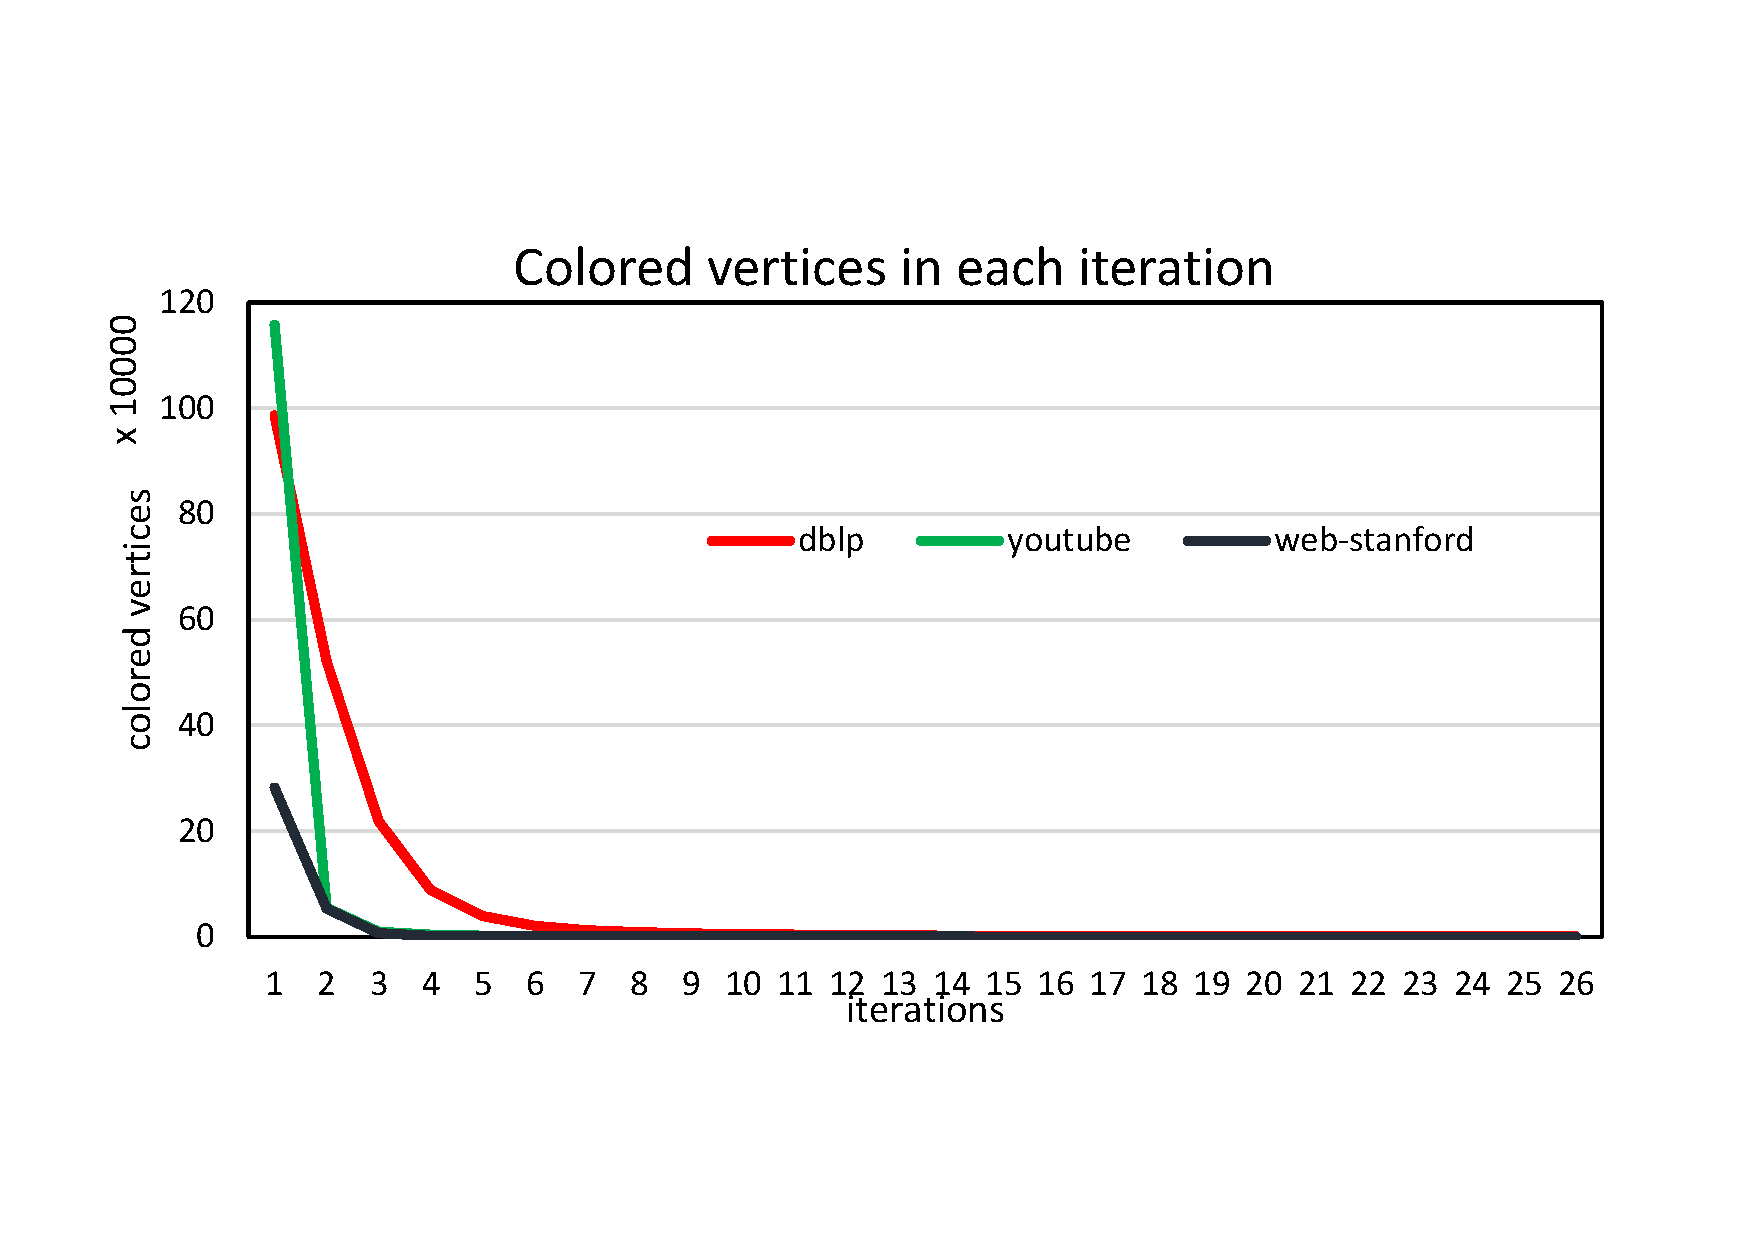
\includegraphics[scale=0.15]{figure/colored_vertices.pdf}
}%
\subfloat[Vertices conflict rate]{
\label{fig:conflict_vertices}
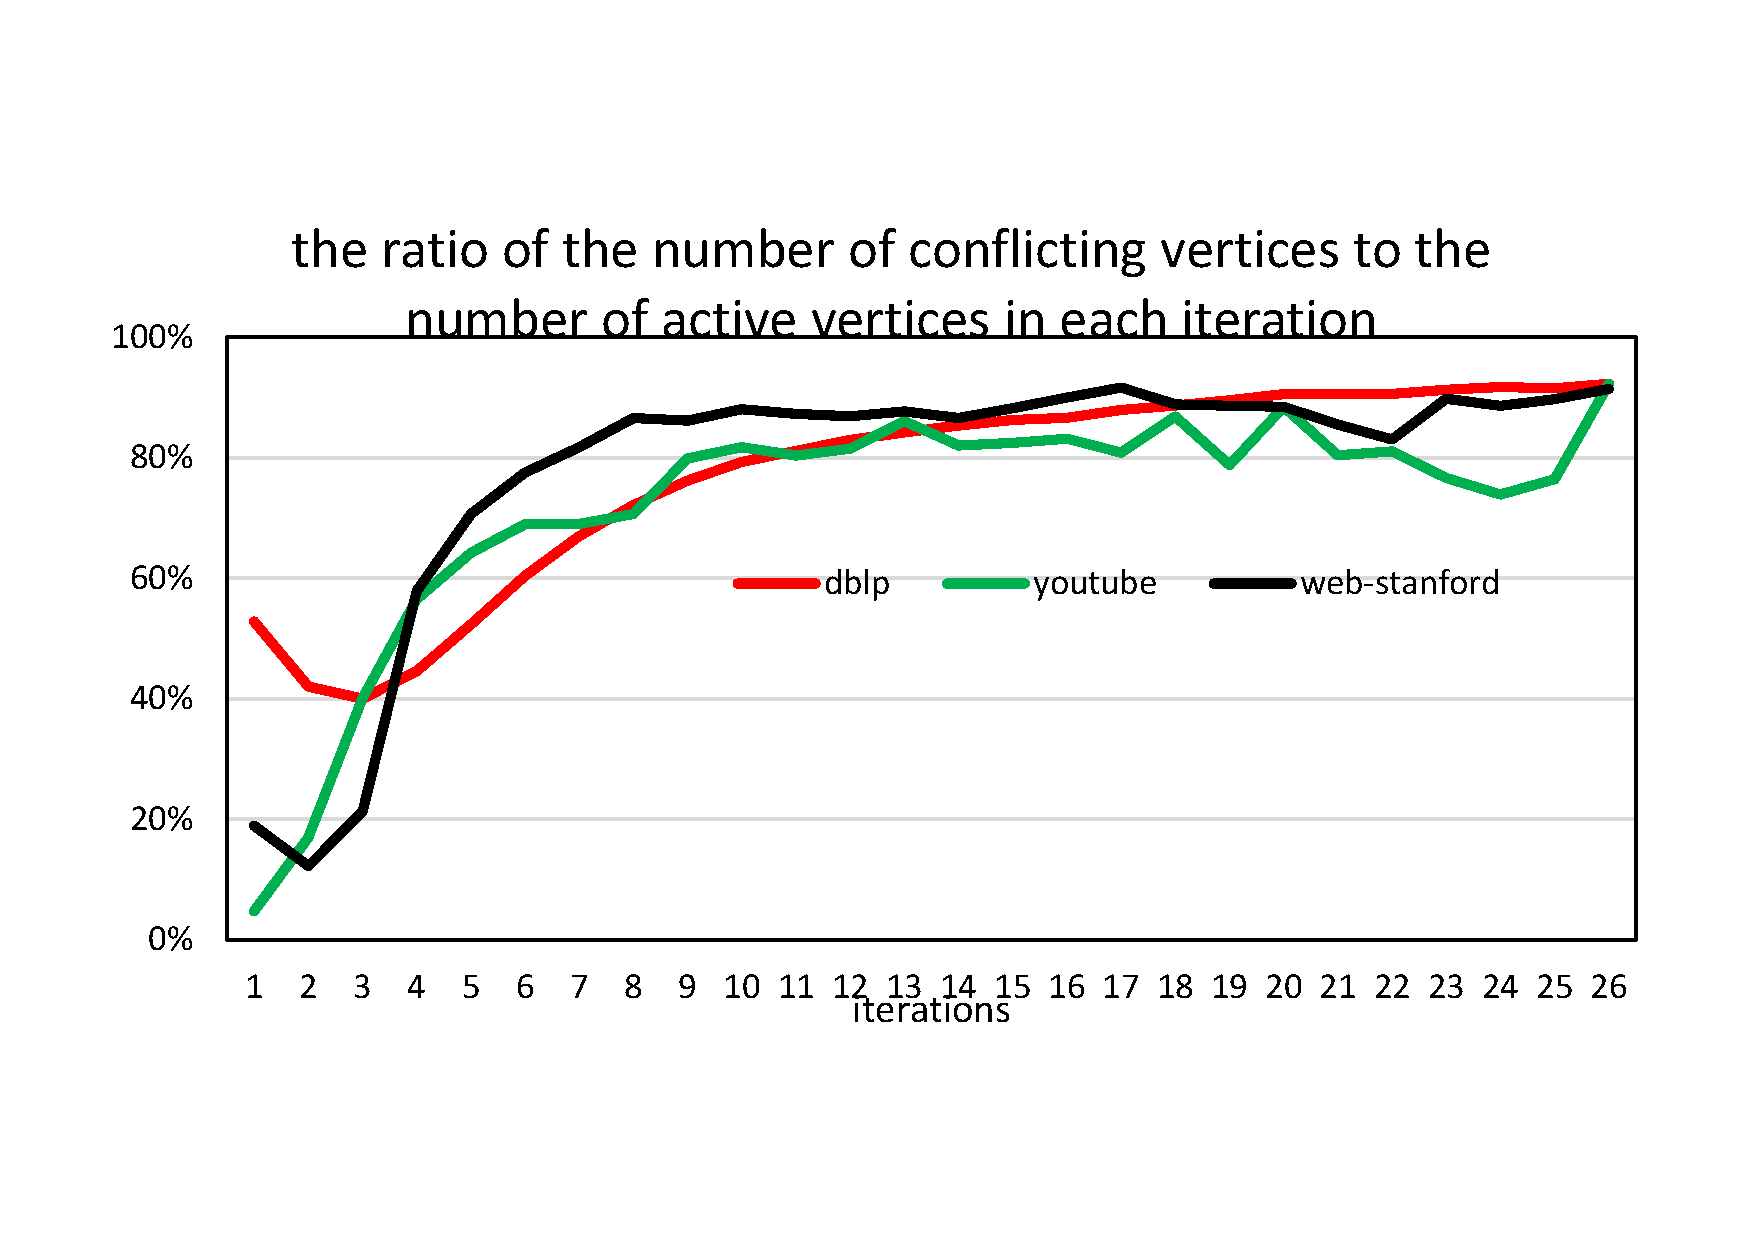
\includegraphics[scale=0.15]{figure/conflict_vertices.pdf}
}%
\caption{The number of colored vertices (Figure \ref{fig:colored_vertices_Iter}) and the ratio of the number of conflicting vertices to the number of active vertices ( figure \ref{fig:conflict_vertices}) as the graph coloring process progress through each iteration. }
\label{fig:colored_vertices}%
\end{figure}

%讲遍历型算法的问题

%In order to demonstrate the problem of sequential spread graph coloring problem, we have conducted the following benchmark experiments. The experiment platform includes a NVIDIA Tesla K20m GPU which equipped with 5 GB on broad memory and 2,496 CUDA cores, and running on Red Hat Enterprise Linux Server release 6.2 (Linux version 3.10.0-514.el7.x86\_64). As we shown in figure \ref{fig:colored_vertices_Tra} the number of colored vertices in each synchronized step is relatively low. From the figure we can conclude that the peak and trough value of the colored vertives are stay in a narrow space except the first few synchronized steps. Which indicates that the active vertices stays almost the same in most synchronized steps.

%讲迭代型算法的问题

Moreover, most recent studies in literature  \cite{Manycore} apply \textit{atomic} operations to implement parallel coloring algorithms on both CPU and GPU. This implementation method greatly restricts the degree of parallelism on GPU. Therefore, it is very useful to develop a graph coloring algorithm that can fully unleash the power of GPU. 

\section{Algorithm Design}
\label{design}

This section presents the design philosophy and describes the algorithm in Feluca.

\subsection{Design Philosophy}
\label{philosophy}

Most of previous coloring research focus on reducing
the number of the colors \cite{vctheory,stoc06,socg14}, which indicates the 
effectiveness of the algorithm. However, improving the coloring efficiency is 
also an important research topic \cite{podc11,jacm11,podc17,podc18}. Most research in this aspect uses either the sequential spread or the recursion-based 
model. However, either of these two models has its own 
limits, as discussed in the motivation section.

In this work, we address the problem in the existing coloring approaches. We present a new
high performance graph coloring algorithm on GPU, the fundamental idea of which is to combine the advantages 
of the recursion and the sequential spread model and avoid their 
drawbacks. 

On the other hand, real-world graphs are growing bigger and bigger, and the graph structure 
is also skewed. another design philosophy of our algorithm is to color as many vertices 
as possible in a round and ensure the scalability of the 
algorithm. 

In summary, there are two targets for our algorithm: i) 
maintaining the coloring effectiveness (with a coloring plan no worse than the existing research) while improving the coloring efficiency (color the graphs faster than current methods), and ii) designing a scalable algorithm, which can easily scale to the system of multi-GPUs for processing large-scale graphs.

In order to meet the above two targets, Feluca has two stages: beginning with the recursion execution model, which can color a majority of vertices in the first few iterations, and then switching to the 
sequential spread execution model once too many conflicts occur. We also propose a novel color-centric coloring paradigm to 
improve the degree of parallelism in the sequential spread stage. 

Further, we develop several GPU-specific optimization techniques including
coalesced memory access and workload balancing, which is presented in Section 4.

All these techniques together comprise an efficient parallel graph coloring 
solution in Feluca. We have conducted extensive experiments on NVIDIA K20m GPU. The results 
show that Feluca can achieve 3.61--125.81$\times$ and 18.58--71.07$\times$ speedup over the greedy coloring algorithm and 
 the existing Jones-Plassman-Luby (JPL) coloring algorithm, respectively. 


\subsection{Two-Stage Graph Coloring Algorithm}
\label{two-stage}

The two-stage graph coloring algorithm is outlined in algorithm %\ref{alg:two-stage}, 
\ref{alg:feluca}. The coloring processing starts on the host. The color array and the graph topology data are then loaded on GPU for coloring. 

\begin{algorithm}[h]
	\caption{Feluca: A High-Performance Graph Coloring Algorithm}
	\label{alg:feluca}
		\begin{algorithmic}[1] %每行显示行号
		\Require Graph, $G$; $fraction$
		\Ensure Graph coloring plan, $COLORS$; and the colors $color\_num$ used for coloring graph $G$;
		\Function {RecursionExec}{$G$}
			\State C(G) $\leftarrow$ init\_color\_randomly(G);
			\While {continue\_flag \&\&  $\frac{colored vertices}{Total vertices} \leq  fraction$}
				\While {$v_j \in V_i$ \&\& $i < j$}
					\If{$c_i == c_j$}
						\State {update $c_j$};
					\EndIf
				\EndWhile
				\If{$continue\_flag$}
					\State ParallelSequentialExec(G);
				\EndIf
			\EndWhile
		\EndFunction
		\Function {ParallelSequentialExec}{$G$}
			\State C(G) $\leftarrow$ init\_color\_randomly(G);
				\While {$continue\_flag$}
					\State traverse\_vertex\_dest(row\_ptr[i], colors);
					\State traverse\_vertex\_src(col\_ptr[i], colors);
					\State row\_ptr[i] $\leftarrow$ colors[i];
					\State col\_ptr[i] $\leftarrow$ colors[j];
				\EndWhile
			\EndFunction
	\end{algorithmic}
\end{algorithm}


In Feluca, we maintain a read-only color array, denoted by \emph{COLORS}, which can be visited by all 
threads. In order to eliminate the conflicts which are caused by the cyclic paths in the graph, we 
change the undirected graph to the directed graph, and set the vertices with lower 
vertex IDs as the source vertices and the vertices with higher vertex ID as destinations.
In our algorithm, we initialize the colors of all the vertices in \emph{COLORS} randomly. 
We define $V_i$ as the set of neighbours of vertex $v_i$ and $c_i$ as the color of $v_i$. 
In the recursion loop, vertex $v_i$ broadcast its own color $c_i$ to its neighbours in $V_i$ following the edges' directions. Once vertex $v_j \in V_i$ receives the color from vertex $v_i$, it compares its color $c_j$ with $c_i$. The comparisons conducted by different vertices are conducted in parallel. If $c_j = c_i$, $v_j$ selects a new color from the \emph{COLORS} array and updates $c_j$. The process repeats until the colors of all vertices in $V_i$ are different 
with the color of $v_i$. 

In the sequential spread stage, %Feluca initialized the graph by using the coloring result of the recursion loop. 
Feluca generates a block of threads and scans the remaining vertices in parallel to find the suitable vertices for each color. In order to improve the degree of parallelism for this algorithm and avoid the conflicts, Feluca assigns a block of threads for each color. The thread blocks for different colors are put into execution in a pipeline. The late blocks can use the coloring results of the early blocks in the pipeline. By doing so, the conflicts in the sequential spread model can also be avoided. 

$N_i$ and $t_i$ denote the colored vertices and the time spent in iteration $i$. $s_i = N_i / {t_i}$ can then be used to express the coloring speed in iteration $i$. The coloring rate (i.e., the percentage of the vertices that have been colored) up to iteration $i$ can be expressed by Equation \ref{eq:lamda}, where $N$ is the total number of vertices in the graph. 

\begin{equation}
\label{eq:lamda}
\lambda = \frac{\sum_{j=1}^{i}{N_j}}{N}
\end{equation}


Feluca switches to the sequential spread coloring method once the color rate ($\lambda$) in the recursion stage is lower than the value of the parameter $fraction$. $T$ denotes the total coloring time. We can have $T=\sum_{i=1}^{r}{t_i}+\sum_{j=r+1}^{r+s}{t_j}$, where $r$ is the number of iterations in the recursion stage while $s$ is the number of iterations in the sequential spread stage. 
%$V_R$ and $V_S$ denote the number of colored vertices in the recursion stage and the sequential spread stage, respectively. 
%We have $V_R= \sum_{i=1}^{r}{N_i} =\lambda N $, and $ V_S = \sum_{j=1}^{s}{N_j}=(1-\lambda)N$. Hence, $T = \lambda f(s_r) t_r + (1- \lambda) f(s_s) t_s$, which is a convex optimization problem and there exist an appropriate $\lambda = fraction$ to make $T$ get its minimum value, we will show how can we choose a suitable $fraction$ in section \ref{experiments}, where $f(s_r)$, $f(s_s)$ and $t_r$, $t_s$ are the coloring speed and average coloring time for each iteration of recursion and sequential spread stage respectively.
Hence, we can express the coloring time as formula \ref{eq1}.

\begin{equation}
\label{eq1}
		T=\sum_{i=1}^{r}{t_i}+\sum_{j=r+1}^{r+s}{t_j}=\sum_{i=1}^{r}\frac{N_i}{s_i}+\sum_{j=r+1}^{r+s}\frac{N_j}{s_j}
\end{equation}

Furthermore, we use $s_{rmin}$, $s_{rmax}$ and $s_{smin}$, $s_{smax}$ to denote the minimum and maximum value of the coloring speed at recursion and sequential spread stage, respectively. Then we can express $T$ as formula \ref{eqt}.

\begin{equation}
\label{eqt}
		\sum_{i=1}^{r}\frac{N_i}{s_{rmax}}+\sum_{j=r+1}^{r+s}\frac{N_j}{s_{smax}} \leq T \leq \sum_{i=1}^{r}\frac{N_i}{s_{rmin}}+\sum_{j=r+1}^{r+s}\frac{N_j}{s_{smin}}
\end{equation}


Combining equation \ref{eq:lamda} and  formula \ref{eqt}, we can have formula \ref{eqtt}.

\begin{equation}
\label{eqtt}
		\frac{\lambda \times N}{s_{rmax}}+\frac{(1-\lambda) \times N}{s_{smax}} \leq T \leq \frac{\lambda \times N}{s_{rmin}}+\frac{(1-\lambda) \times N}{s_{smin}}
\end{equation}

Formula \ref{eqtt} indicates that $T$ can be formulated as the form of function over $\lambda$ shown in formula \ref{eq2}, where $s_r$ and $s_s$ are the coloring speed in the recursion stage and sequential spread stage, and $t_r$ $t_s$ are the coloring time spent in the recursion stage and sequential spread stage, respectively, and $f_1(t_r)$ and $f_2(s_s)$ are the functions that takes $s_r$ (or $t_r$) and $t_s$ as input, respectively. 

\begin{equation}
\label{eq2}
		T= \lambda f_1(s_r) + (1-\lambda)f_2(s_s) = \lambda f_1(\frac{N}{t_r}) + (1-\lambda)f_2(\frac{N}{t_s})
\end{equation}

It can be seen from equation \ref{eq2} that finding a minimum $T$ is a convex optimization problem. We will show how we choose a suitable value $fraction$ for $\lambda$ in section \ref{experiments}. When the color rate $\lambda$ is higher than $fraction$, the graph coloring in Feluca switches from the first stage (recursion) to the second stage (sequential spread). 
\section{Optimization Techniques on GPU}
\label{optimization}

In this section, we presents the optimization techniques on GPU to improve the algorithm efficiency.

\subsection{Eliminating Cyclic Paths and Atomic Operations}
\label{eliminate}
When the recursion-based coloring algorithm works on cyclic graphs, it is easy to fall into an infinite loop since 
the algorithm runs following the edge's direction. In order to solve this problem, we develop a method in Feluca to eliminate the cyclic paths in the directed graphs. In the method, Feluca checks all the vertices $v_j \in V_i$ (i.e., the set of neighbours of vertex $v_i$) before coloring $v_i$, and changes the edge $<v_i, v_j>$ to $<v_j, v_i>$, if $i>j$. For example, the edge $<v_4, v_1>$ in figure \ref{fig:color_a} is changed to $<v_1, v_4>$ in figure \ref{fig:color_b}. The change of edge direction does not affect the coloring plan. For example, these two coloring scheme in figure \ref{fig:color_a} and figure \ref{fig:color_b} are regarded as same.  

\begin{figure}[h]
\centering
\subfloat[Cyclical graph coloring]{%
\label{fig:color_a}
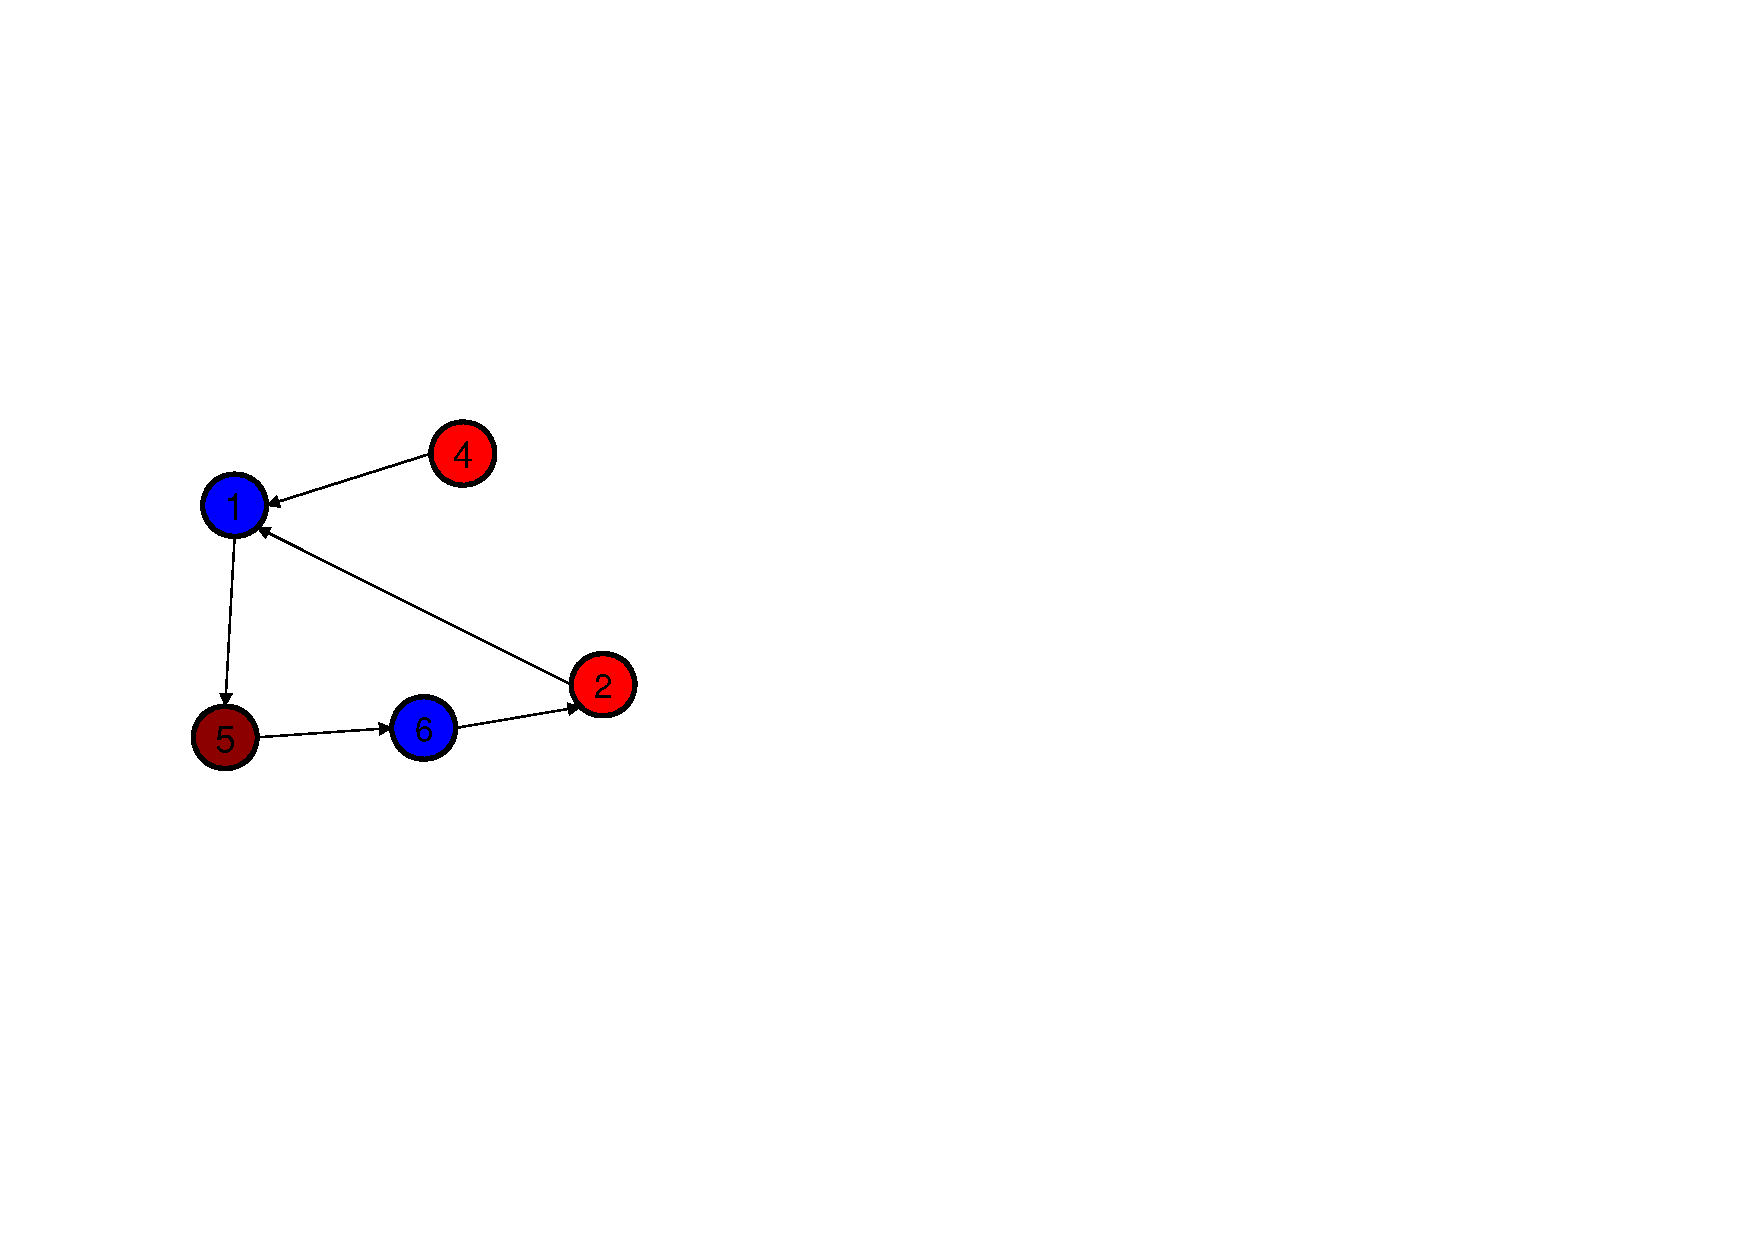
\includegraphics[scale=0.4]{figure/color_b.pdf}
}%
\hspace{0.4in}
\subfloat[Acyclic graph coloring]{
\label{fig:color_b}
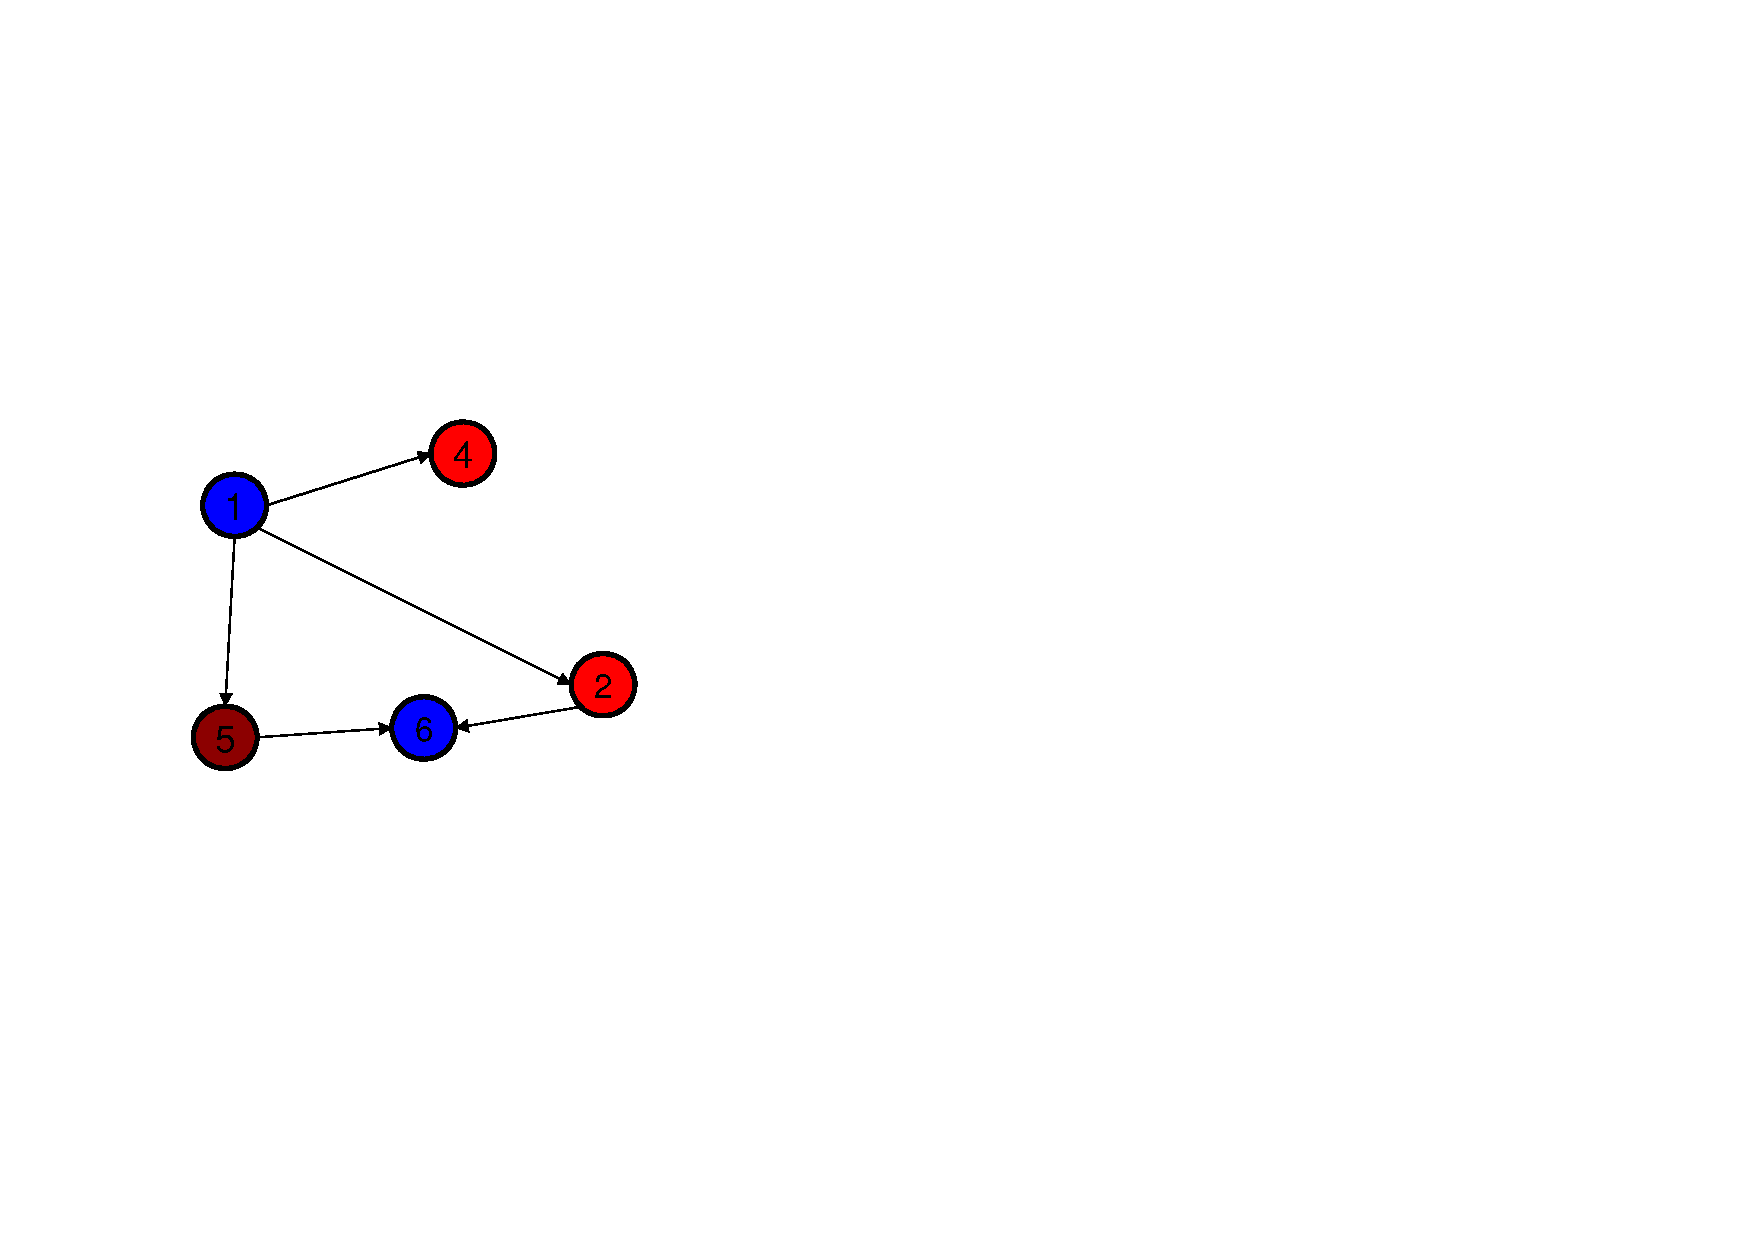
\includegraphics[scale=0.4]{figure/color_a.pdf}
}%
\caption{Coloring scheme for cyclical graph and acyclic graph.}
\label{fig:color_scheme}%
\end{figure}

Dynamic conflict list, which is an array used to store the vertices (or edges) to be processed in the subsequent iterations/loops, is widely used in both vertex-based and edge-based graph processing models. In graph coloring, the dynamic conflict list is used not only 
to maintain the upcoming workload, but also to store the candidate colors in the color array. 
A typical coloring algorithm traverses the color array to select a suitable color 
for current vertex. Because of the SIMD execution model in GPU, a massive number of threads access the 
color array simultaneously. The \emph{atomic} operation is widely 
used to manage the simultaneous accesses to a common array on GPU. Atomic operations suffer from the heavy overhead when there are frequent accesses. Moreover, atomic operations might result in a scattered conflict list,  
where the consecutive vertices are store far apart in locations.

Eliminating atomic operations on GPUs for maintaining 
the coloring array have been considered in previous work 
\cite{vldbcolor,Manycore}. Reference \cite{Manycore} 
is a representative graph coloring work on many-core architectures 
(including Xeon Phi and GPU). In their work, the authors defined two 
arrays. One is used to hold the forbidden colors for the active 
vertex $v$ while the other is used to select the smallest available 
colors. The two arrays are named \emph{VFORBIDDEN} and \emph{ASSIGNCOLORS}, respectively. 
The authors use atomic operations to maintain these two arrays. 
This approach is inefficient, because it cannot avoid the atomic 
operations fully and more memory space is needed for \emph{VFORBIDDEN} than 
traditional traversal algorithms. Figure \ref{fig:atomic} shows 
an example of typical color array on GPU with atomic operation. 
As we shown in figure \ref{fig:atomic}, when the algorithm colors 
vertex 1 and 5, the two threads that are processing these two vertices 
need to visit the color array simultaneously. To ensure that
both threads can get the right color, the atomic operation is needed. 

\begin{figure}[h]
\centering
\subfloat[Sample graph]{%
\label{fig:sample-graph}
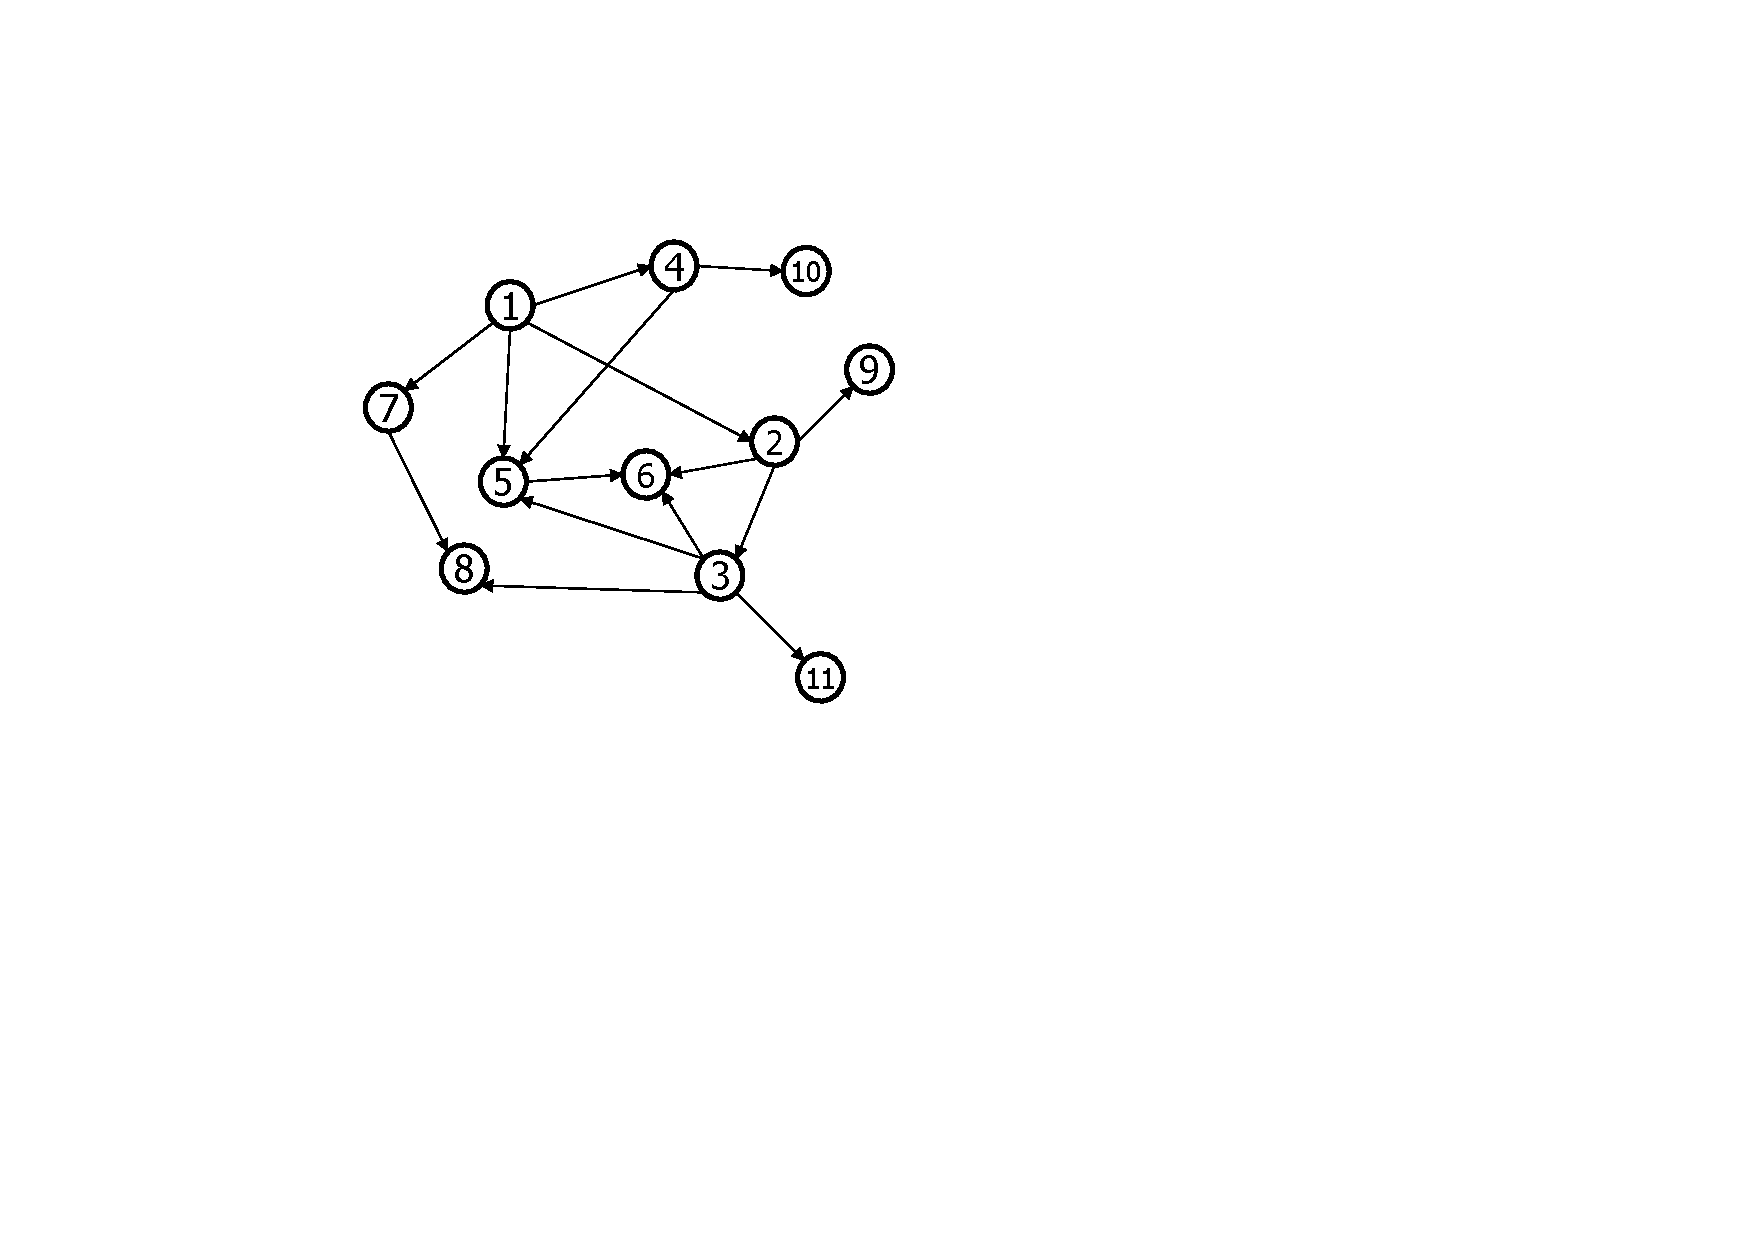
\includegraphics[scale=0.35]{figure/samplegraph_re.pdf}
}%
\subfloat[Color selecting]{
\label{fig:out-degree}
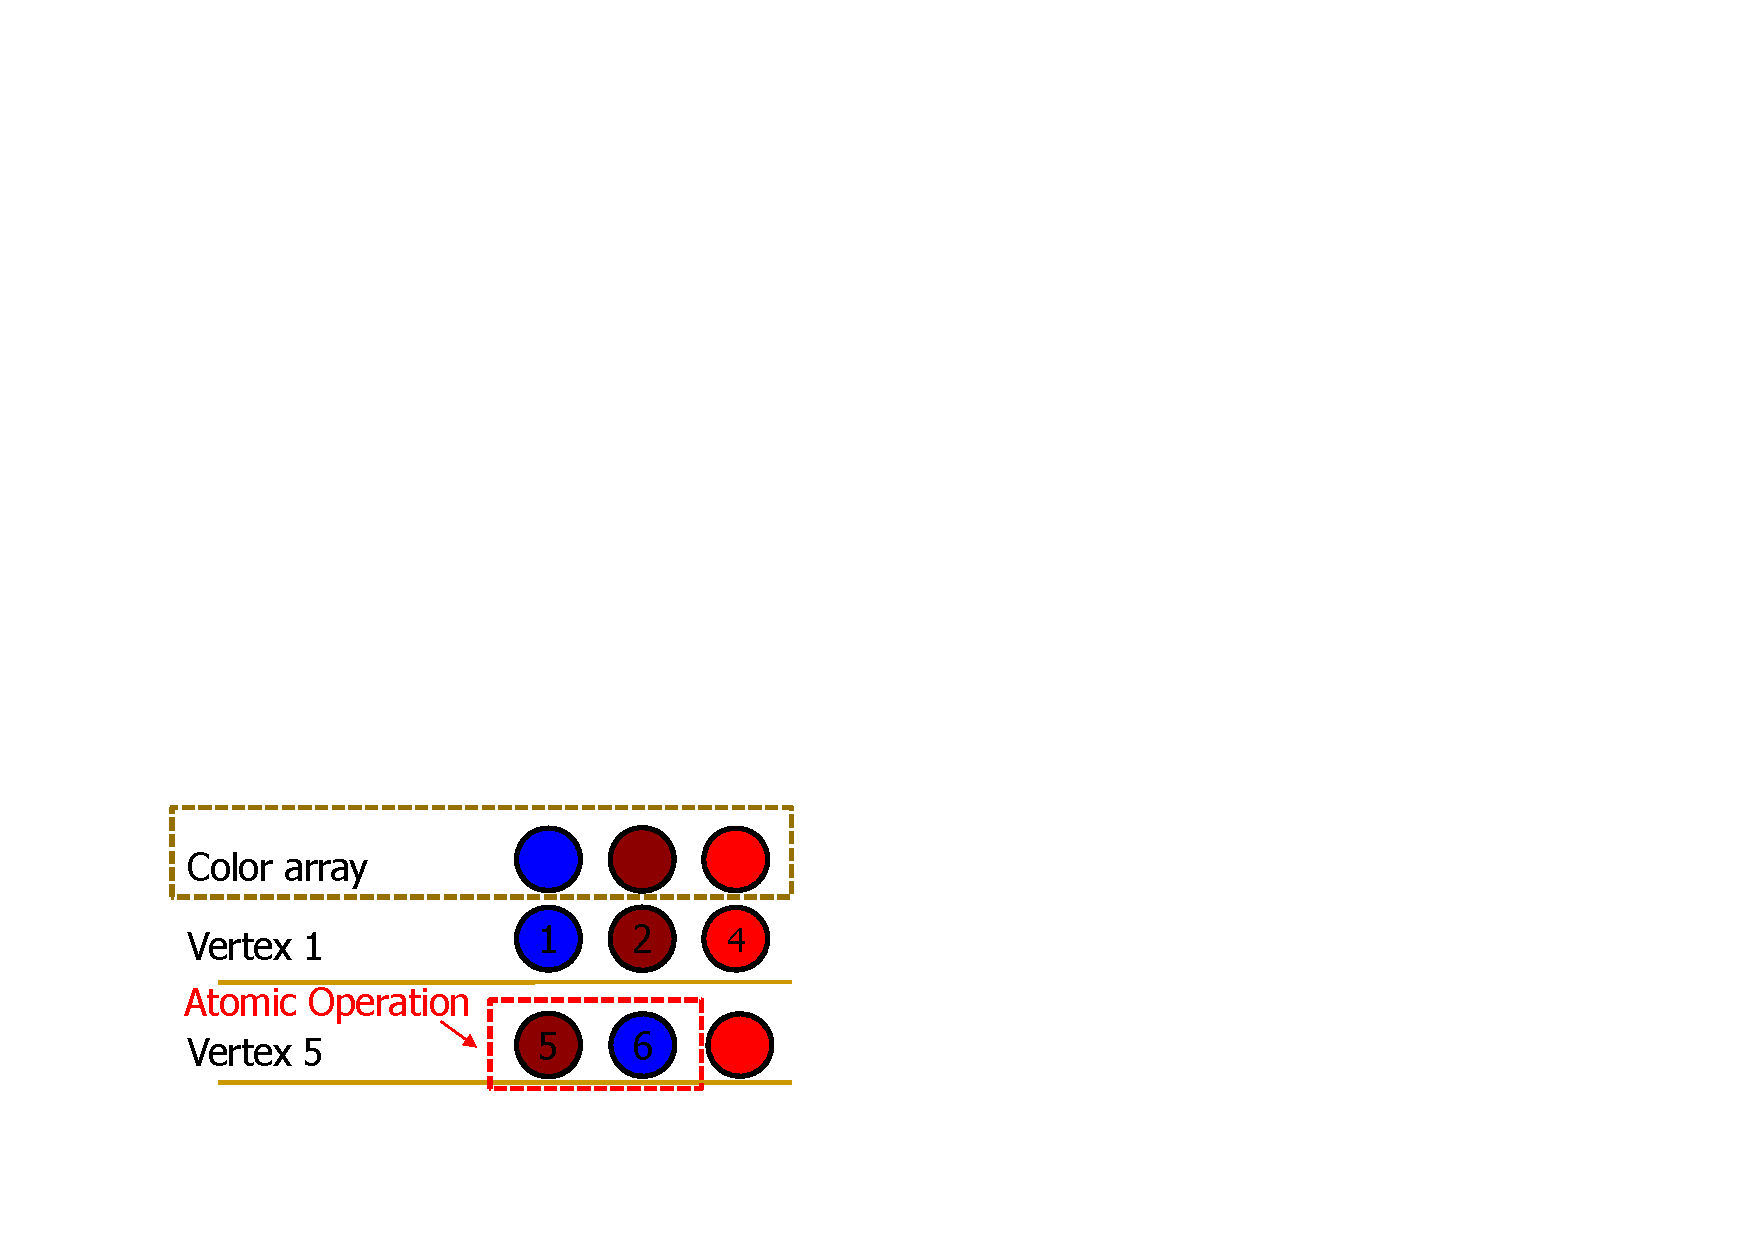
\includegraphics[scale=0.45]{figure/color-selecting.pdf}
}%
\caption{An example of typical color array with atomic operation.}
\label{fig:atomic}%
\end{figure}
 
There are several ways to resolve the color conflicting, such as selecting another new color randomly or assigning first available color when conflicts occur.  
But these methods may lead to a huge color set in the final result. Choosing the first available color is the most widely used method. In this method, 
the algorithm searches along the color array to find the first available color (i.e., the color is 
not used for previous vertices). As a massive number of threads are running in parallel for 
a GPU kernel, the atomic operation or lock is needed to ensure that every thread can 
find the right color. This will slow down the coloring process greatly. In Feluca, 
a top-down color selection scheme is 
proposed to select the suitable color for the conflicting vertices. This scheme can avoid the atomic operations fully. We detail the working of our color selection scheme next. 

As presented earlier in this section, we have transformed the graph to a directed acyclic graph (DAG). Our top-down coloring scheme starts coloring from the top level  (root) of the graph, and traverses the graph in the same way as the BFS (Bread-First-Search) algorithm. There are often multiple vertices in a graph level, which are colored by multiple threads in parallel. After a level of vertices are colored, the coloring scheme moves onto the next level in the DAG graph (hence a top-down coloring scheme), and the computation moves into next iteration. The process repeats until all vertices have been colored. 

A color array is used to hold all used colors. When a new color has to be used for a vertex, the new color is appended at the end of the color array. 

After a thread has colored a vertex in a level, it finds the neighbours of this vertex following its outgoing edge. The neighbours are the vertices in the next level, which are also the vertices ready to be colored in next iteration. When a thread is trying to color a vertex in an iteration (suppose in iteration $i$), it checks the colors assigned to this vertex's parents in last iteration (iteration $i-1$) and then assigns to this vertex the color that is immediately after the last color among all parents' colors in the color array. 

An example is illustrated in figure \ref{fig:colorsec} to show how our top-down coloring scheme works. The exemplar graph is still the one in figure 3. In figure \ref{fig:colorsec}, suppose the graph coloring is currently in iteration $i$. It can be seen from figure 3 that vertices 1 and 4 are the parents of vertex 5. Therefore when the coloring scheme colored vertices 1 and 4 in iteration $i-1$ (assume the colors assigned to vertices 1 and 4 are blue and red, respectively as shown in figure \ref{fig:colorsec}), it followed the edges $<1, 5>$ and $<4, 5>$ to find that vertex 5 is a vertex to be colored in iteration $i$. Now suppose the coloring scheme is trying to color  vertex 5 in iteration $i$. Our coloring scheme realizes that vertices 1 and 4 are the parents of 5. Then, it assign the color that is immediately after the colors of vertices 1 and 4 (blue and red), which is cyan, to vertex 5. The traditional coloring scheme would search the whole color array to find the first available color, which would assign ``dark red" to vertex 5 in this example. Our coloring scheme only needs to check the colors of the parents assigned in last iteration and does not need to search the entire color array. 

Our color chosen scheme only focuses on the current vertex and its parent vertices colored in last iteration. This design enables the GPU threads to update the colors of their current vertices in parallel without atomic operation/lock. 

\begin{figure}[h]
	\centering
		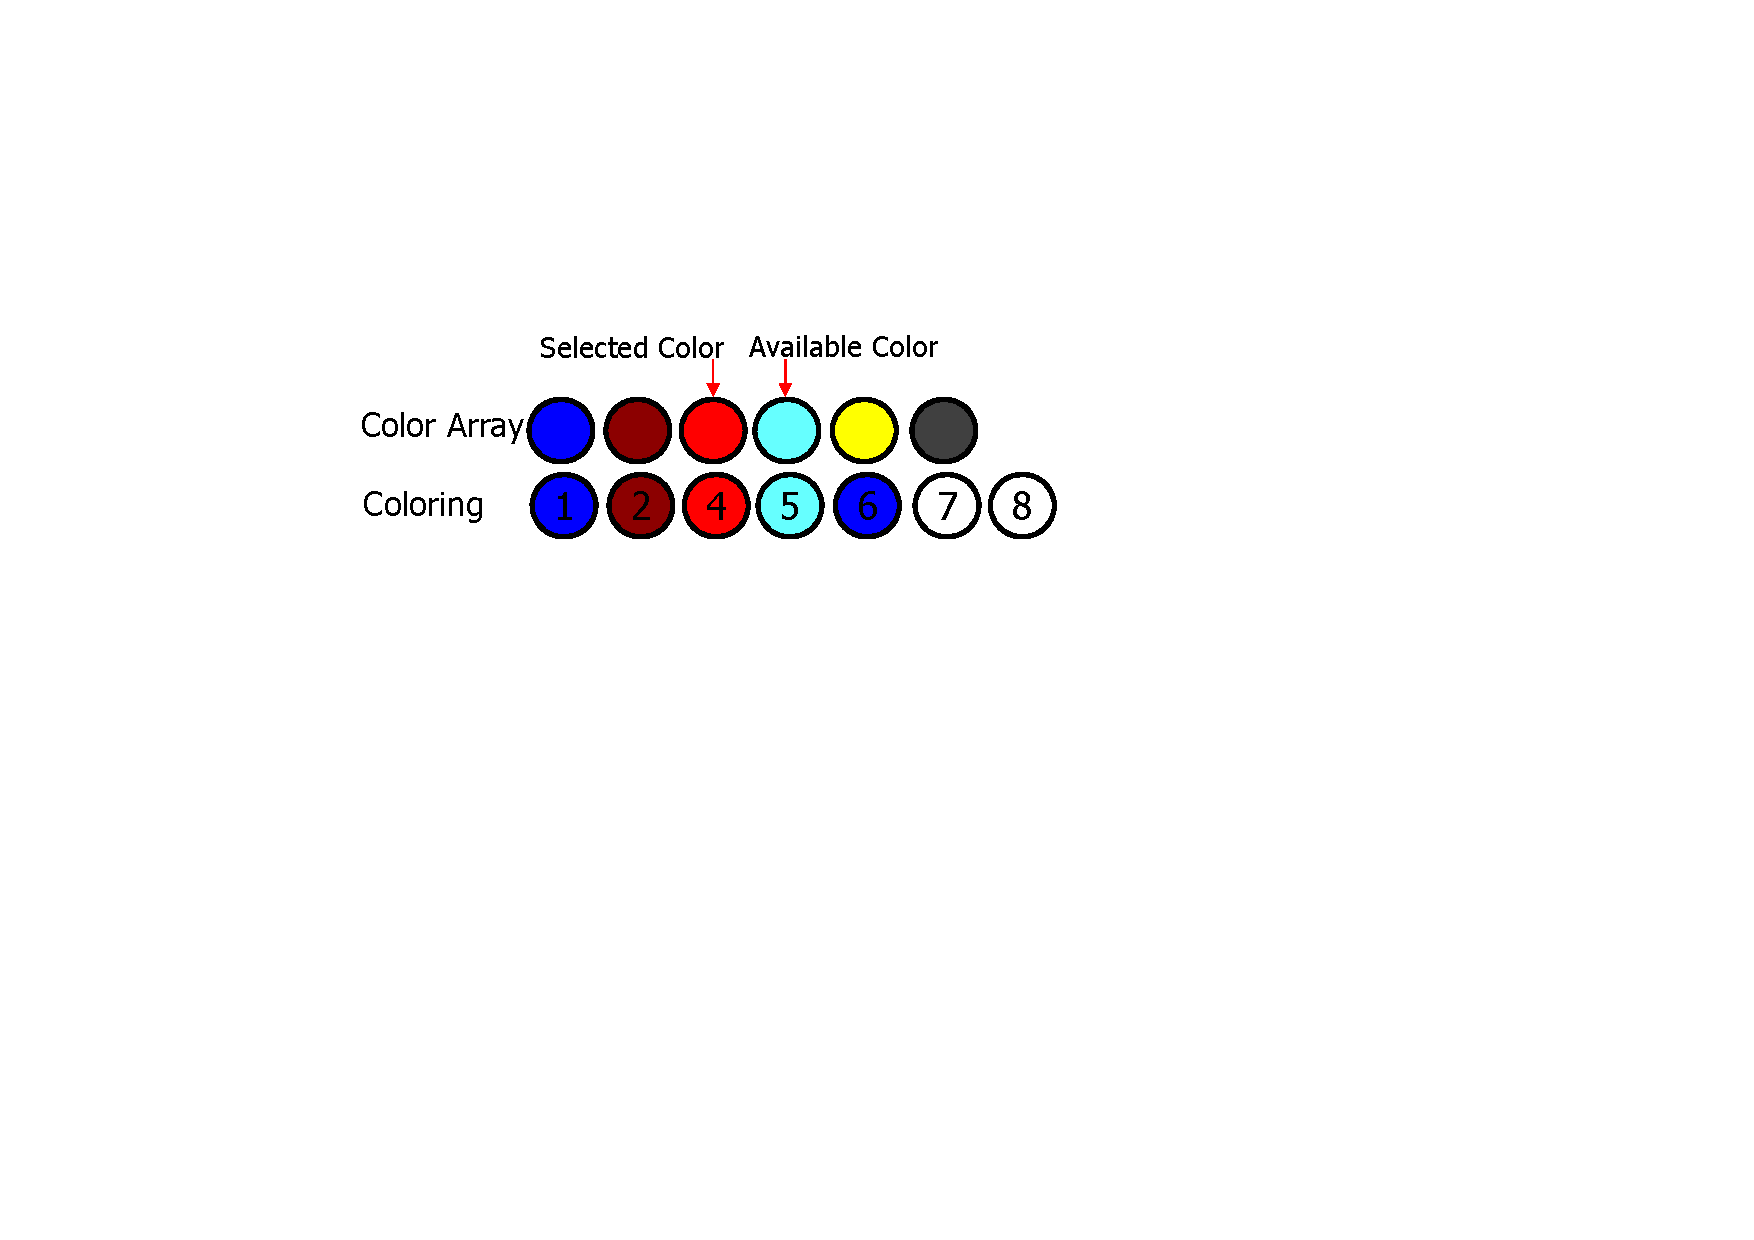
\includegraphics[scale=0.4]{figure/colorsec_re.pdf}
	\caption{The top-down coloring scheme in Feluca. The ``Selected color'' is the last color assigned to the parents of vertex 5 in iteration $i-1$. Then the color labelled as ``Available Color" will be assigned to vertex 5 in iteration $i$.}
	\label{fig:colorsec}%
\end{figure}

\subsection{Color-centric Coloring Paradigm}
\label{color-centric}

When GPU is used to accelerate graph processing, threads in GPU are organized in a grid and all the threads in a grid execute the same kernel function. The threads running a kernel are organized in a two-level hierarchy: a grid consists of a number of thread blocks and each block comprises a set of threads. It is a great challenge to parallelize the sequential spread coloring, because coloring the vertices in iteration $i$ depends on the results of iteration $(i-1)$.
In order to improve the degree of parallelism of the sequential spread stage in Feluca, we proposed a new coloring scheme, called the color-centric scheme. 
The traditional algorithm for sequential spread coloring is vertex-centric, i.e., finding a suitable color for each vertex. In our color-centric scheme, we find all suitable vertices for each color, which is presented in detail next. 

After the first coloring stage (the recursion stage) is finished, we record all the remaining vertices which have not converged to the final colors yet (called uncolored vertices).  
In the color-centric scheme, for each color, we generate a thread block to find in the list of remaining un-colored vertices all vertices that can be assigned with this color. A thread block starts with the uncolored vertices in the first graph level, and moves down the graph levels until all uncolored vertices have been colored. 

In the color-centric scheme, different thread blocks find vertices for different colors in parallel. We develop two parallelization strategies to run the thread blocks for each color. In the first parallelization strategy, we set the number of colors needed for the remaining uncolored vertices. We then generate a thread block to find all vertices for each color. In particular, a thread block for a color collectively find all vertices that do not have direct links between any two of them and assign all these vertices to this color. We start the execution of all thread blocks at the same time. In this strategy, it is possible that different thread blocks assign different colors to the same vertex. When this happens, the vertex keeps the color which has the smallest color ID among the conflicting colors. The shortcoming of this parallelization strategy is that we have to first set the number of colors for the remaining uncolored vertices. We cannot accurately know the exact number of colors needed. On one hand, if the number of colors is set too low, it is impossible to deliver the final coloring plan which does not contain conflicting. On the other hand, if the number is set too high, the number of colors in the final coloring plan will be much higher than that in the optimal coloring plan. 

In the second parallelization strategy, we do not start all thread blocks at the same time, but run the thread blocks in pipeline. In particular, we first start the thread block for the first color. The thread block starts with find all uncolored vertices in the first level of the graph that can be assigned to the first color. After the first level is processed, the thread block moves to the second level and repeats the process. While the thread block for the first color is processing the second level, we start the thread block for the second color and start to find all remaining uncolored vertices that can be assigned to the second color. Similarly, when the thread block for the first color moves to the third level, the thread block for the second color moves to the second level and the thread block for the third color start processing the first level. The pipeline goes on until all uncolored vertices after the recursion stage have been colored. In the second strategy, we do not have the problem that we may set the number of colors too high. When all vertices have been colored, the pipeline stops and the number of used colors then is the number of colors in the final coloring plan. Our experiments show that the first and second parallelization strategies have similar running performance. But the second strategy typically uses a fewer number of colors than the first strategy. Therefore, we use the second parallelization strategy in the sequential spread stage in Feluca. 

\subsection{The Edgelist Graph Representation}
\label{edgelist}
A GPU can reach its peak memory 
access bandwidth only when the algorithm has a regular memory access pattern, 
i.e., the data accessed by the consecutive threads of a warp occupies the 
contiguous memory locations. 
When there is no a regular memory access pattern, a naive solution to improve the GPU memory access efficiency is to sort 
the edges by source vertex ID, which is shown in figure \ref{fig:edgelistrep}. 
Figure \ref{fig:edgelistrep} shows the edgelist representation of the graph in figure \ref{fig:sample-graph}. 
The graph has 11 vertices and 15 edges. The 15 edges are partitioned into 4 edge blocks. In this partition, the edges are 
sorted in the order of their source vertex IDs and every edge block contains 4 edges. Suppose that 
a warp contains 4 threads. Then a warp can process the whole block.
But in this partition, the edges with source vertex ID 3 are allocated to 2 
blocks. Hence, the threads processing the edges with source vertex 2 in 
block 2 need to wait for the threads which process the edges with source 
vertex ID 3. It is also the case for the threads which process 
with source vertex 4. When processing the real-world graphs, the edges of 
high degree vertices may be scattered in several blocks. On the other hand, a block 
may contain the edges from more than one low-degree vertex. Under this circumstance the computing load of different edge blocks vary, which will cause 
the threads in a thread block to wait for other thread blocks with more computing load. 

\begin{figure}[h]
\centering
\subfloat[The edgelist representation of the graph in figure \ref{fig:sample-graph}.]{%
\label{fig:edgelistrep}
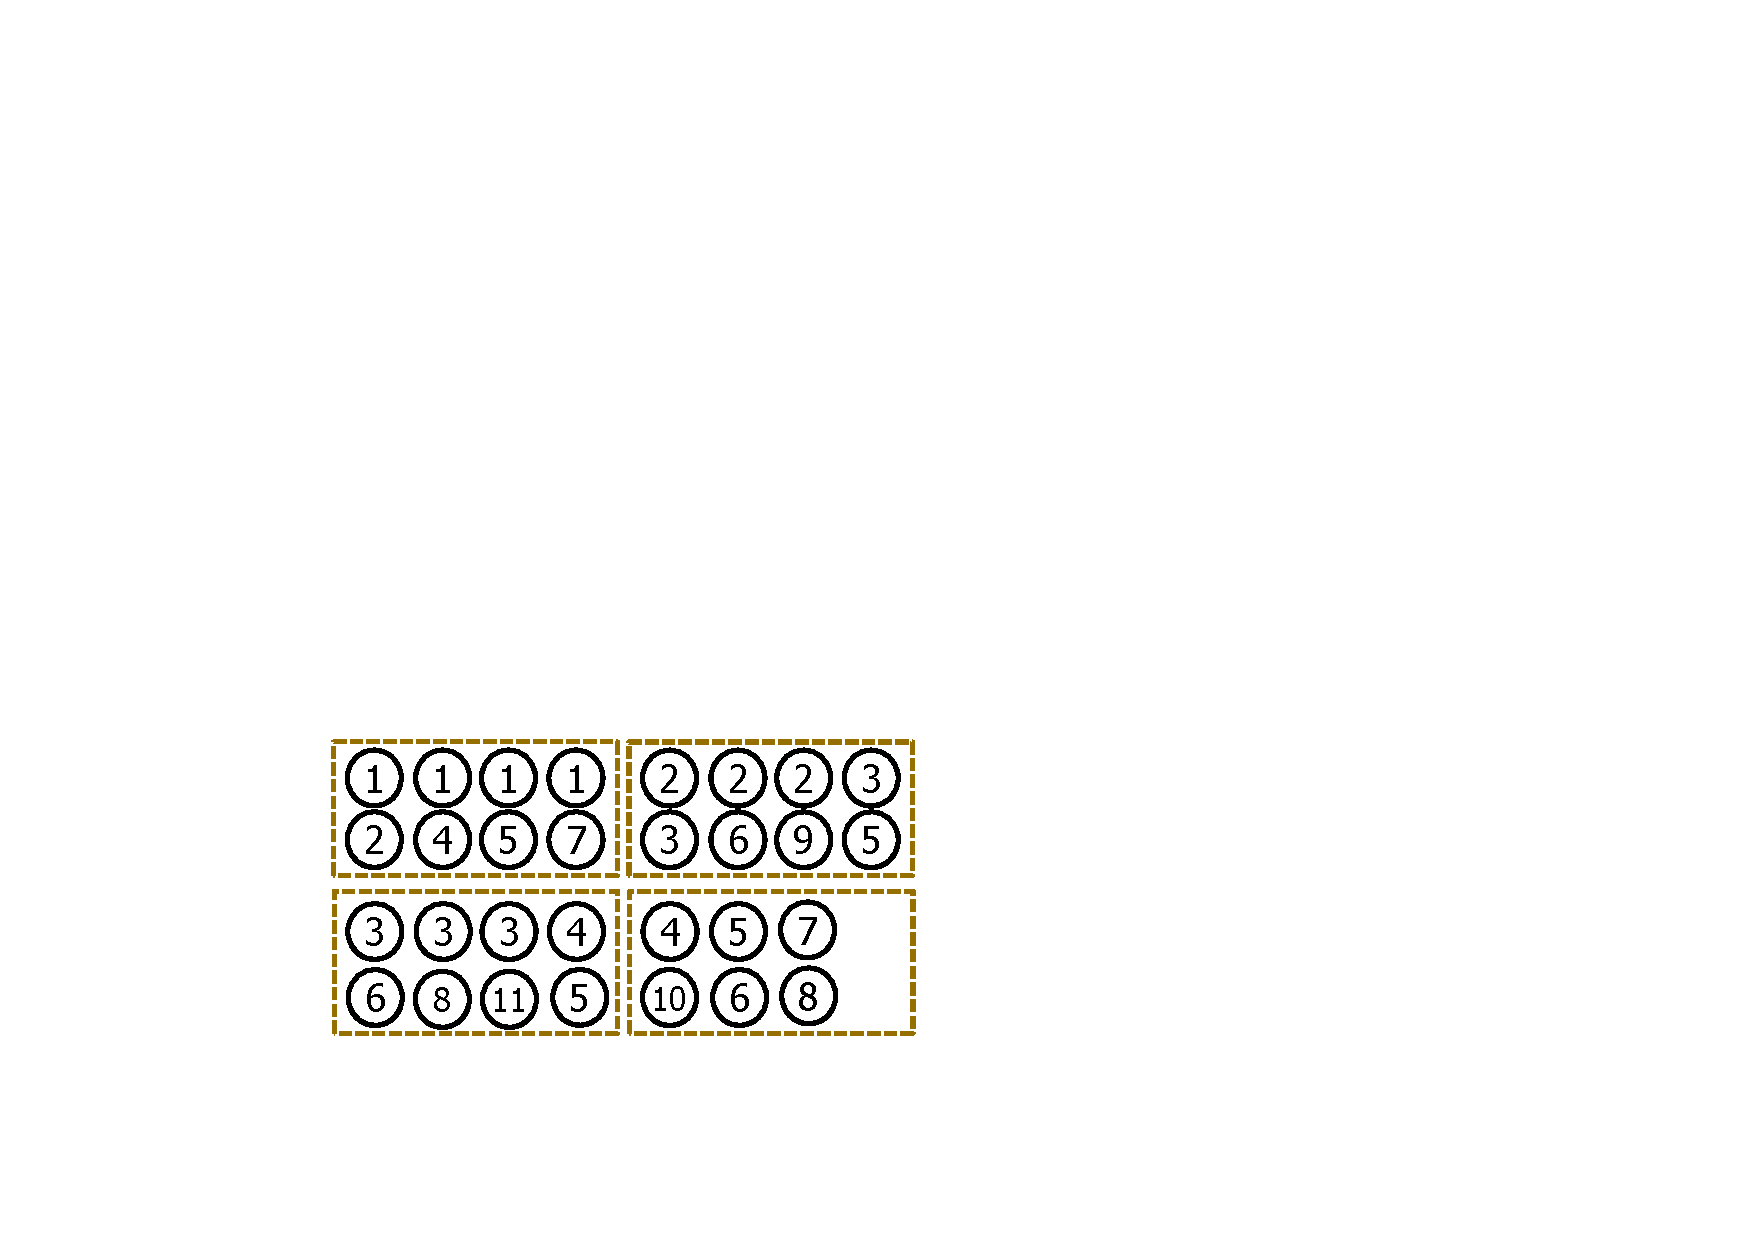
\includegraphics[scale=0.4]{figure/edgelist_re.pdf}
}%
\subfloat[The ordered graph with virtual edges.]{
\label{fig:rep}
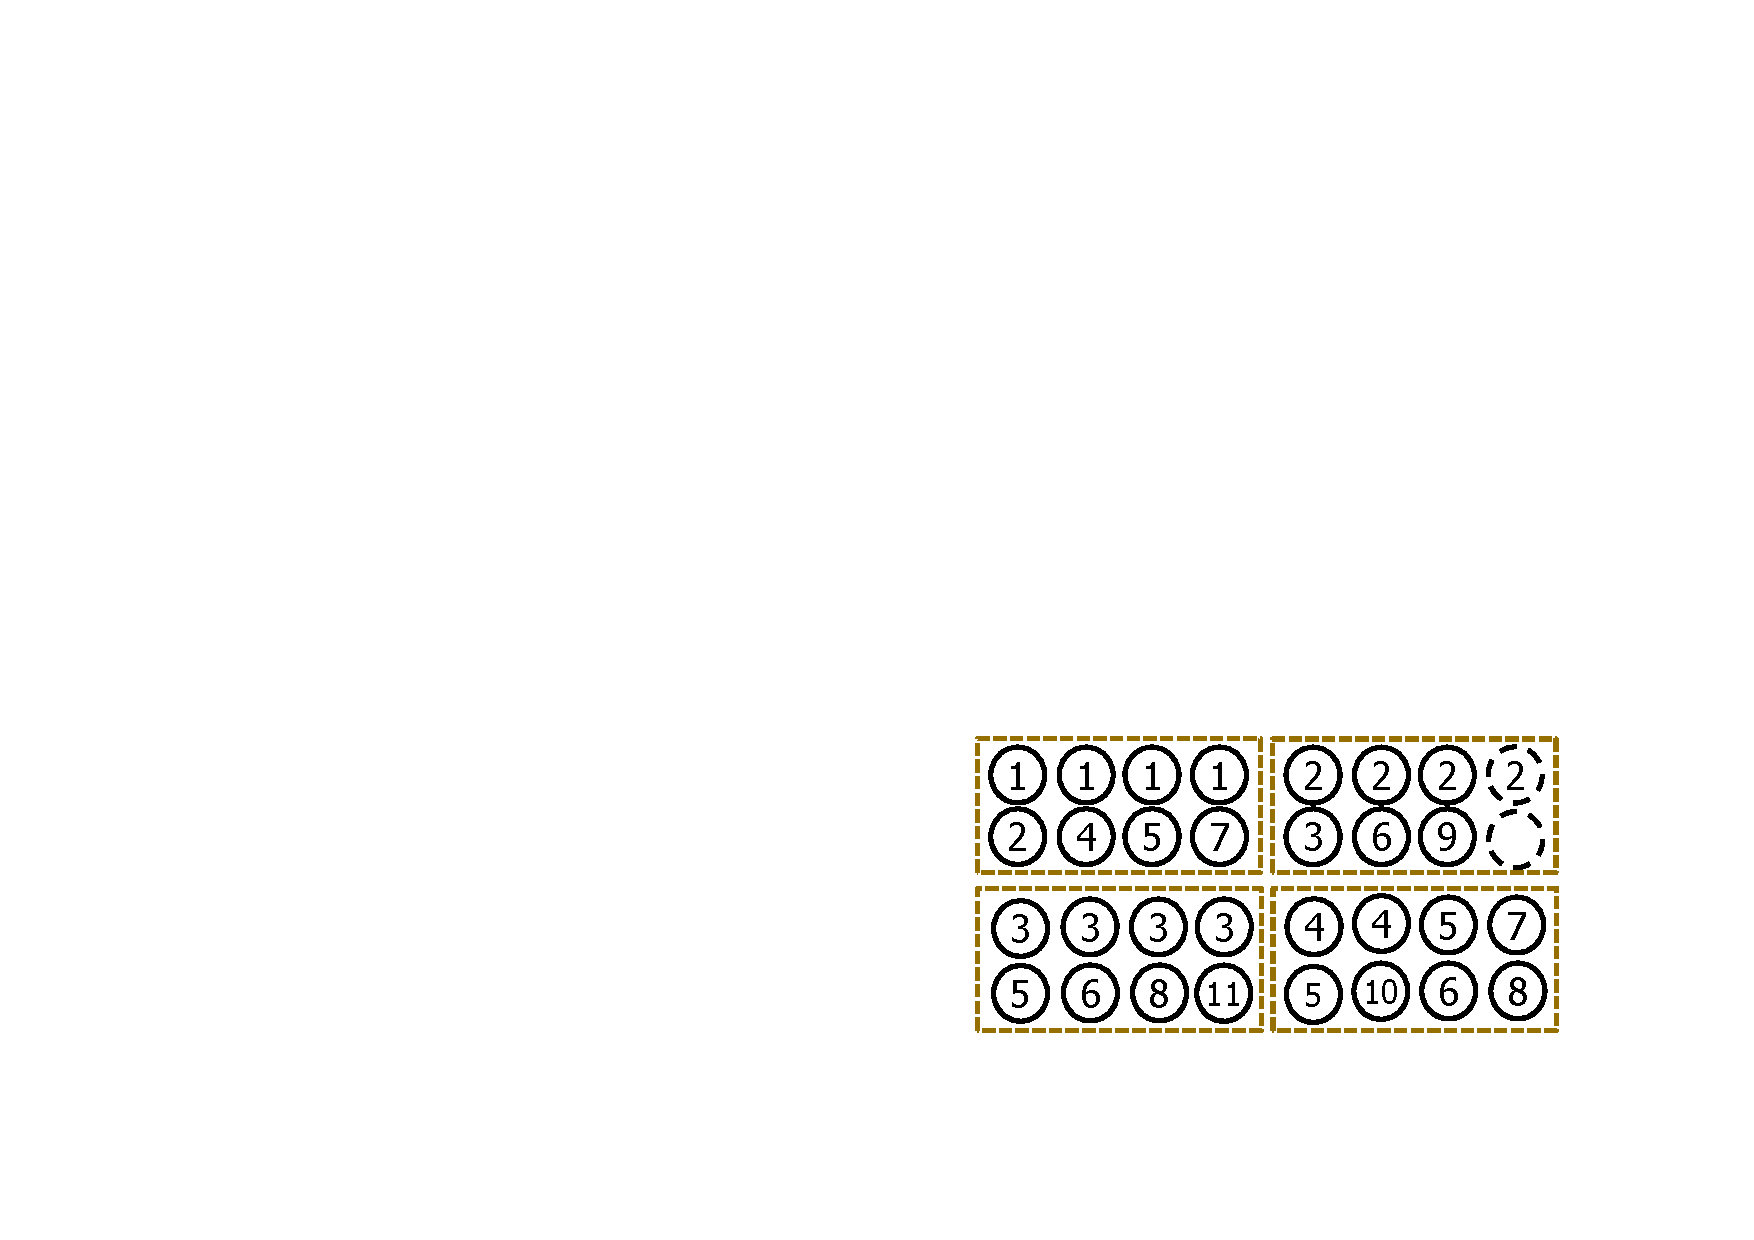
\includegraphics[scale=0.4]{figure/rep_re.pdf}
}%
\caption{An example of ordering the graphs by adding virtual edges.}
\label{fig:virtual_edges}%
\end{figure}

In order to address this problem, Feluca adds some virtual edges, which do 
not take any memory space, in the edgelist-based graph representation such that either the edges in an edge block have the same source ID or an edge block contains all edges from different vertices. 

For example, We add a virtual edge with source vertex ID 2 as shown in figure \ref{fig:rep}. In the ordered graph, all the 
edges with source vertex ID 1, 2 and 3 are located in a single warp and all the 
remaining edges are located in the same warp (i.e., the warp contains all edges for vertice 4, 5 and 7). This representation can avoid the 
overhead that the threads wait between the edges with source vertex 2 and 3. As edges 
are sorted in the order of the source vertex ID in the grid, continuous and coalesced memory 
access pattern can be achieved.
\section{Evaluation}
\label{experiments}

In this section, we present the results of experimental evaluation for different design choices in Feluca and compare Feluca with the state-of-the-art graph coloring techniques on both power-law and random graphs.

\subsection{Experimental Setup}
\subsubsection{Data Format}
\label{subsec.format}
We have conducted the experiments with both directed and undirected graphs. $(u, v)$ represents the undirected edge between vertices $u$ and $v$ while $<u, v>$ represents a directed edge from $u$ to $v$.

A graph is stored in a plain text file, in which each vertex has an unique ID and there are a list of directed or undirected edges, one edge per line. As mentioned in Section~\ref{design}, an undirected graph is converted into the directed graph by setting an edge's direction from the vertex with a lower ID to the vertex with a higher ID. Considering only the single direction of an undirected edge is sufficient to solve the color conflicts.

\begin{table}[h]
\centering
\caption{Datasets used in the experiments}
\label{tab:datasets}
\begin{tabular}{|l|r|r|r|}
\hline
 Datasets					&Vertices						&Edges					&Direction\\\hline
 web-Stanford			&281,903						&2,312,497			&Directed \\
% Amazon						&735,322						&5,158,012			&Undirected \\
 dblp							&986,207						&6,707,236			&Undirected \\
 youtube					&1,157,828					&2,987,624			&Undirected \\
 RoadNet-CA				&1,971,282					&5,533,214			&Undirected \\
 Wiki-Talk				&2,394,385					&5,021,410			&Undirected \\
% com-orkut				&3,072,626					&117,185,083		&Undirected \\
 soc-LiveJournal	&4,847,571					&68,993,773			&Directed \\
 RMAT16-2					&9,999,993					&160,000,000		&Undirected \\
 random-graph			&19,999,888					&100,000,000		&Undirected \\
 twitter-2010			&41,652,230					&1,468,365,182	&Directed \\
 webbase-2001			&118,142,155				&1,019,903,190	&Directed\\ \hline
\end{tabular}
\end{table}

\subsubsection{Datasets}
\label{subsec.datasets}
We have carried out the experiments on total of 10 different graphs, 8 real-world graphs and 2 synthetic graphs as detailed in table \ref{tab:datasets}. The vertex count in the graphs ranges from 0.3 to 118 millions while the edge count ranges from 2.3 millions to 1.46 billions. The vertex degree among all graphs ranges from 2 to $10^6$. 
Synthetic graphs \texttt{RMAT16-2} and \texttt{random-graph} are generated using PaRMAT~\cite{pactsimd} and have the random degree distribution. The eight real-world graphs are extracted from real-world problems. The \texttt{twitter-2010} and \texttt{webbase-2001} are shared in the Laboratory for Web Algorithmics (LAW) \cite{law} and the remaining real-world graphs are obtained from Stanford Network Analysis Project (SNAP) \cite{snap}.

\subsubsection{Test Environment}
The experiments presented in section \ref{subsec.recvsaseq} -- \ref{perfo} are conducted on a \texttt{NVIDIA Tesla K20m GPU}, a Tesla architecture-based GPU with 5 GB on board memory and 2,496 CUDA cores. The GPU is coupled with host machine equipped with 2 Intel(R) Xeon(R) E5-2670 CPUs, each at 2.60 GHz, and 8 GB memory. The host machine is running RedHat OS version 4.4.5-6. The algorithm is implemented with C++ and CUDA 9.0 using the ``-arch=sm35'' compute compatibility flag. The CPU\_greedy coloring algorithm on CPU is tested in the above-mentioned host machine. The experiment results for JPL and cuSPARSE algorithm \cite{nvidiaTR} are reproduced in the same test environment by using the CUDA and C++ based implementation that are kindly offered by the corresponding authors.

\subsection{Recursion Against Sequential Spread}
\label{subsec.recvsaseq}
In contrast to the majority of existing solutions that adopt pure recursion-based approach or sequential spread-based approach, Feluca combines both approaches. In this section, we evaluate the strengths and weaknesses of both approaches. As explained in Section \ref{design}, Feluca utilizes a parameter called \textit{fraction} to control the timing for switching from the recursion-based processing to sequential spread-based processing. The fraction is the ratio of the number of colored vertices to the total number of vertices in the graph. Setting the fraction to 0.0 makes the system a pure sequential spread solution while setting the fraction to be 1.0 makes it a fully recursive method. 

\begin{table}[h]
	\centering
	\caption{Execution time for Feluca with recursion only and sequential spread only 
		processing model on different datasets (in milliseconds)}
	\label{tab:exectime}
	\begin{tabular}{|l|r|r|r|r|r|r|r|r|}
		\hline
		\multirow{2}{*}{Datasets} &\multicolumn{2}{|c|}{Recursion Only}	&\multicolumn{2}{c|}{Sequential Spread Only}\\ \cline{2-5} 
		&\multicolumn{1}{|c|}{Time}		&\multicolumn{1}{|c|}{Color}  &\multicolumn{1}{|c|}{Time}	&\multicolumn{1}{|c|}{Color} \\ \hline
		Web-Stanford		&8.696		&115			&102.152		&114\\
		dblp						&49.876		&255			&339.137		&120\\
		youtube					&27.792		&167			&172.035		&45\\
		RoadNet					&30.438		&110			&183.646		&6\\
		Wiki-Talk				&129.233	&240			&272.397		&97\\
		soc-LiveJournal	&493.387	&490			&5002.41		&329\\
		RMAT-16-2				&1892.932	&106			&7989.48		&114\\
		random-graph 		&3431.787	&89				&12496.272	&84\\
		twitter-2010		&15319.55	&1189			&51823.1		&910\\
		webbase-2001		&10438.999	&1650			&186029.255	&1507\\\hline
	\end{tabular}
\end{table}

Table \ref{tab:exectime} shows that the pure recursion-based method can achieve the better runtime performance than the pure sequential spread method. However, The results also show that the former approach tends to use more colors on some datasets than the latter method. The reason for these trends is because the sequential spread method only updates the active vertices while the recursion method updates all vertices in the graph, which is also explained in Section \ref{motivation}. Also, in the recursion method the colors assigned in one iteration may be changed in later iterations, while once the colors are set in the sequential spread method, they are the final colors. 


\subsection{Timing for Switching the Execution Stage}

\begin{figure*}[t]
	\centering
	\hspace{-1cm}
	\subfloat[web-Stanford]{%
		\label{fig:web-Stanford}
		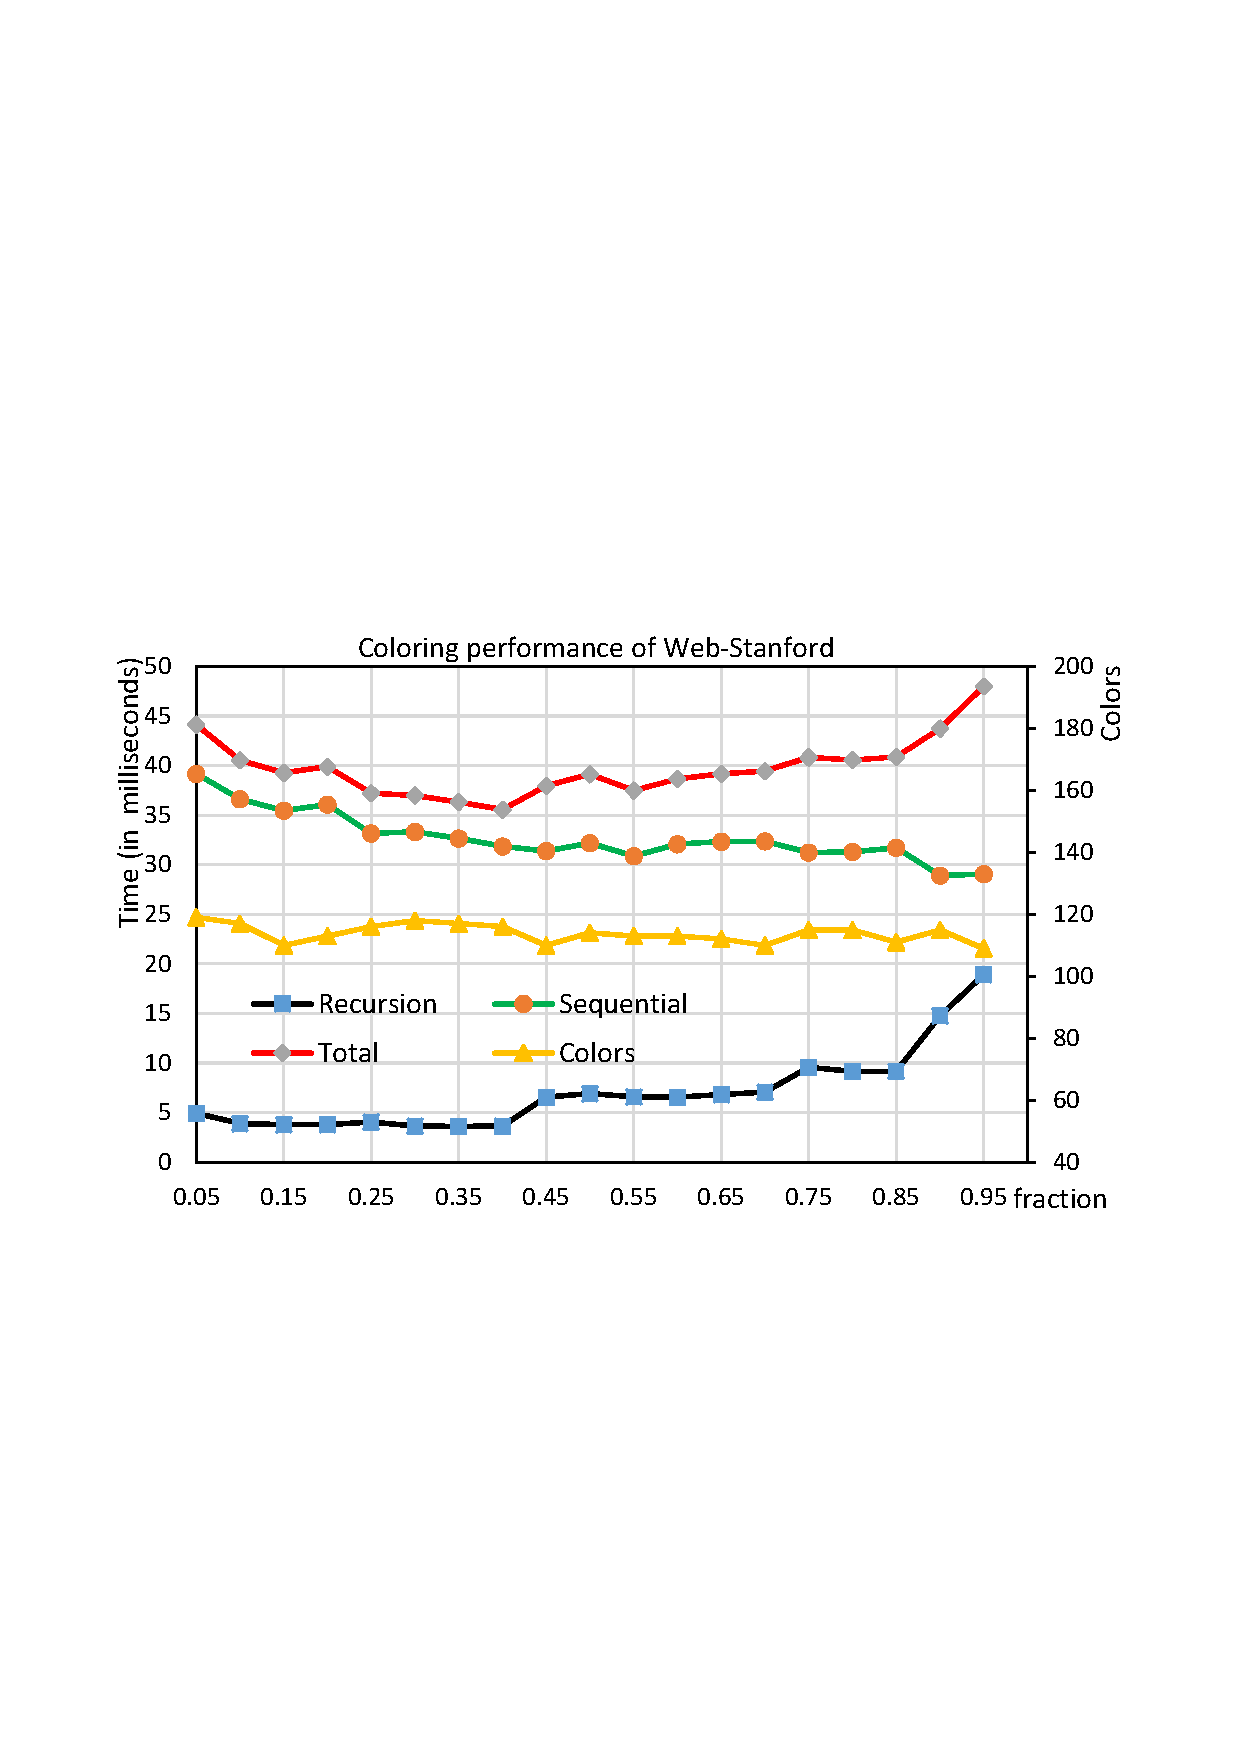
\includegraphics[scale=0.2]{figure/exp/web-s.pdf}
	}
	\subfloat[DBLP]{
		\label{fig:dblp}
		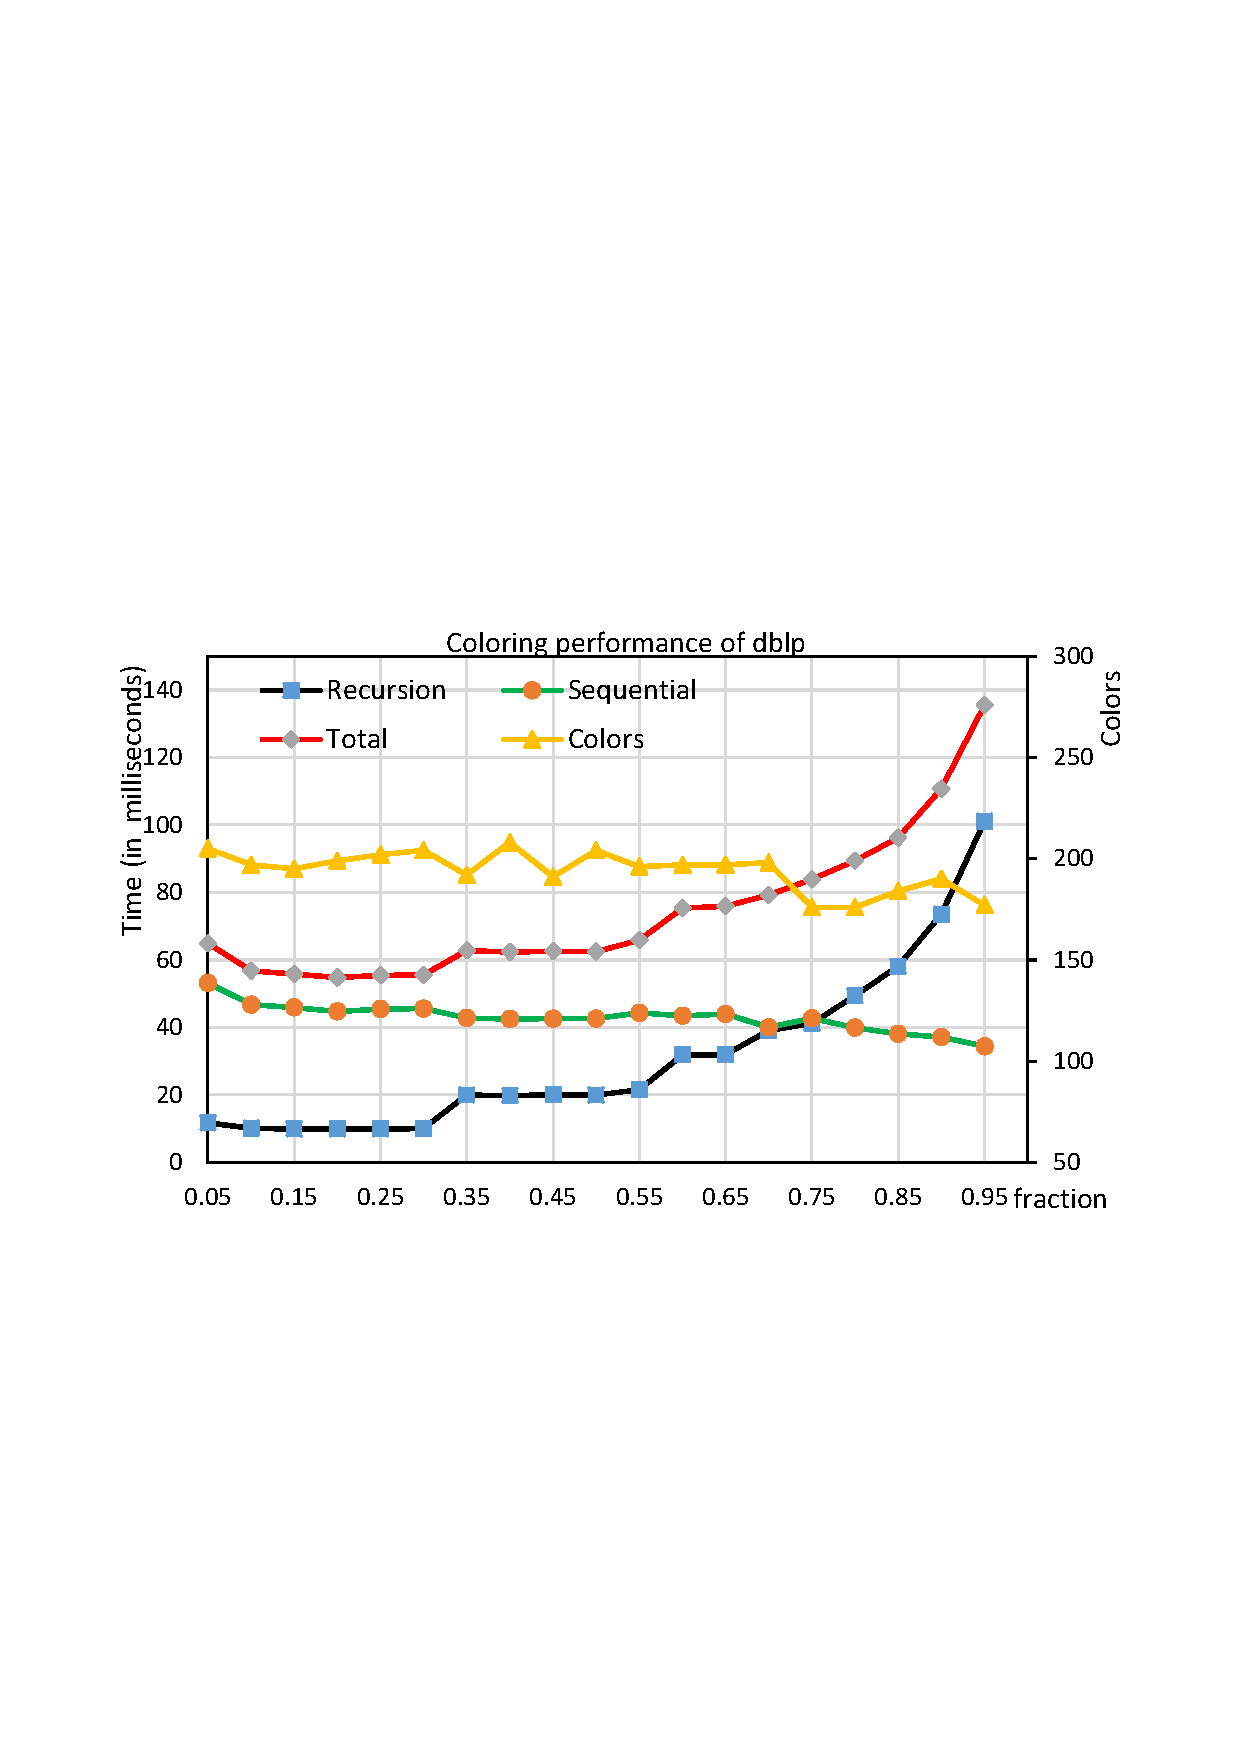
\includegraphics[scale=0.2]{figure/exp/dblp.pdf}
	} 
	\subfloat[Youtube]{
		\label{fig:youtube}
		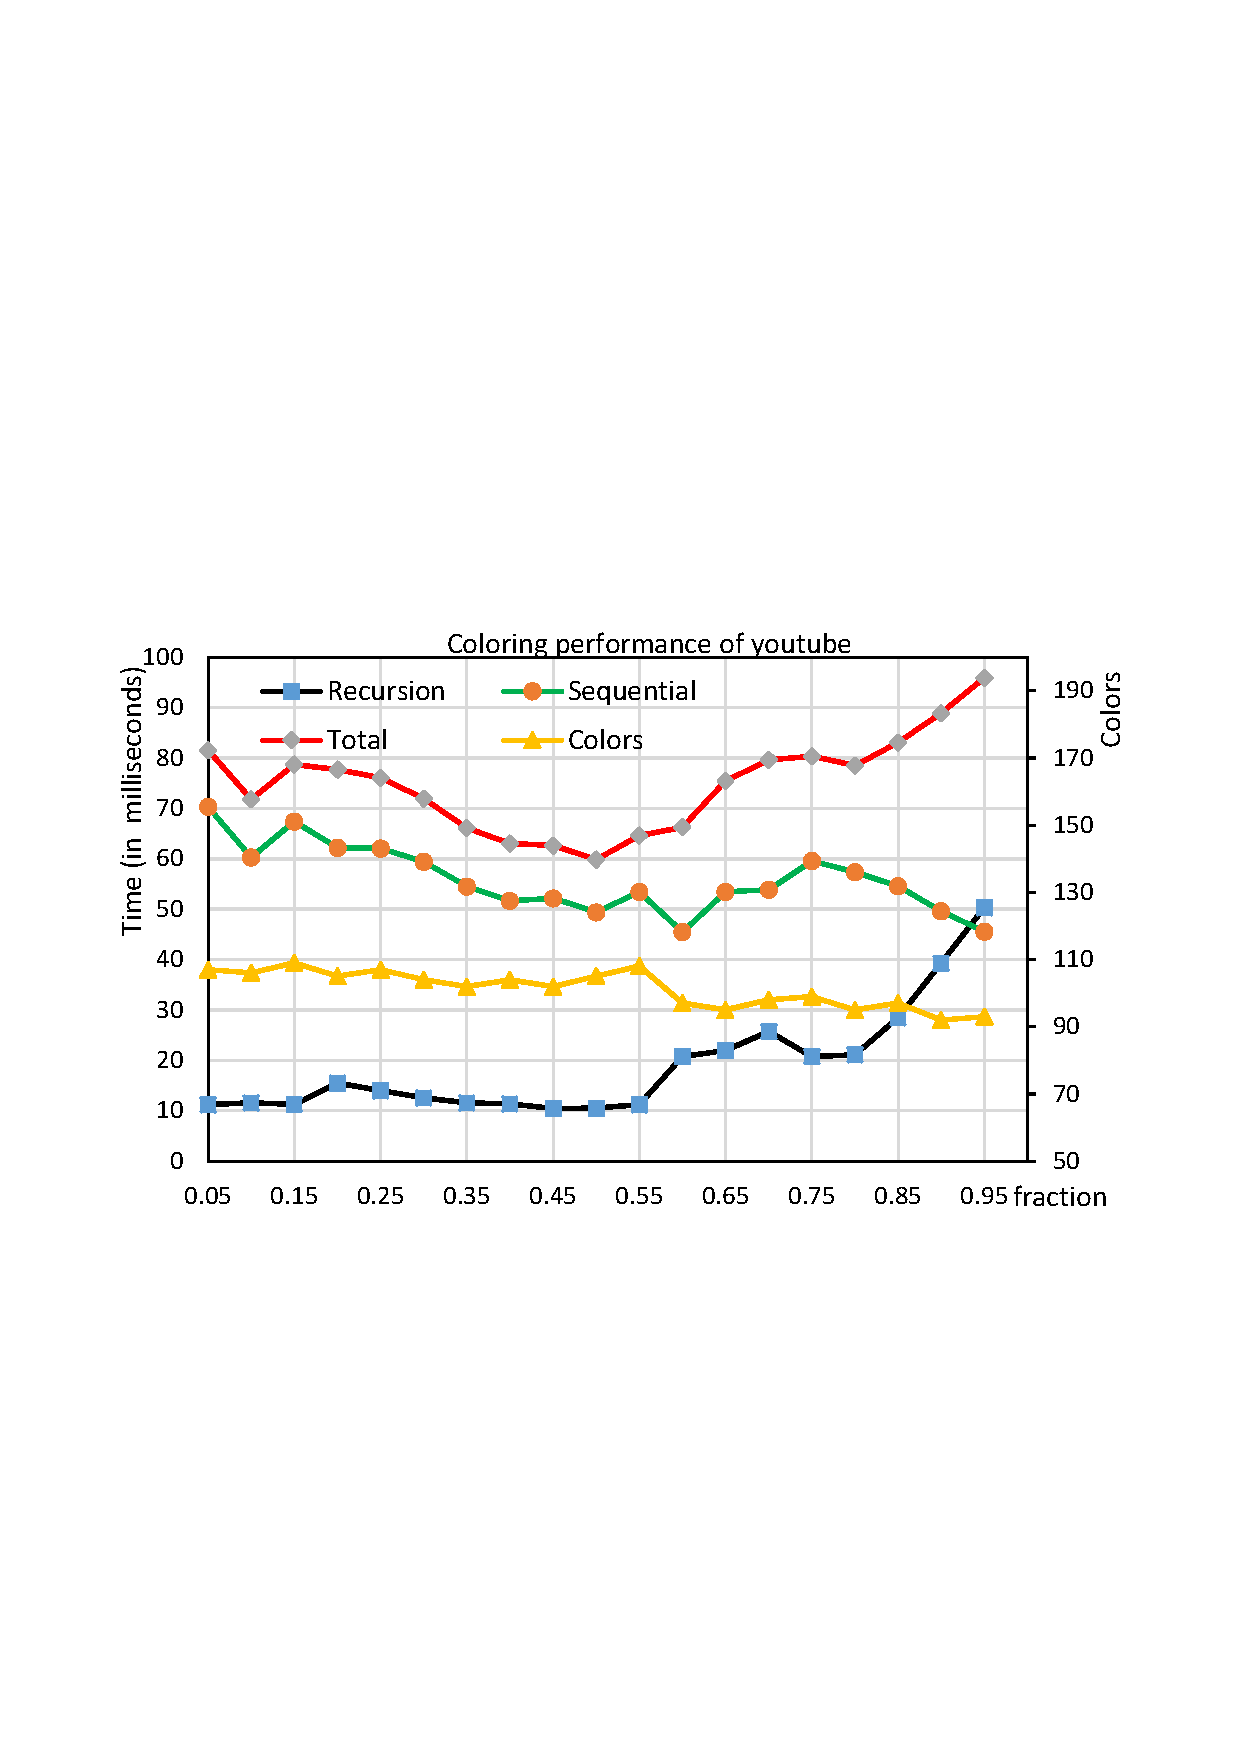
\includegraphics[scale=0.2]{figure/exp/youtube.pdf}
	}
	\subfloat[RoadNet]{
		\label{fig:roadnet}
		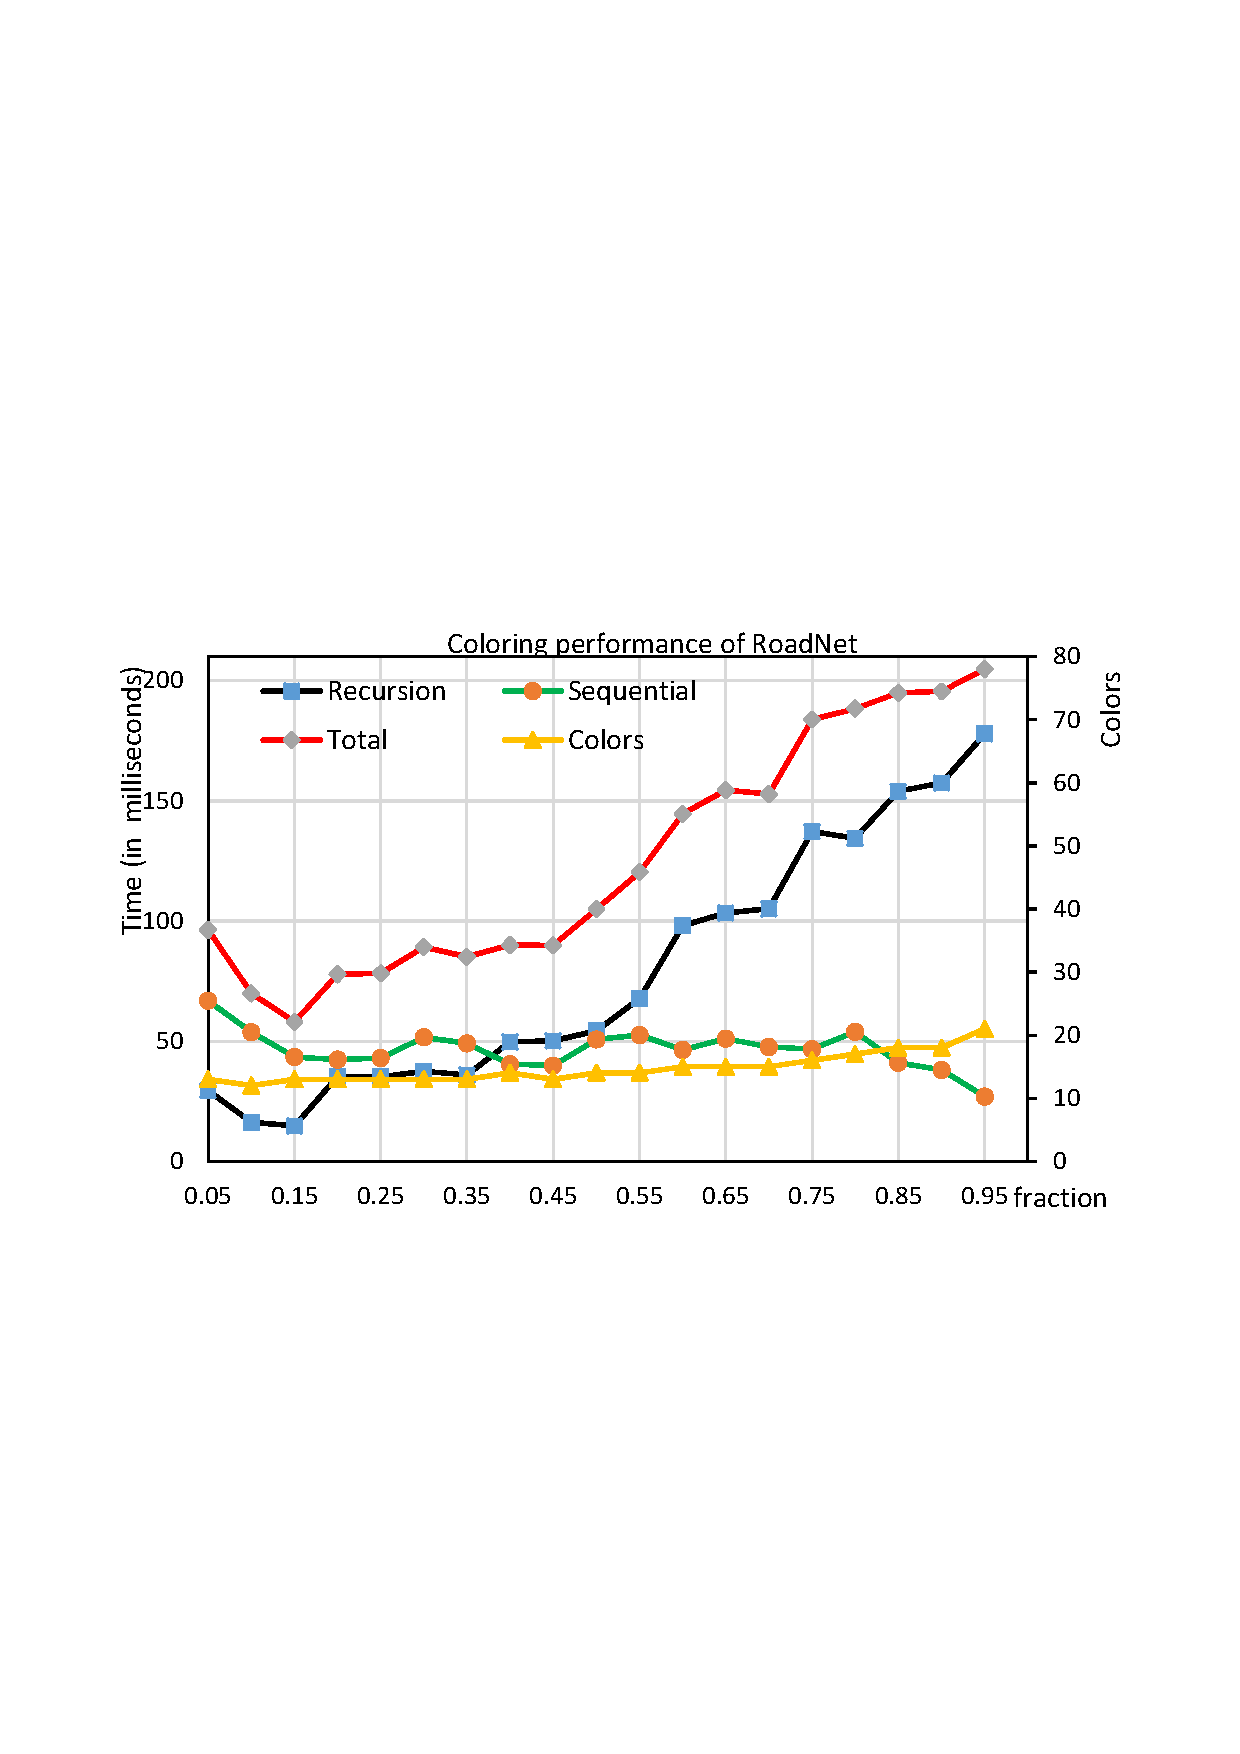
\includegraphics[scale=0.2]{figure/exp/roadnet.pdf}
	}
	\subfloat[Wiki]{
		\label{fig:wiki}
		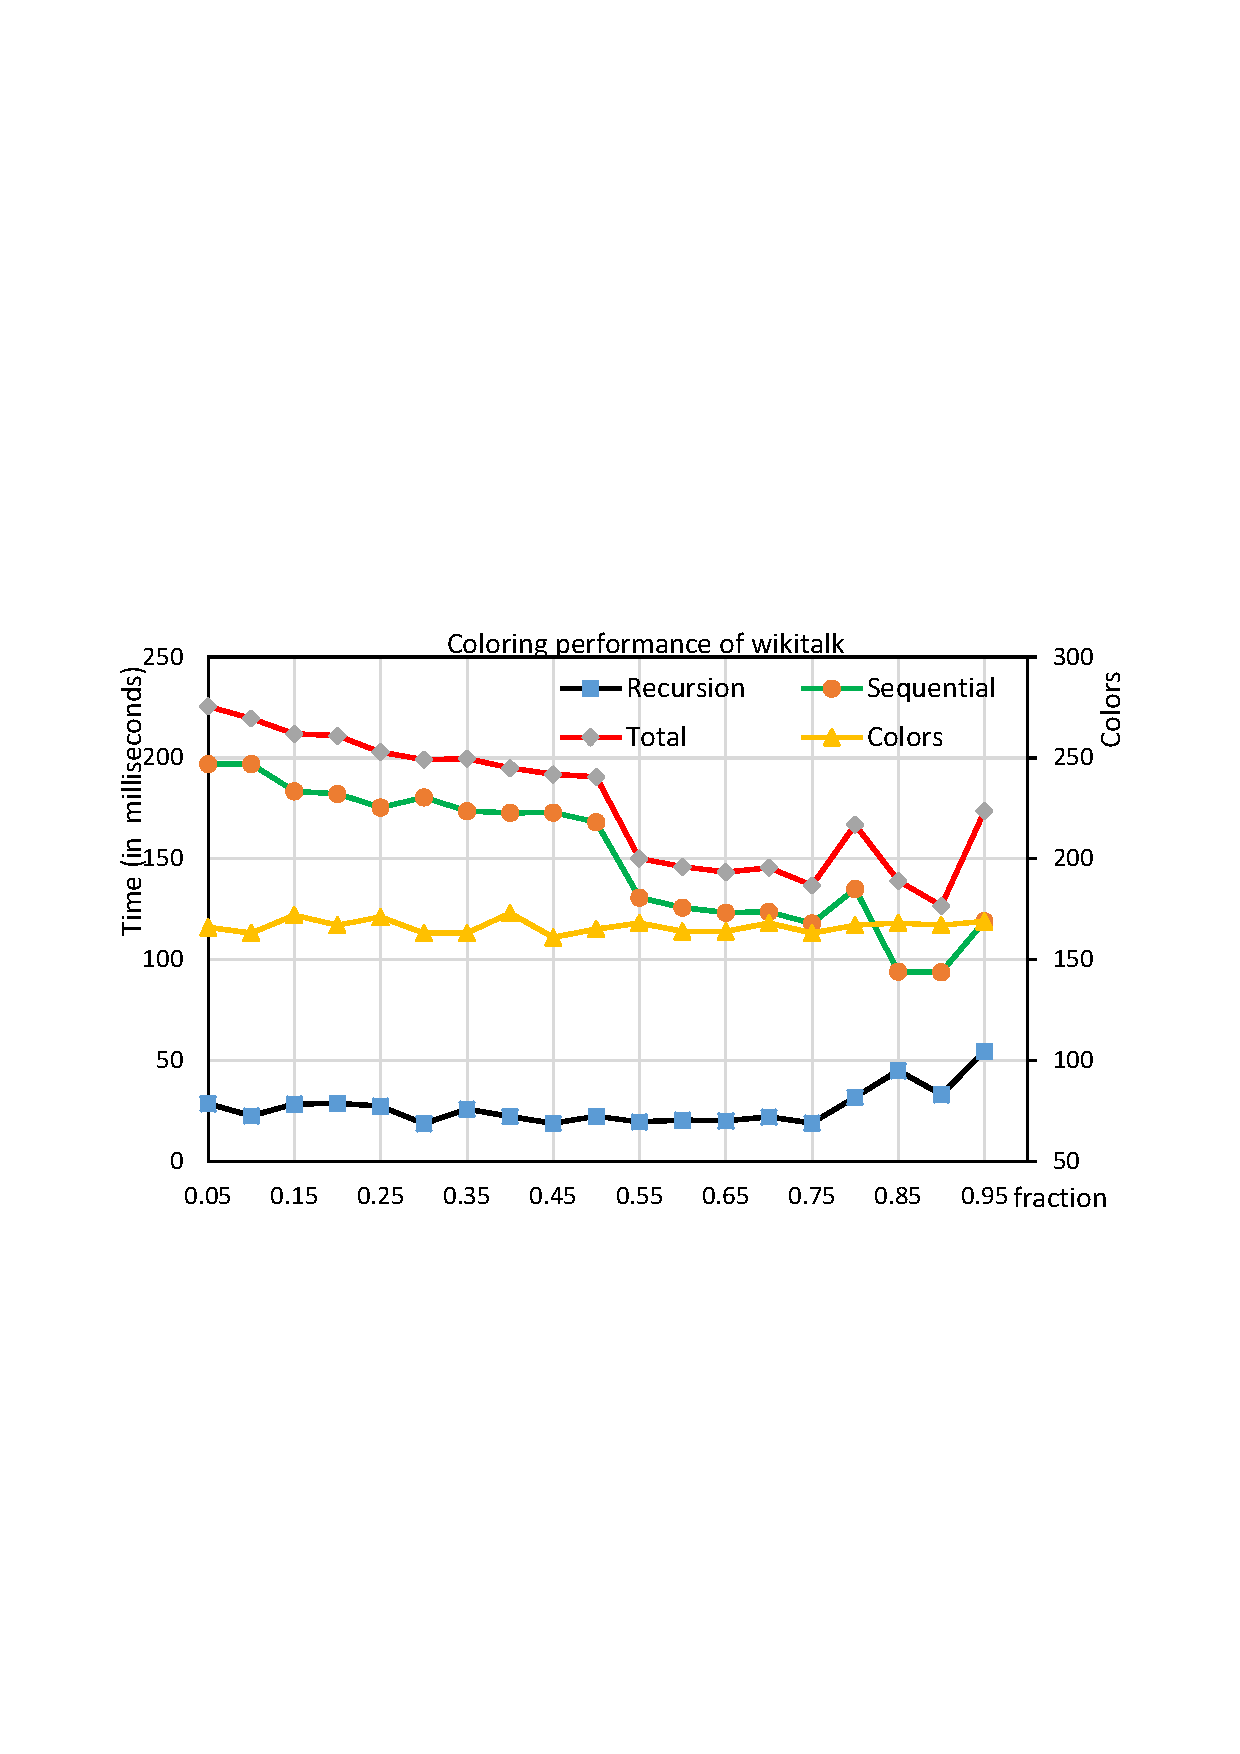
\includegraphics[scale=0.2]{figure/exp/wiki.pdf}
	}\\
	\subfloat[LiveJournal]{
		\label{fig:livejournal}
		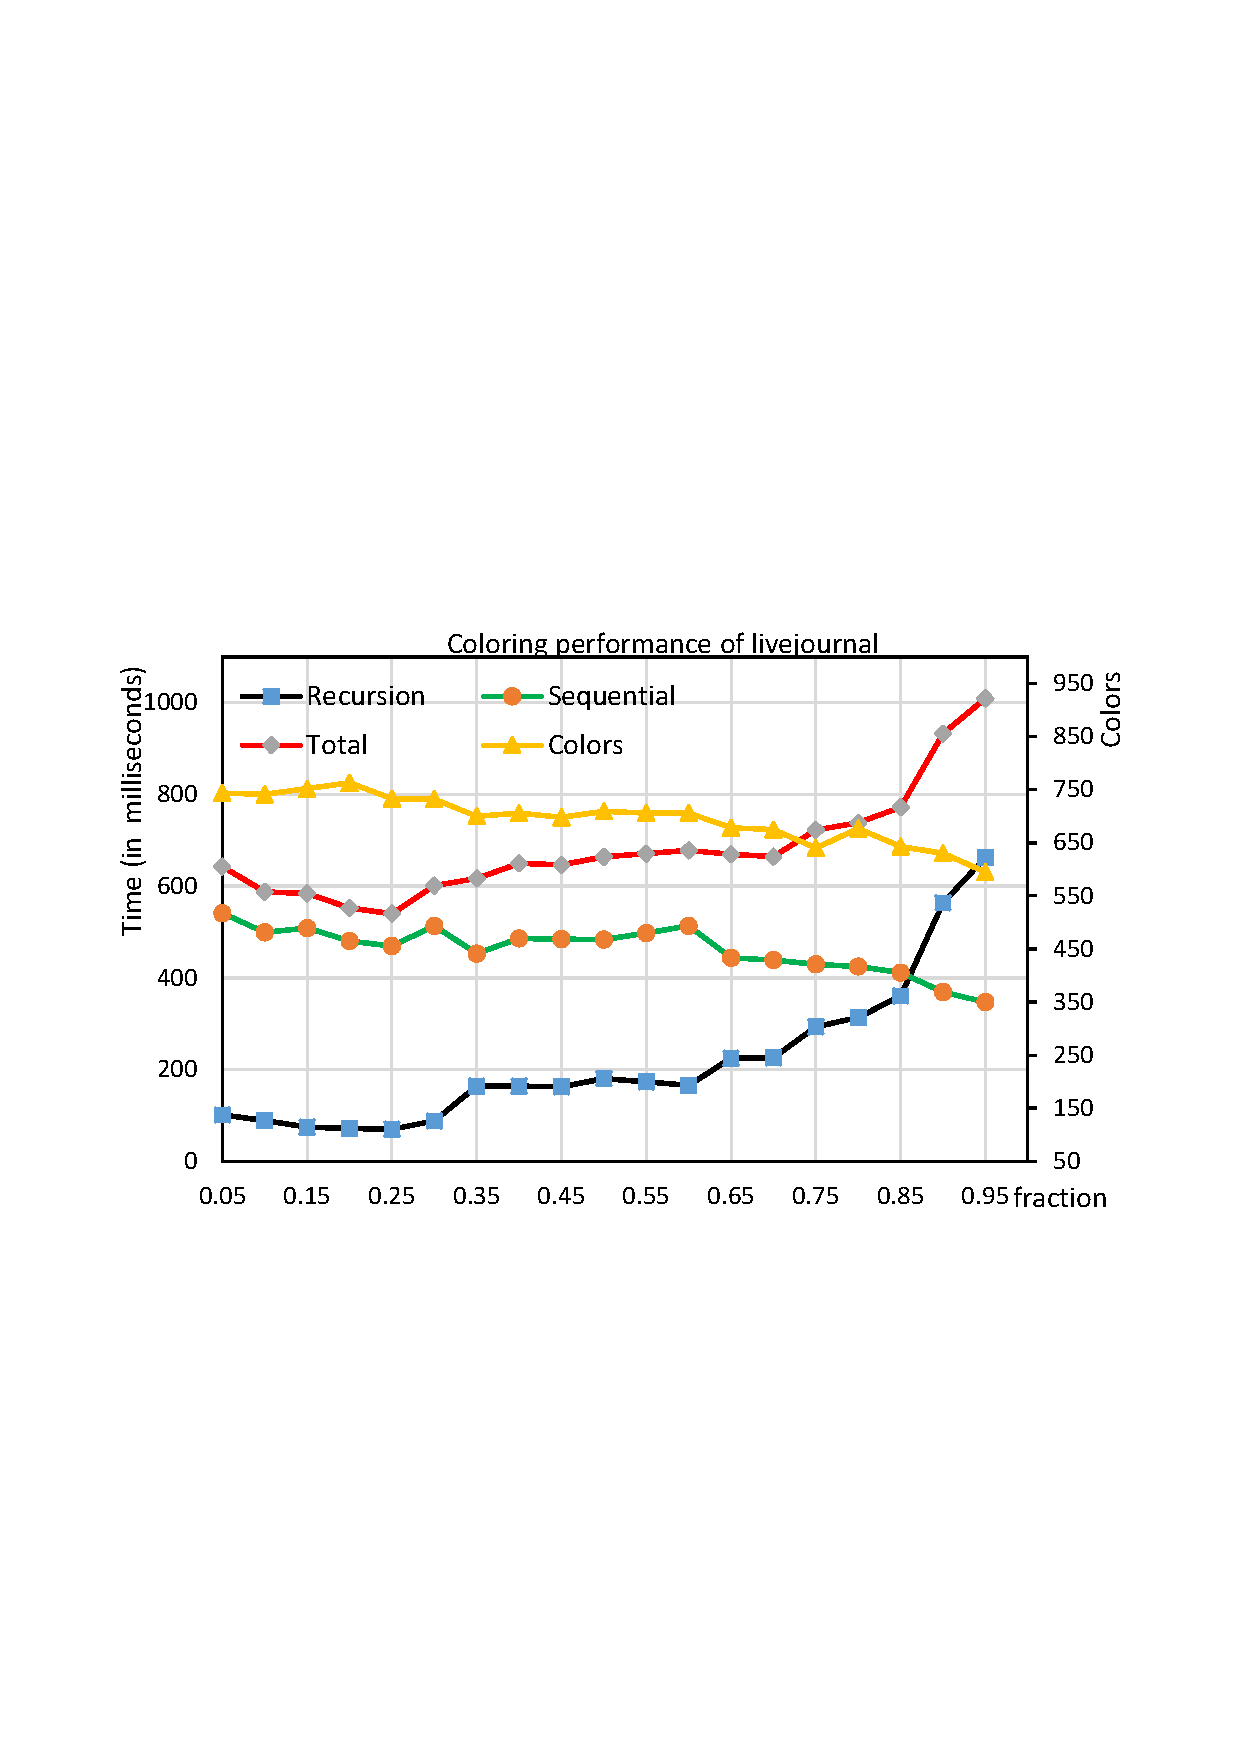
\includegraphics[scale=0.2]{figure/exp/livejournal.pdf}
	}
	\subfloat[RMAT]{
		\label{fig:rmat}
		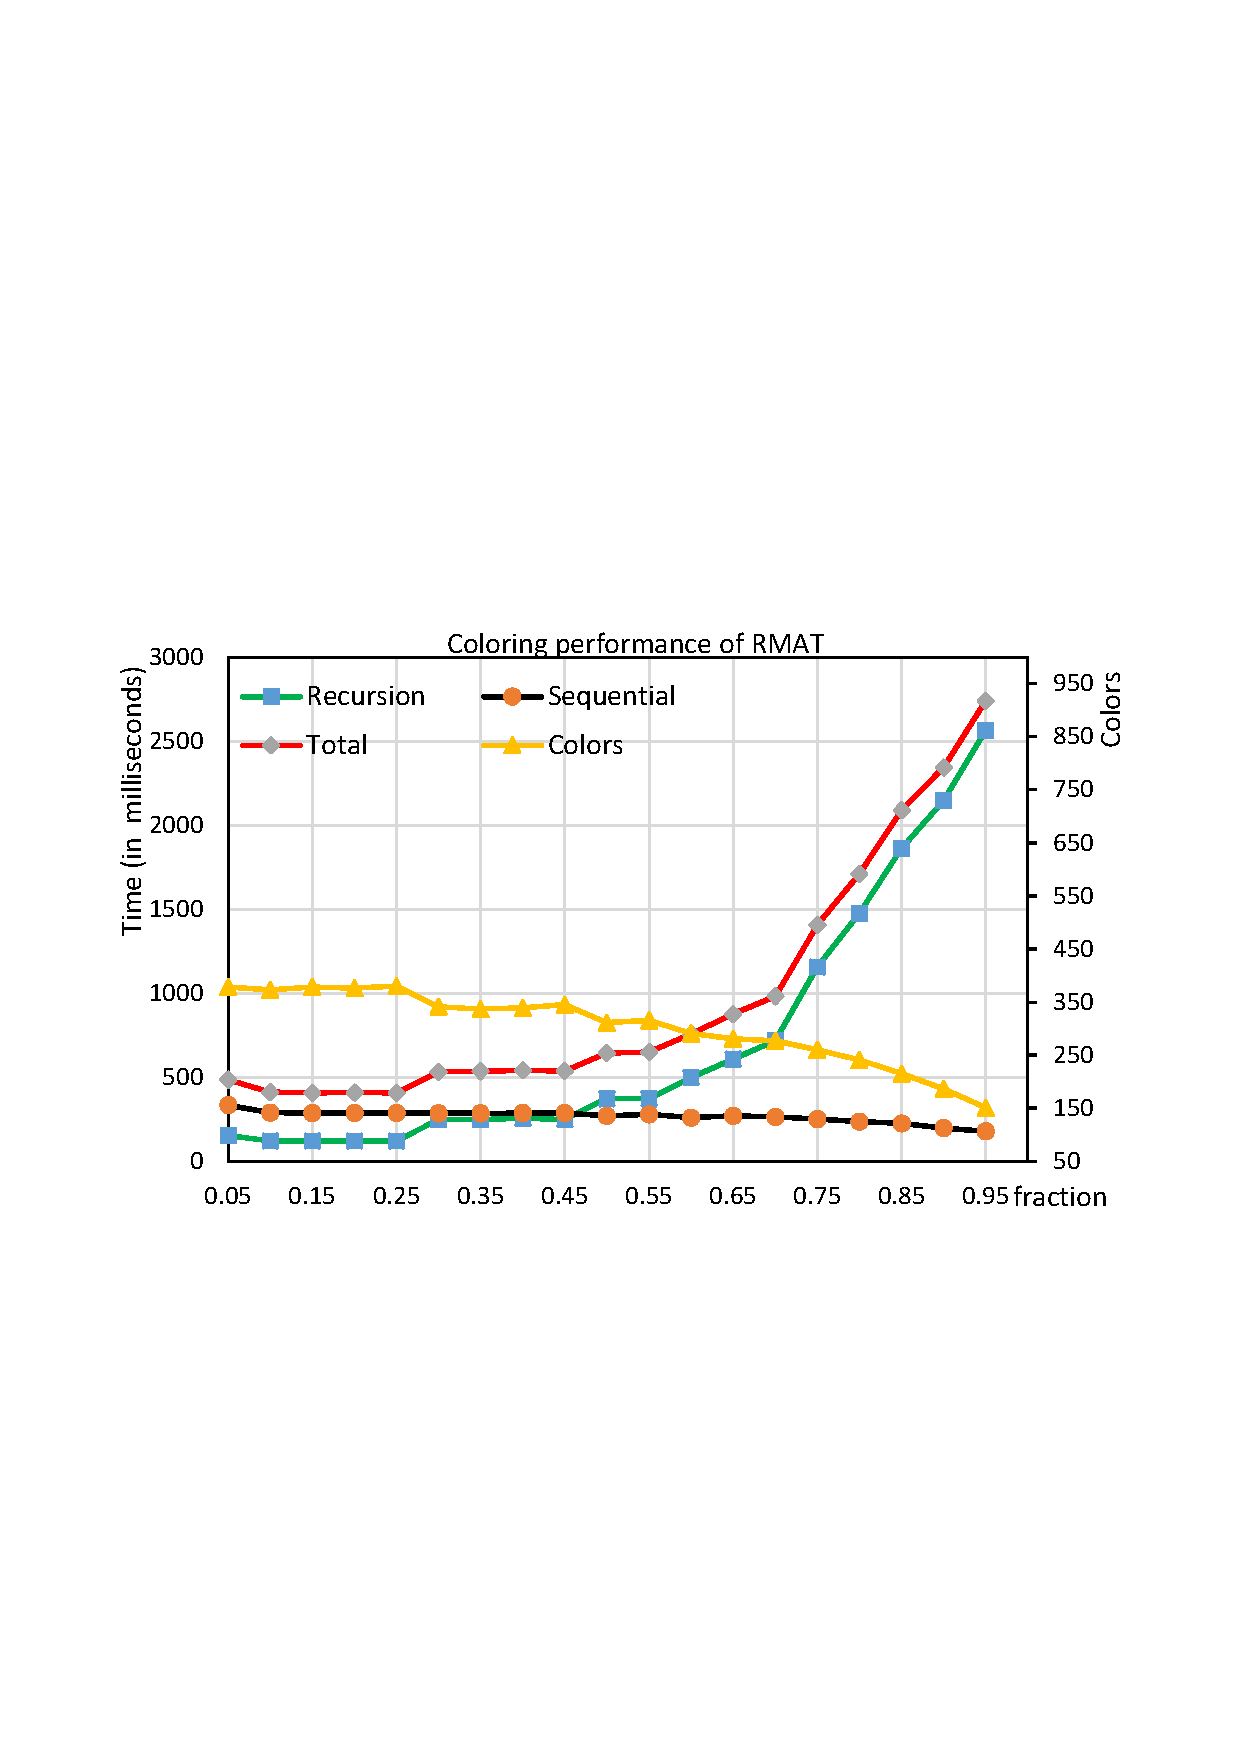
\includegraphics[scale=0.2]{figure/exp/rmat.pdf}
	}%
	\subfloat[RandomGraph]{
		\label{fig:random}
		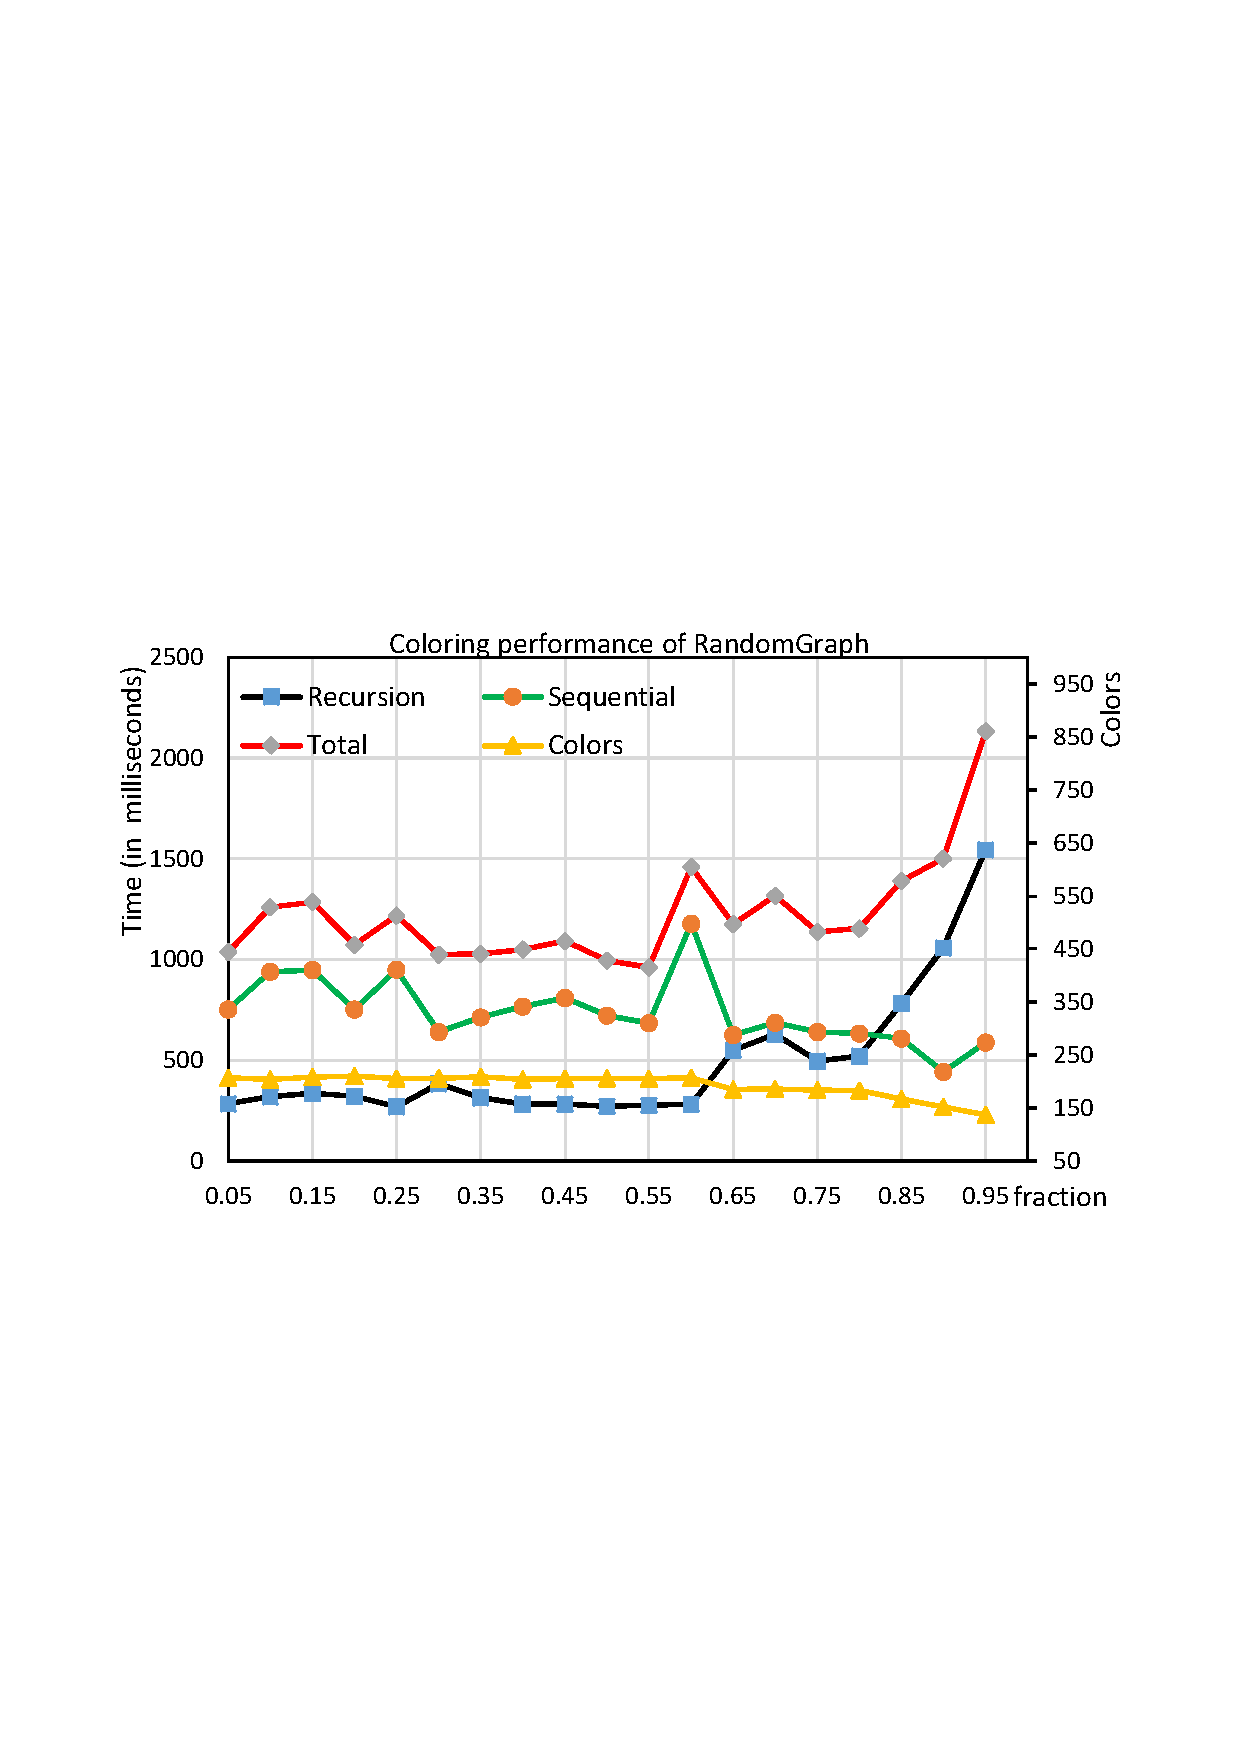
\includegraphics[scale=0.2]{figure/exp/random.pdf}
	}
	\subfloat[Twitter]{
		\label{fig:twitter}
		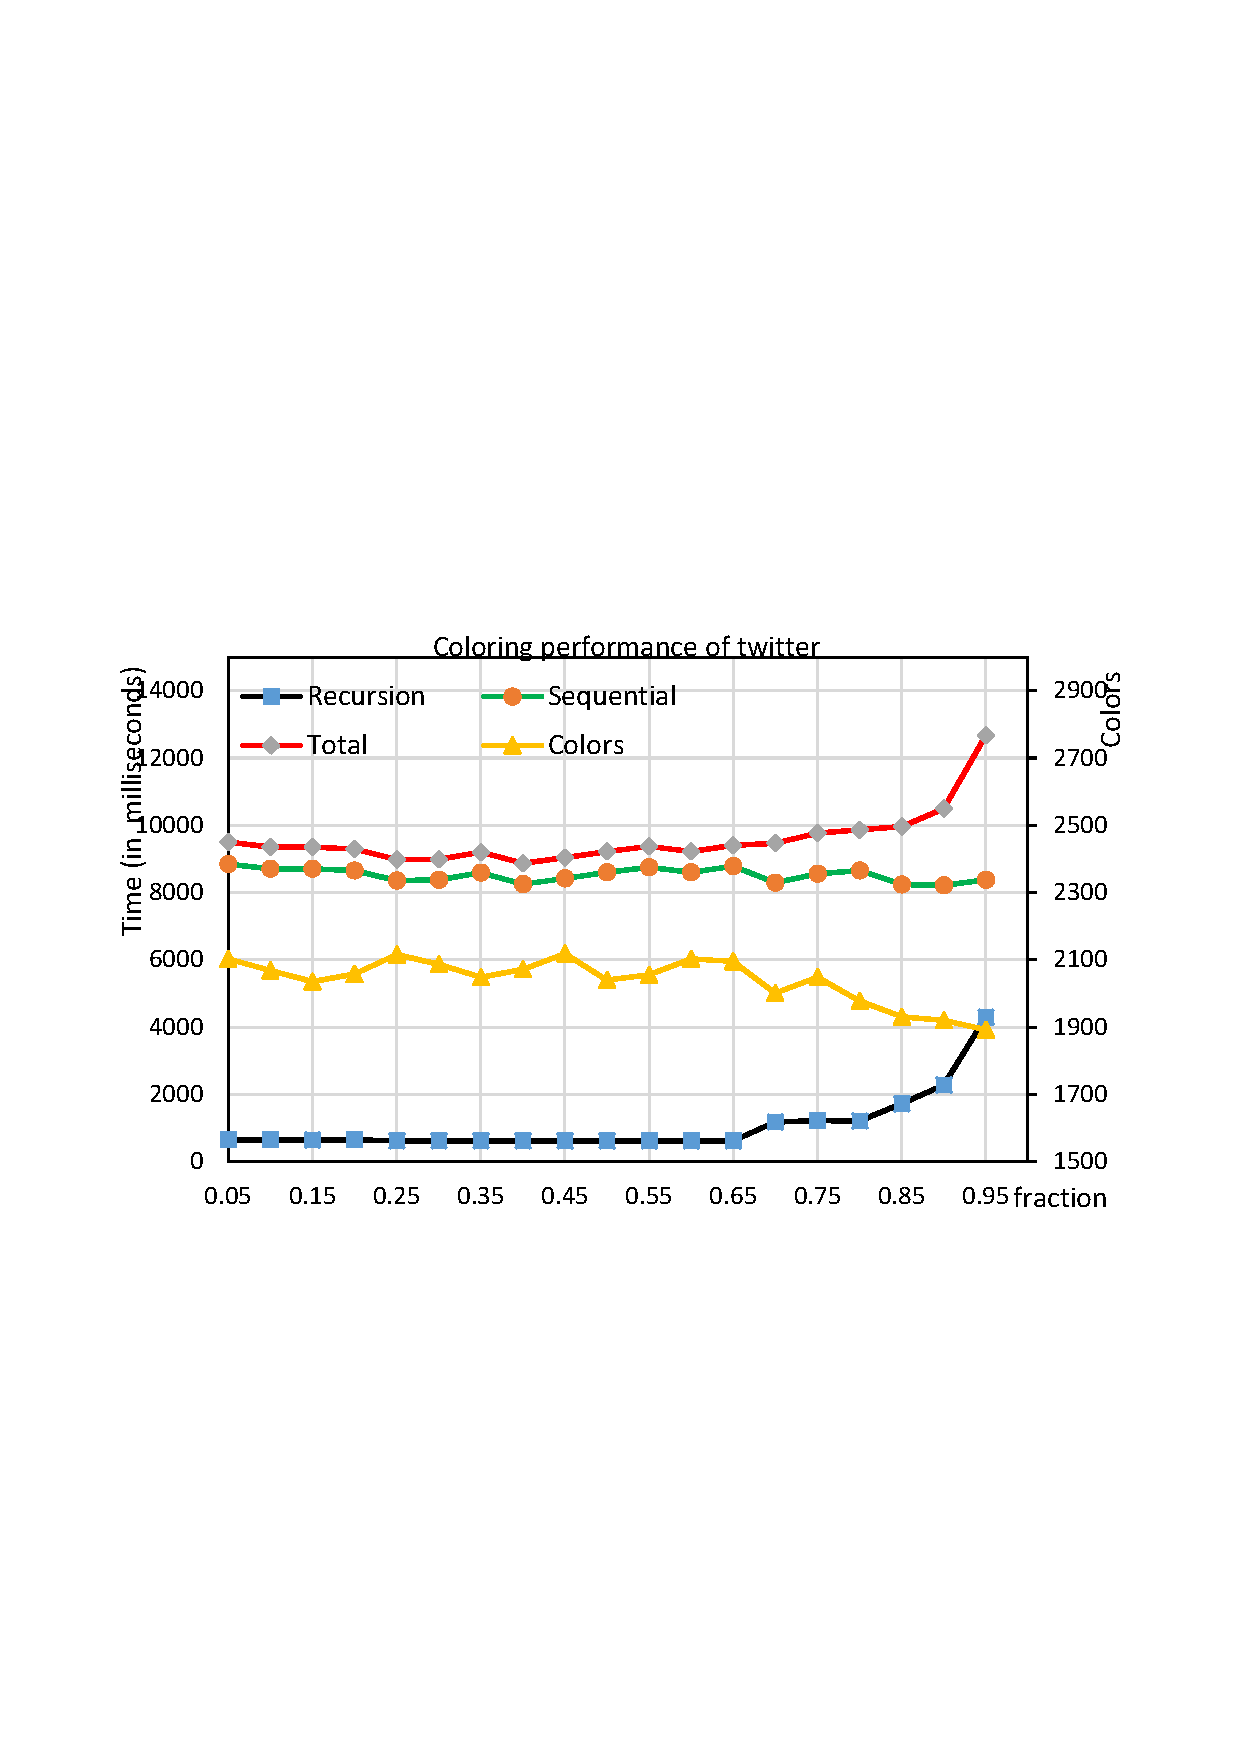
\includegraphics[scale=0.2]{figure/exp/twitter.pdf}
	}%
	\subfloat[Webbase]{
		\label{fig:webbase}
		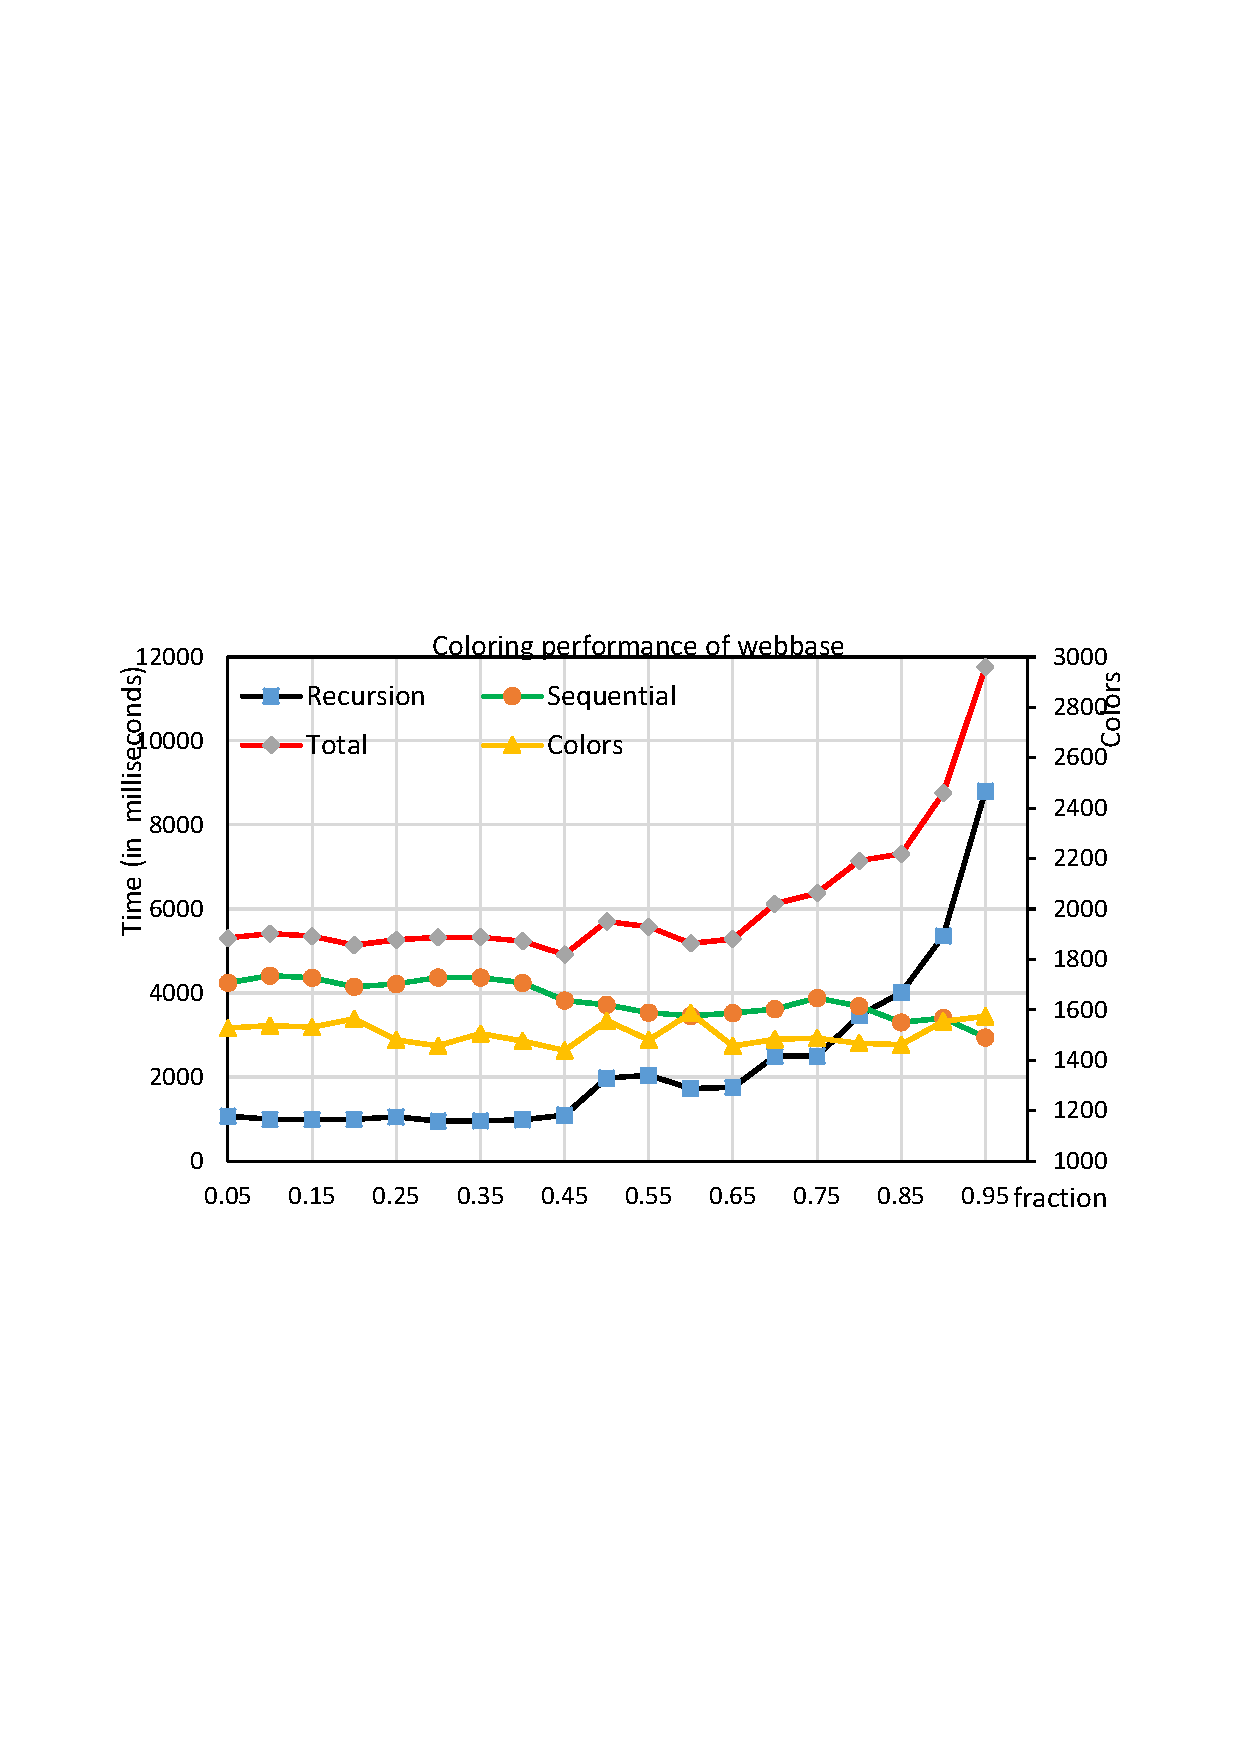
\includegraphics[scale=0.2]{figure/exp/webbase.pdf}
	}
	\caption{Coloring time with different \emph{fraction}. 
		X-axis is the value of \emph{fraction} and the Y-axis is the coloring time in milliseconds. Sequential Part means the time spent by the sequential spread stage of the coloring algorithm while the recursion part means the time by the recursion stage. The parameter \emph{fraction} indicates the ratio of the number of colored vertices in the recursion stage to the number of total vertices in the graph.}
	\label{fig:coloring}
\end{figure*}

In order to find a suitable value of the parameter $fraction$, which is used to control when the execution of Feluca is switched from the recursion stage to the sequential spread stage, we designed a set of experiments for different datasets with different value of fractions. The execution time of these two stages in Feluca with different \emph{fraction} values are shown in figure \ref{fig:coloring}. The left side y-axis in figure \ref{fig:coloring} is the coloring time in milliseconds, while the y-axis at the right side is the number of colors. The red line with gray diamond dots shows the total coloring time of Feluca, while the black line and the green line show the coloring times of the recursion and the sequential spread stage, respectively. The number of colors is shown by the yellow line with triangle dots.

We can make the following observations from figure \ref{fig:coloring}.
\begin{enumerate}
	\item The sequential spread stage is most time consuming with a small $fraction$ value, which means there are very few vertices colored in the recursion stage. According to the definition in section \ref{two-stage}, $\lambda = \frac{\sum_{j=1}^i{N_j}}{N}$ is the coloring rate in the recursion stage. When $\lambda \leq fraction =0.5$, it means there are a half vertices colored in the recursion stage while the other half are colored in the sequential spread stage. Figure \ref{fig:coloring} shows that the execution time of the recursion stage is much smaller than that of the sequential spread stage with all the power-law graphs, which means the recursion algorithm is much faster than the sequential spread algorithm. On the contrary, the recursion method needs more time with a big $fraction$ value, which means there are more conflicts occurred at the end of the  recursion stage.
	\item Feluca can achieve good performance on both power-law graphs and random graphs with a small number of colors.	
	\item Figure \ref{fig:coloring} shows that the execution time of Feluca is a convex function over $fraction$. Hence, Feluca can achieve the best coloring time when the derivative of the execution time function is close to 0. The derivative of the execution time function can be approximated as $\Delta t = \frac{t_i - t_{i-1}}{fraction_i - fraction_{i-1}}$. It can be assumed that the execution times of two consecutive iterations are the almost same. Then, Feluca switches from the recursion stage to the sequential spread stage when the number of active vertices is the same as the number of conflicting vertices in two consecutive iterations. 
\end{enumerate}

The recursion method becomes less efficient in in the later iterations, which is known as the long tail problem. Since Feluca assigns the colors to the conflicting vertices following the edges directions, most conflicting vertices can find suitable colors in the first few iterations. However, after a majority of vertices find the suitable colors, these colored vertices will have impact on the colors of the remaining vertices. This causes a small number of remaining vertices to change their colors repeatedly in later iterations and therefore shows down the progress. This is why Feluca switches from the recursion stage to the sequential spread stage when the condition stated in the last observation made from figure \ref{fig:coloring} is met.

\subsection{Comparison Against the State-of-the-art Techniques}

\begin{table*}[hpt]
\centering
\caption{Execution time for different coloring algorithms (in milliseconds)}
\label{tab:algs}
\begin{threeparttable}
\resizebox{\linewidth}{!}{
\begin{tabular}{|l|r|r|r|r|r|r|r|r|r|r|r|r|r|r|}
\hline
\multirow{2}{*}{Datasets} &\multicolumn{2}{c|}{CPU\_Greedy}	&\multicolumn{2}{c|}{Feluca}	&\multicolumn{2}{c|}{JPL}	&\multicolumn{2}{c|}{kokkos\_MIC}	&\multicolumn{2}{c|}{kokkos}	&\multicolumn{3}{c|}{cuSPARSE}\\ \cline{2-14} % &\multicolumn{1}{c|}{\multirow{2}{*}{Speedup}} \\ 
                  &\multicolumn{1}{c|}{Time} &\multicolumn{1}{c|}{Color}	&\multicolumn{1}{c|}{Time} &\multicolumn{1}{c|}{Color}	&\multicolumn{1}{c|}{Time} &\multicolumn{1}{c|}{Color} 	&\multicolumn{1}{c|}{Time} &\multicolumn{1}{c|}{Color}	&\multicolumn{1}{c|}{Time} &\multicolumn{1}{c|}{Color} 	&\multicolumn{1}{c|}{Time} &\multicolumn{1}{c|}{Color} &\multicolumn{1}{c|}{\tabincell{l}{Incorrect \\ Vertices}}\\ \hline%		&\multicolumn{1}{c|}{}\\ \hline
 web-Stanford			&103.955					&149					&\textbf{28.810}		&92					&1121.790		&169	&2200.720		&\textbf{45}&50.765			&\textbf{45}	&1463.250					&95						&134993\\
 dblp							&322.065					&119					&\textbf{42.388}		&139				&787.762		&121	&6106.440		&119				&183.034		&119					&541.429					&\textbf{70}	&933161\\
 youtube					&216.808					&\textbf{43}	&\textbf{58.777}		&57					&1409.490		&262	&3022.930		&46					&230.806		&45						&617.205					&103					&283515\\
 RoadNet					&145.619					&\textbf{5}		&\textbf{12.524}		&6					&806.787		&13		&4893.600		&5					&162.546		&6						&531.205					&32						&1953477\\
 Wiki-Talk				&774.658					&97						&\textbf{122.464}		&95					&8703.570		&489	&5042.670		&67					&631.069		&\textbf{65}	&818.762					&159					&184167\\
 soc-LiveJournal	&4805.730					&328					&\textbf{448.574}		&551				&11000.500	&646	&63284.500	&251				&1629.902		&251					&1792.390					&\textbf{184}	&2437231\\
 RMAT16\_2				&8965.460					&75						&\textbf{485.550}		&410				&18774.900	&316	&163517			&26					&4454.264		&\textbf{23}	&6910.610					&129					&6966819\\
 random-graph			&9076.560					&94						&\textbf{353.643}		&86					&17264.300	&334	&96557.300	&25					&2968.788		&\textbf{22}	&9264.060					&112					&4804572\\
 twitter-2010			&83796.800				&918					&\textbf{5040.660}	&947				&null				&null	&728099			&\textbf{679}&null			&null					&41201.3					&917	&22396212\\
 webbase-2001			&343404						&1507					&\textbf{2729.500}	&1559				&null				&null	&940540			&1226				&null			&null						&264022						&\textbf{412}	&104173619\\\hline
 Feluca Speedup		&\multicolumn{2}{c|}{3.61$\times$ -- 125.81$\times$}	&\multicolumn{2}{c|}{--}			&\multicolumn{2}{c|}{18.58$\times$ -- 71.07$\times$}		&\multicolumn{2}{c|}{41.18$\times$ -- 344.58$\times$} &\multicolumn{2}{c|}{1.76$\times$ -- 12.98$\times$}	&\multicolumn{3}{c|}{4$\times$ -- 96.73$\times$}\\\hline
\end{tabular}}
\begin{tablenotes}
\item {Note: }{Null means that the system cannot process such a dataset. CPU\_Greedy and kokkos\_MIC are run on the Intel(R) Xeon(R) \\ 
E5-2670 CPU with 16 threads, while others are run on \texttt{NVIDIA Tesla K20m GPU}. Reference \cite{Manycore} shows that kokkos can achieve the \\ 
best performance by using the edge-based coloring method. So we set the parameter \texttt{--algorithm} as \texttt{COLORING\_EB} for kokkos\_MIC \\
and kokkos in our experiments. 
%We also tried to run kokkos on \texttt{NVIDIA Tesla K20m GPU}, but failed. This may be due to the flaw in kokkos since the authors said ``sometimes the build system acts weird especially when configure options are changed''.
}
%\item {GPU. And the improvement is made based on Frog.}
\end{tablenotes}
\end{threeparttable}
\end{table*}

We compared Feluca with some recent researches, such as cuSPARSE, JPL ~\cite{nvidiaTR} and a CPU implementation of greedy coloring algorithm. Table \ref{tab:algs} shows the execution time and the number of colors used for all ten graphs. A performance value plotted in each graph is the average of 5 independent runs of the GPU-based solutions (Feluca, cuSparse, and JPL) or the average of 10 runs of the CPU based implementation.

The experimental results show that Feluca achieves up to 125.81$\times$ speed up over the CPU-based Greedy coloring algorithm, 111.98$\times$ speed up over the JPL algorithm and up to 96.73$\times$ speed up over the state-of-the-art cuSPARSE algorithm. For the reference, one of the recent researches \cite{Manycore} achieved only up to 1.5$\times$ speed up over cuSPARSE. 

Table \ref{tab:algs} shows that Feluca outperforms all other competitors in terms of run-time with all ten datasets. All these algorithms can generate a complete coloring plan except cuSPARSE, which is an incomplete coloring algorithm. For example, out of the 4,847,571 vertices in \texttt{soc-LiveJournal}, 41,652,230 vertices in \texttt{twitter-2010}, 118,142,155 vertices in \texttt{webbase-2001}, cuSPARSE assigns 2,437,231 and 22,396,212 and 104,173,619 vertices, respectively, to the same color. From another point of view, cuSPARSE does not choose another right color for the vertices when the conflicts occur. 41,652,230 vertices of \texttt{twitter-2010} are colored with 947 colors in Feluca while cuSPARSE only colored the 19,256,018 (46\% of all the vertices) vertices  using 917 colors and assigns the remaining 22,396,212 vertices to the same color. This is the main reason why cuSPARSE can achieve a fewer number of colors on \texttt{soc-LiveJournal, twitter-2010} and \texttt{webbase-2001}.

As described in section \ref{eliminate}, Feluca only focuses on the current vertex and their parents and does not search the entire color array to find the available color for the current vertex. Although this scheme avoids the use of atomic operations (hence improve the run-time performance), it may increase the number of used colors to some extent. Table \ref{tab:algs} shows cuSPARE can color the \texttt{soc-LiveJournal}, \texttt{twitter-2010} and \texttt{webbase-2001} datasets with the fewer colors than Feluca. The smaller color count by cuSPARSE is also due to incomplete nature of its solution. 

\subsection{The Color-centric Scheme in Feluca}
\label{perfo}

In this experiment, we implement Feluca with and without the color-centric paradigm. The experiment is designed to show the ratio of the number of conflicting vertices to the number of active vertices in each iteration. The experiment result is shown in figure \ref{fig:scale}. The figure shows that, without the color-centric paradigm the tested three datasets, \texttt{web-Stanford}, \texttt{youtube} and \texttt{RandomGraph}, need at least 24 iterations to converge. While with the color-centric paradigm, \texttt{RandomGraph} converged at the $7^{th}$ iteration and other two datasets converged at the $11^{th}$ iteration.

Figure \ref{fig:scale} also shows that with the color-centric paradigm, the ratio of the number of conflicting vertices to the number of active vertices in each iteration is no more than 45\% for \texttt{youtube} and \texttt{RandomGraph}, while the conflict ratio can increase to 80\% -- 87\% without the color-centric paradigm. The color-centric paradigm can avoid about 50\% conflicts for these two datasets. The conflict ratio of \texttt{web-Stanford} increased to 87\% at the $10^{th}$ iteration, while the conflict ratio is no more than 63\% with the color-centric paradigm.

\begin{figure}[h]
	\centering
		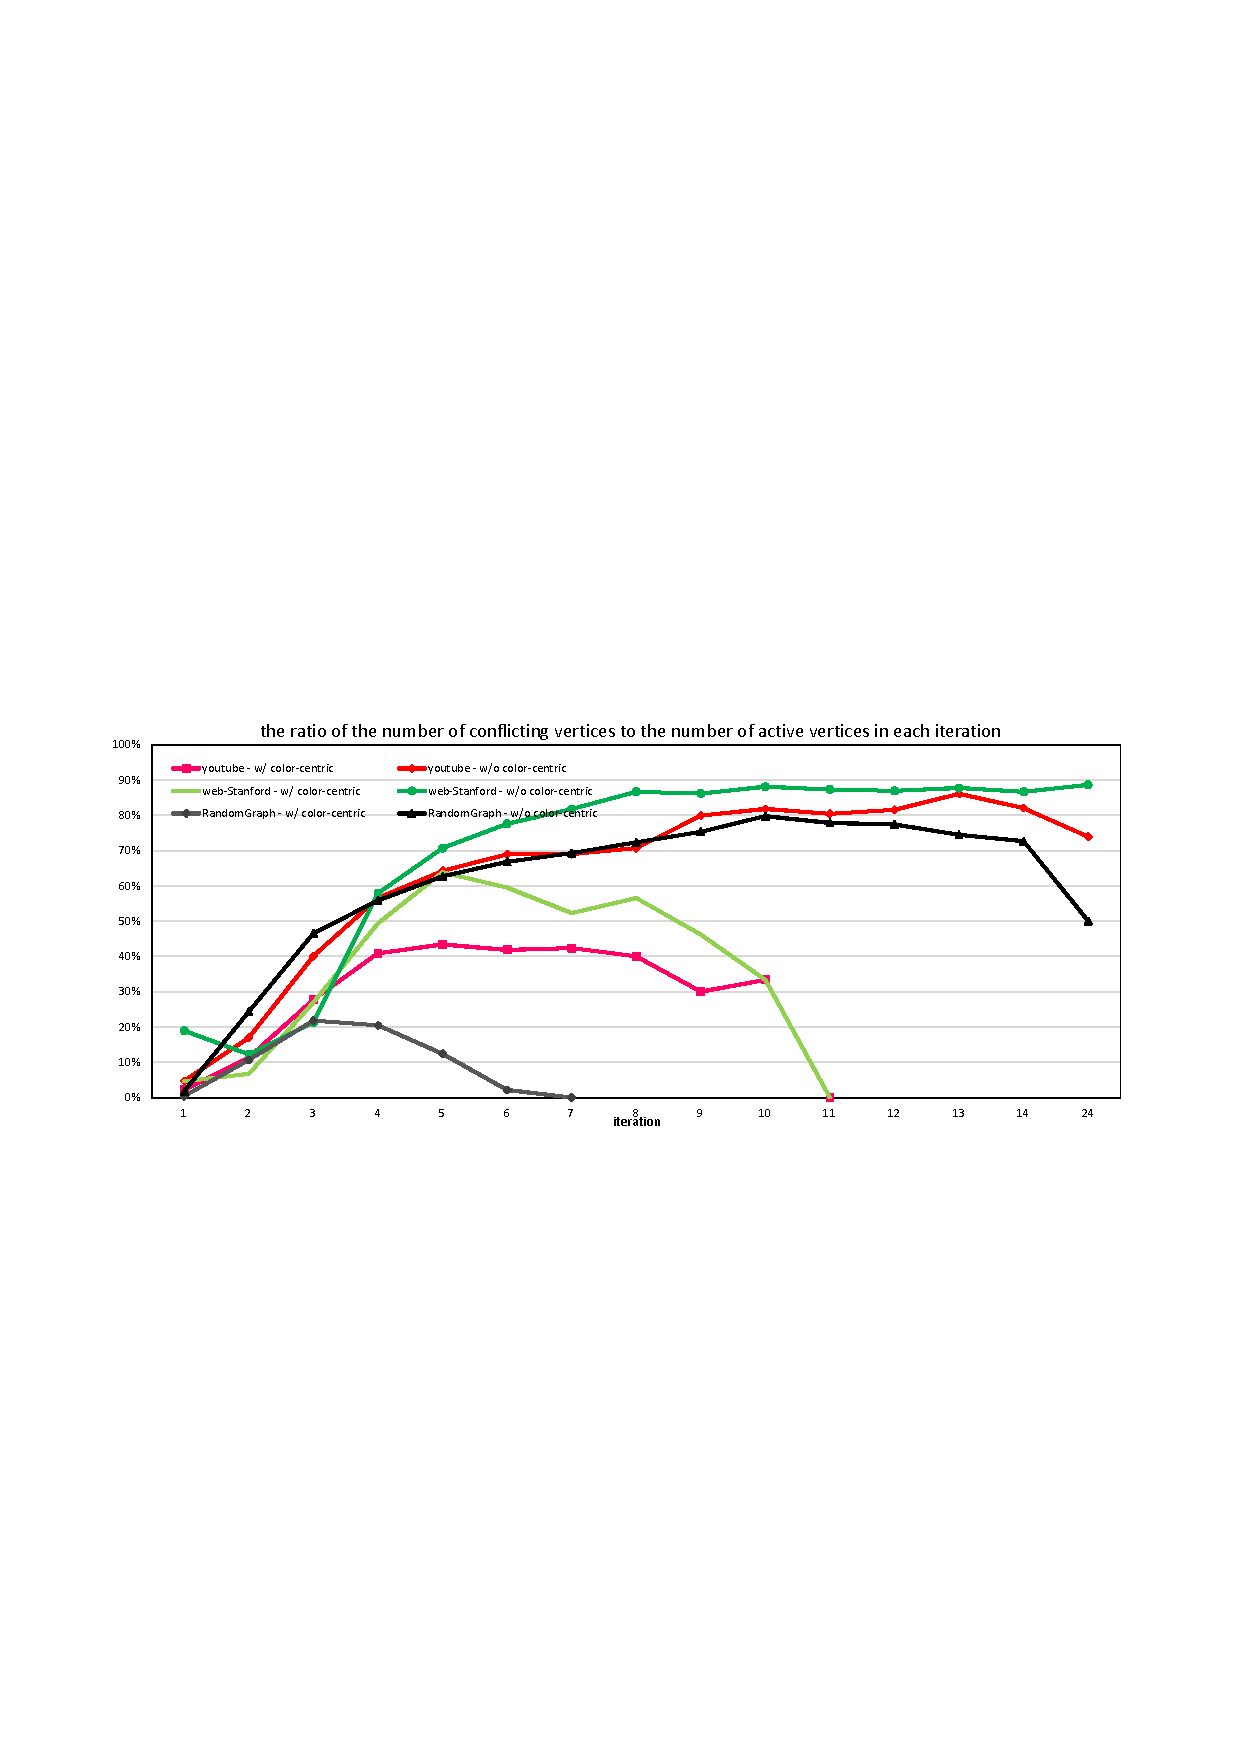
\includegraphics[scale=0.4]{figure/conflict_Feluca.pdf}
	\caption{The ratio of the number of conflicting vertices to the number of active vertices in each iteration with and without color-centric optimization}
	\label{fig:scale}%
\end{figure}

\begin{figure}[h]
	\centering
		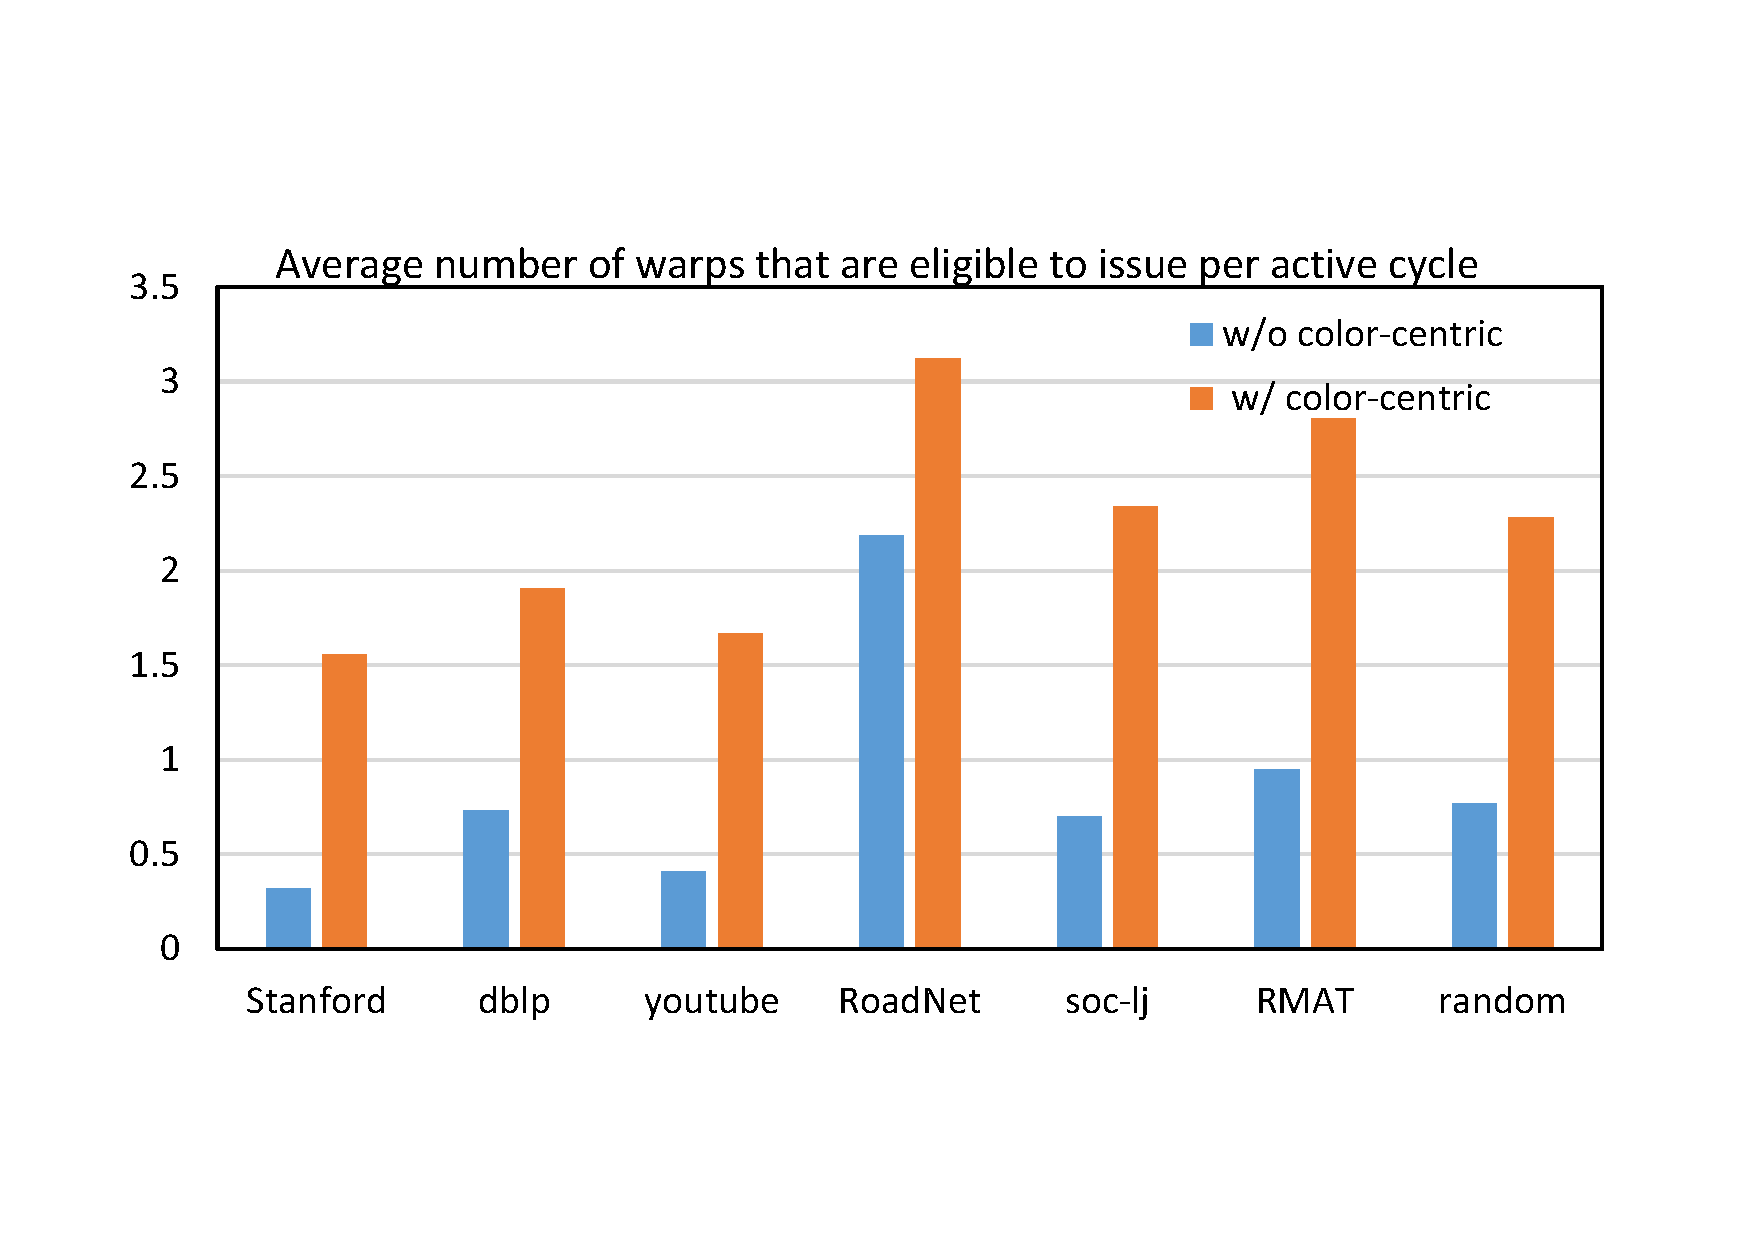
\includegraphics[scale=0.25]{figure/exp/warps.pdf}
	\caption{The average number of warps that are eligible to issue per active cycle with and without color-centric optimization}
	\label{fig:warps}%
\end{figure}

Figure \ref{fig:slot_utilization} shows the percentage of issue slots that issued at least one instruction, averaged across all cycles. The figure shows that the color-centric paradigm can improve the performance by 111\% (on RoadNet dataset) -- 410\% (on web-Stanford dataset), which indicates that more instruction were executed in every iteration by using the color-centric paradigm.

\begin{figure}[h]
	\centering
		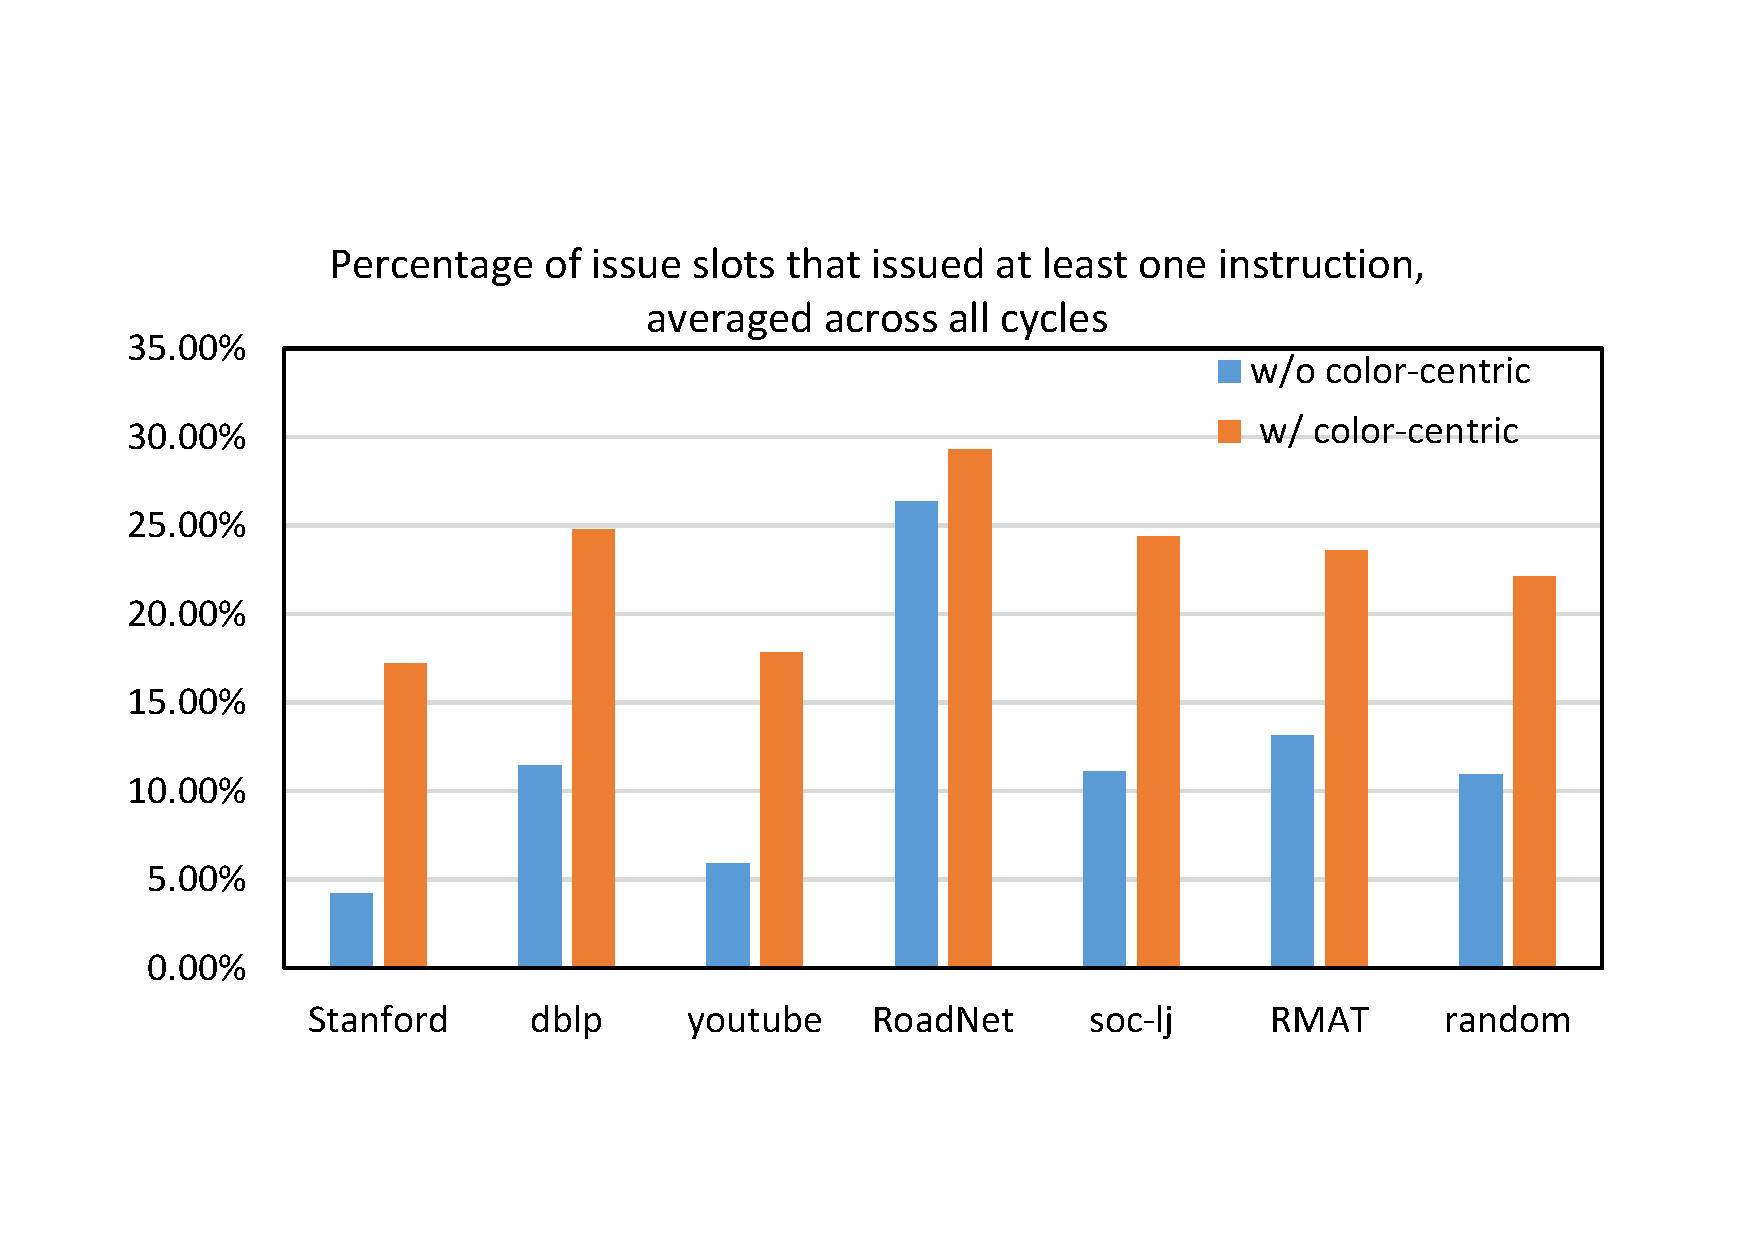
\includegraphics[scale=0.25]{figure/exp/slot_utilization.pdf}
	\caption{The percentage of issue slots that issued at least one instruction, averaged across all cycles, with and without the color-centric scheme}
	\label{fig:slot_utilization}%
\end{figure}

Figure \ref{fig:warps} plots the average number of warps that are eligible to issue per active cycle. Figure \ref{fig:slot_utilization} shows the percentage of the issue slots that issued at least one instruction  respectively. Figure \ref{fig:warps} shows that on the RoadNet dataset, the average number of warps in each active cycle is no more than 2.2 without the color-centric paradigm, while with the color-centric paradigm it increases to 3.12. On web-stanford dataset, the color-centric paradigm can improve the average number of warps in each active cycle by up to 4.9$\times$. These experiments show that the color-centric paradigm can improve the active warps in each execution cycle, which means the there are more active threads by using the color-centric paradigm.



\subsection{Running Feluca on Different GPU Devices}
\label{subsec.scalability}
In order to show the perforance of Feluca on three different GPU device, NVIDIA K20, NVIDIA K40 and NVIDIA P100. The configuration of NVIDIA K20 is the same as in pervious experiments.  There are 2880 CUDA cores and 12GB on-board memory in NVIDIA K40, and there are 3584 CUDA cores and 16GB on-board memory in NVIDIA P100. Figure \ref{fig:scale} shows the performance achieved by Feluca scales well with the  increase of the GPU capability.

\begin{figure}[h]
	\centering
		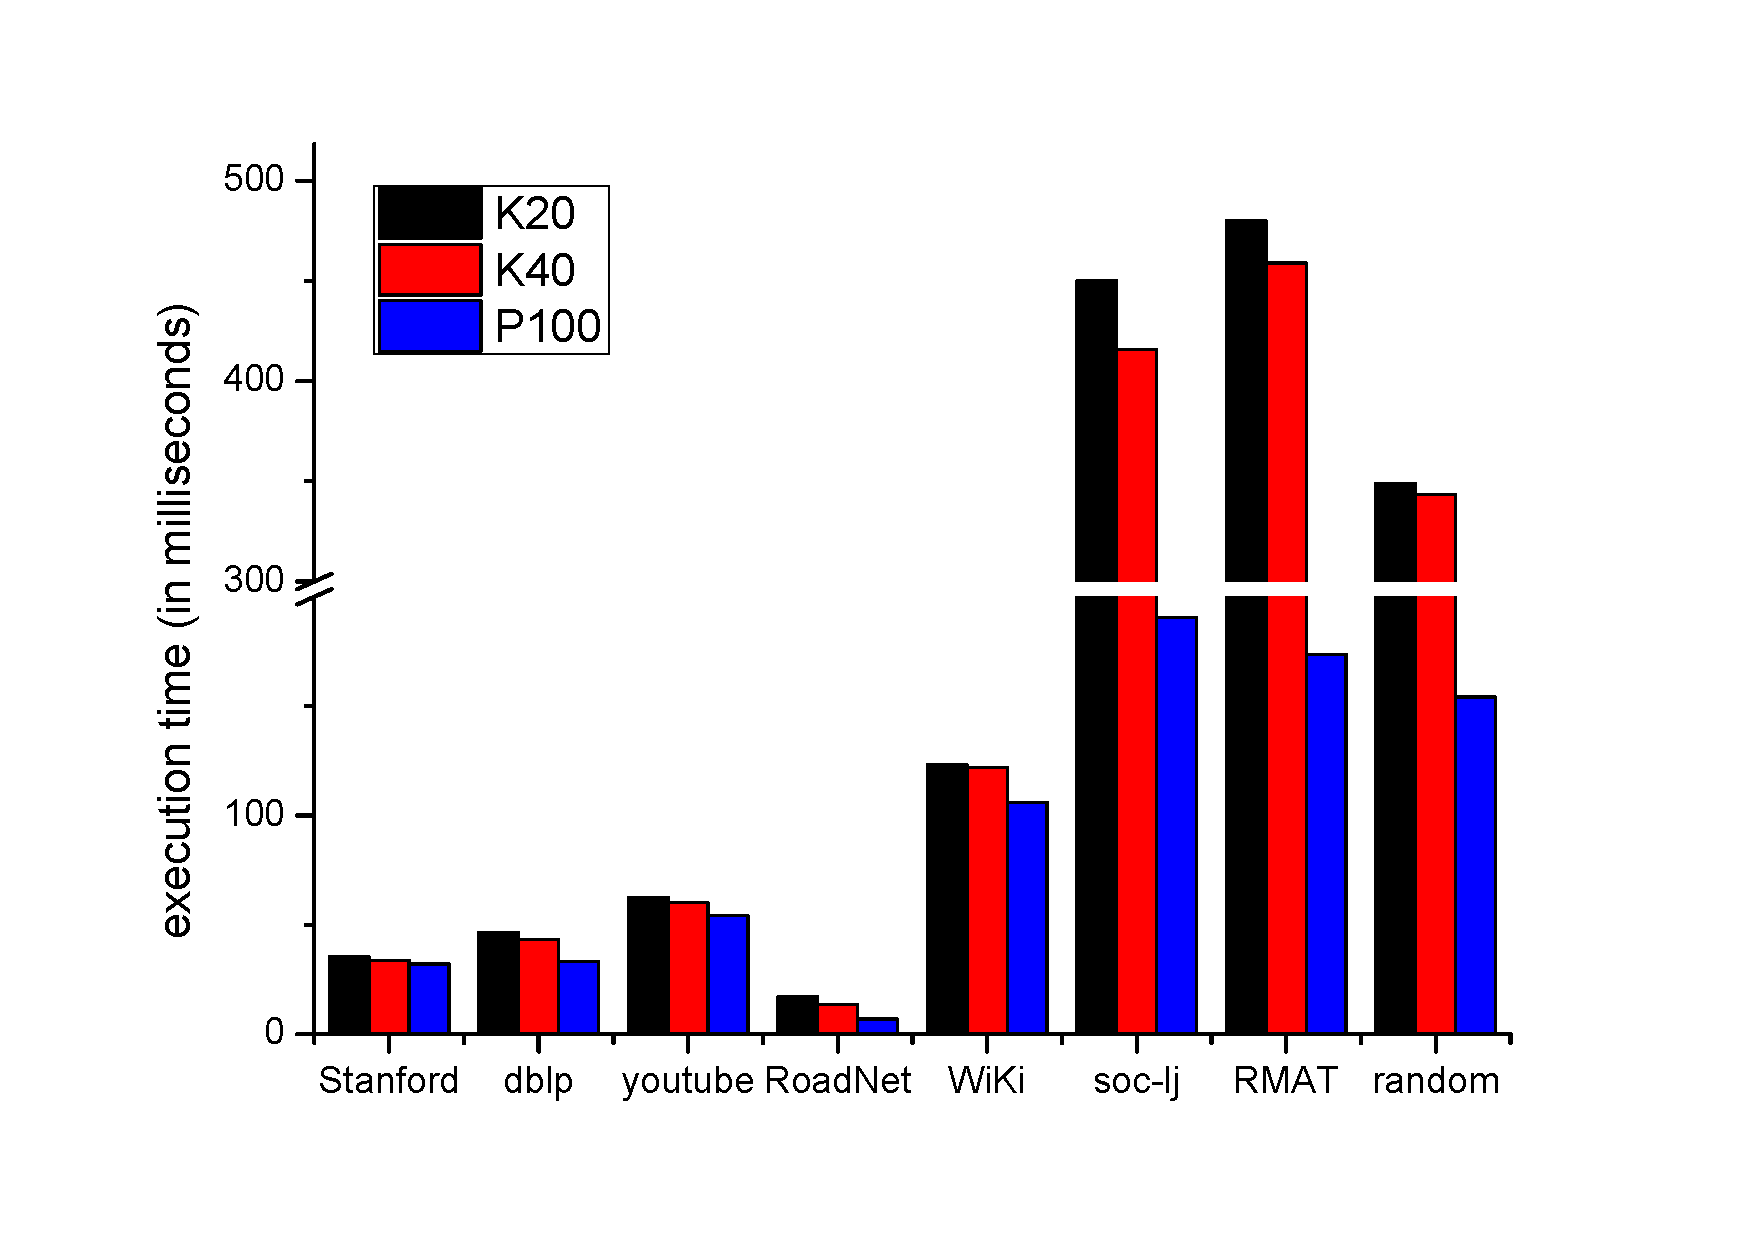
\includegraphics[scale=0.25]{figure/scale.pdf}
	\caption{The performance of Feluca on different GPU devices}
	\label{fig:scale}%
\end{figure}
\section{Related Work}
\label{relatework}
Most previous research conducted on graph coloring 
focus on the algorithm design and how to find the chromatic 
number \cite{topc,cor}. FastColor is an iteration-based graph 
coloring algorithm for very large graphs \cite{ijcai-17}. FastColor 
sets the lower bound by finding the clique of the working graph $G_k$, which is reduced from the given graph $G$ and becomes smaller during the 
execution of the algorithm. FastColor sets the upper bound by coloring the $G_m$, which 
collects all the vertices and edges that are removed from the given graph 
$G$. By iteratively coloring the $G_k$ and $G_m$, FastColor can obtain the 
final color plan once the upper bound meets the lower bound. Experimental 
results show that FastColor can color the graph with ten million vertices 
and one hundred million edges in several minutes. 

Focusing on the dynamic graph coloring problem, the work in \cite{vldbcolor} proposed a 
color-propagation based algorithm which colors the vertices according to 
the propagation order of vertices. The authors use a directed acyclic graph as 
the auxiliary graph of the given graph. The authors color the auxiliary graph 
first by exploring all vertices in 2-hop neighbors of the active 
vertices. In the color-propagation based algorithm, the vertices need to be 
recolored only if the in-neighbors have been changed. Experimental results 
show that the algorithm can color the graph with ten million vertices 
and one hundred million edges in seconds. 

The work in \cite{ppopp-11} evaluated the features of graph coloring on GPU, which provides some insightful
research directions for other researchers. Reference \cite{sc-16} studied the graph coloring problem and applied it to the infrastructure-level 
online analytic design space. cuSPARSE library \cite{nvidiaTR} is a basic linear 
algebra subroutines developed by NVIDIA. cuSPARSE contains a set of graph processing tools, including the graph coloring algorithm, which is the only 
publicly-available coloring library for SIMD architectures to date. 
Reference \cite{Manycore} proposed a parallel coloring 
algorithm on manycore architectures and the authors implemented the algorithm 
on the kokkos library \cite{kokkos}, which can be executed on both Xeon Phi and 
GPU with different compile options. Experimental results shows the proposed 
algorithm can achieve up to 1.5$\times$ speed up over cuSPARSE.
\section{Conclusion and Future Opportunities}
\label{conclusion}

This paper focuses on the graph coloring problem on GPU. 
The recursion computation model can cause the long tail 
problem, which leads to the low efficiency, while the 
sequential spread computation model can cause other problems 
such as low convergence speed. This paper propose a high performance 
graph coloring algorithm on GPU, called Feluca. Feluca 
combines the recursion model and the sequential spread model, which significantly improves 
the graph coloring efficiency. We also propose the optimization techniques in Feluca to avoid the atomic operations, including the craftly-designed method to eliminate the cyclic paths in graphs and a top-down coloring 
scheme. Experimental results show that Feluca can achieve up to 
344.58$\times$ speed up over the state-of-art work and at the same time uses fewer colors on some datasets.

In the future, we plan to focus on other aspects of graph 
coloring, such as coloring the graphs in hybrid systems, coloring the 
graphs on new devices and coloring the dynamic graph on GPU and new devices.

\begin{acks}
This work is partly supported by National Key R\&D Program of China (No. 2017YFC0803700), two grants 
from the National Science Foundation of China (No. 61772218 and No. 61433019) and a grant 
from the Outstanding Youth Foundation of Hubei Province (No. 2016CFA032).
\end{acks}

\bibliographystyle{ACM-Reference-Format}
\bibliography{acmart}

% If your work has an appendix, this is the place to put it.
%\appendix
\end{document}
